\documentclass[12pt, english]{article}
\usepackage{graphicx}
\usepackage[colorlinks=true, linkcolor=blue]{hyperref}
\usepackage[english]{babel}
\selectlanguage{english}
\usepackage[utf8]{inputenc}
\usepackage[svgnames]{xcolor}
\usepackage{subcaption}
\usepackage{graphics}

\usepackage{listings}
\usepackage{afterpage}
\pagestyle{plain}

\definecolor{dkgreen}{rgb}{0,0.6,0}
\definecolor{gray}{rgb}{0.5,0.5,0.5}
\definecolor{mauve}{rgb}{0.58,0,0.82}

%\lstset{language=R,
%    basicstyle=\small\ttfamily,
%   stringstyle=\color{DarkGreen},
%    otherkeywords={0,1,2,3,4,5,6,7,8,9},
%    morekeywords={TRUE,FALSE},
%    deletekeywords={data,frame,length,as,character},
%    keywordstyle=\color{blue},
%    commentstyle=\color{DarkGreen},
%}

\lstset{frame=tb,
language=R,
aboveskip=3mm,
belowskip=3mm,
showstringspaces=false,
columns=flexible,
numbers=none,
keywordstyle=\color{blue},
numberstyle=\tiny\color{gray},
commentstyle=\color{dkgreen},
stringstyle=\color{mauve},
breaklines=true,
breakatwhitespace=true,
tabsize=3
}

\usepackage{here}


\textheight=21cm
\textwidth=17cm
%\topmargin=-1cm
\oddsidemargin=0cm
\parindent=0mm
\pagestyle{plain}

%%%%%%%%%%%%%%%%%%%%%%%%%%
% La siguiente instrucción pone el curso automáticamente%
%%%%%%%%%%%%%%%%%%%%%%%%%%

\usepackage{color}
\usepackage{ragged2e}

\global\let\date\relax
\newcounter{unomenos}
\setcounter{unomenos}{\number\year}
\addtocounter{unomenos}{-1}
\stepcounter{unomenos}
\gdef\@date{ Course \arabic{unomenos}/ 2019}

\begin{document}

\begin{titlepage}

\begin{center}
\vspace*{-1in}
\begin{figure}[htb]
\begin{center}

\includegraphics[width=8cm]{logo}
\end{center}
\end{figure}

Software Development -  CSE 408\\
\vspace*{0.15in}
COMPUTER SCIENCE AND ENGINEERING DEPARTMENT \\
\vspace*{0.4in}
\begin{large}
ParkIn:A Smart Parking App\\
\end{large}
\vspace*{0.2in}
%\begin{Large}
% \textbf{Max-Diversity} \\
% \end{Large}
% \vspace*{0.3in}
% \begin{large}
% Rafael Martí Cunquero \\
% \end{large}
% \vspace*{0.3in}
\rule{80mm}{0.1mm}\\
\vspace*{0.1in}
\begin{large}
Made by: \\
Md.Rajibul Islam\\
ID:1505001\\
Ahnaf Faisal \\
ID: 1505005 \\
Raihanul Alam Hridoy\\
ID:1505010
\end{large}
%\includegraphics[width=10cm]{LogoFac.jpg}
\end{center}
\end{titlepage}

\newcommand{\CC}{C\nolinebreak\hspace{-.05em}\raisebox{.4ex}{\tiny\bf +}\nolinebreak\hspace{-.10em}\raisebox{.4ex}{\tiny\bf +}}
\def\CC{{C\nolinebreak[4]\hspace{-.05em}\raisebox{.4ex}{\tiny\bf ++}}}

\tableofcontents
\newpage
\section{Abstract}
The number of personal vehicles usage is increasing manifold. People prefer personal vehicles to commute than depend on public transportation. Finding a parking space in most metropolitan areas, especially during the rush hours, is difficult for drivers. Due to this there is a need to provide sufficient parking places coupled with plenty of slots to help the user park his vehicle safely, also to ensure the user does not end up parking on non-parking area and cause discomfort to pedestrian.Due to this there is a need to provide sufficient parking places coupled with plenty of slots to help the user park his vehicle safely, also to ensure the user does not end up parking on non-parking area and cause discomfort to pedestrian. The idea behind our Android Application-“'\textbf{ParkIn}” is to help the user analyse area’s where parking is available and number of slots free in that area.Additionally, the user can pre-book a slot in the area he desires for some consecutive days (along with the daily service) if it is available. This will help reduce the load on the administrator as his physical work reduces drastically and user can search the parking slot through Android Application.User can pay after completion of parking service he received. “\textbf{ParkIn}” Application relieves the user
from the hassle of manually searching and waiting for empty slots to park the vehicle.

\section{Introduction}
Android is an operating system, developed for mobile devices like Smartphone’s and tablet computer, which is based on Linux operating system.With the rapid proliferation of vehicle availability and usage in recent years, finding a vacant vehicle parking space is becoming more and more difficult, resulting in a number of practical conflicts.Parking problems are becoming ubiquitous and ever growing at an alarming rate in every major city. Wide usage of android technology with the recent advances in wireless applications for parking, manifests that digital data dissemination could be the key to solve emerging parking problems.Now-a-days there is a steady increase in the number of people using Android mobile phones.We intoduce a Smart Parking System based on android technology for avoiding the parking problems which provides process of pre-booking the slots through the use of a simple and interactive Android application. This application is expected to provide an efficient and cost-effective solution to the effluent vehicle parking problems.The user needs to have an Android enabled device to reap the benefits of this application. After installing the “\textbf{ParkIn}”
app, user needs to mandatorily register with the application. Booking of the slot at user’s desired location should be done prior to the arrival.
Penalty will be levied on late arrival as well as on over use of the slot after user specified entry and exit time. The places where security surveillance (CCTVs) is made available will be used by the administrator to keep a track of the vacant or occupied slots.Else, physical presence of the administrator at the slot site will be required. During reservation process the client needs to provide with details that includes booking person’s mobile no., vehicle number, expected entry and exit time.

\section{Architectural Design} %Eta o incomplete..aro jinispati add korte hobe
“ParkIn” application is based on the client-server architecture. The client is provided with an interactive Android based user interface for the process of pre-booking of parking slot and renting his garage as a renter. The server side processing will be enabled using PHP and MySQL. The client requests the server for locations where parking is available and the server responds with slots availability.Also,server offers the renter to rent his garage and make a way to earn money.
\begin{figure}[h!]
        \begin{minipage}[b]{1\linewidth}
        \centering
        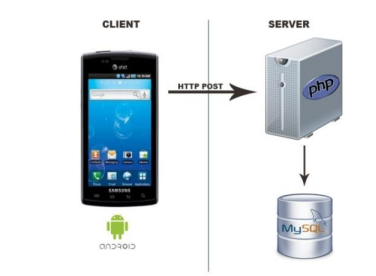
\includegraphics[width=10cm]{architecture.PNG}
        \label{arch}
        \caption{Client Server Architecture of ParkIn App}
        \end{minipage}
\end{figure}

\subsection{Class Diagram}%Class diagram Section
This section contains 2 MVC pattern class diagrams for our design
\newline
Figure \ref{fig:cls_ag1} shows a boundary class \textbf{GarageUI} , a control class \textbf{Garage Addition} and three entity classes: {\textbf{Owner} , \textbf{Garage} , \textbf{Rajuk}}\\
\begin{figure}[h!]
                \centering
                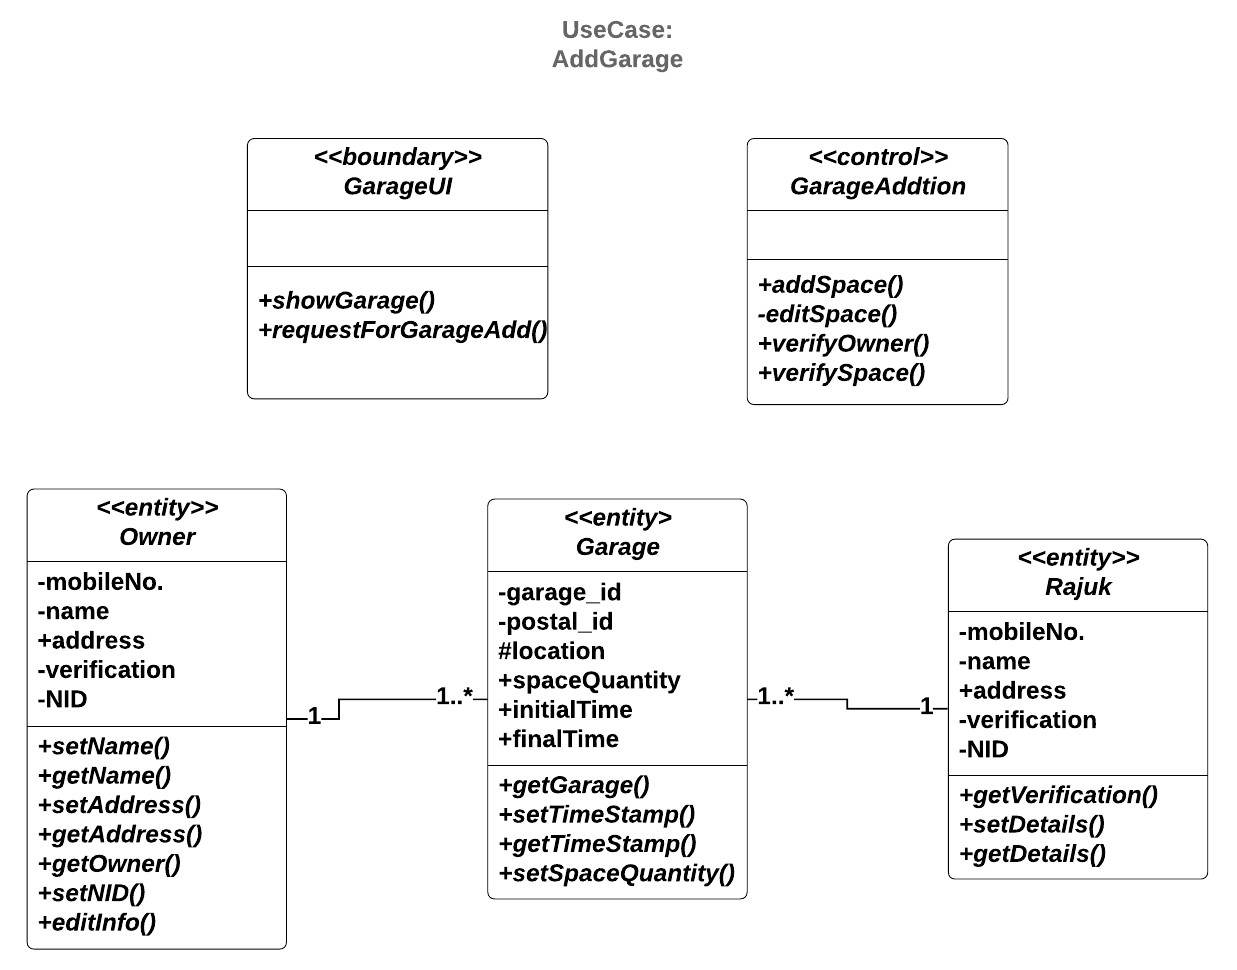
\includegraphics[width=.6\textwidth]{class_ag.png}
                \caption{Class Diagram for Add Garage}
                \label{fig:cls_ag1}
\end{figure}
Figure \ref{fig:cls_ag2} shows a boundary class \textbf{SpaceInqUI} , a control class \textbf{SpaceInq Controller} and two entity classes: { \textbf{Customer} , \textbf{Vehicle}}\\
\begin{figure}[h!]
                \centering
                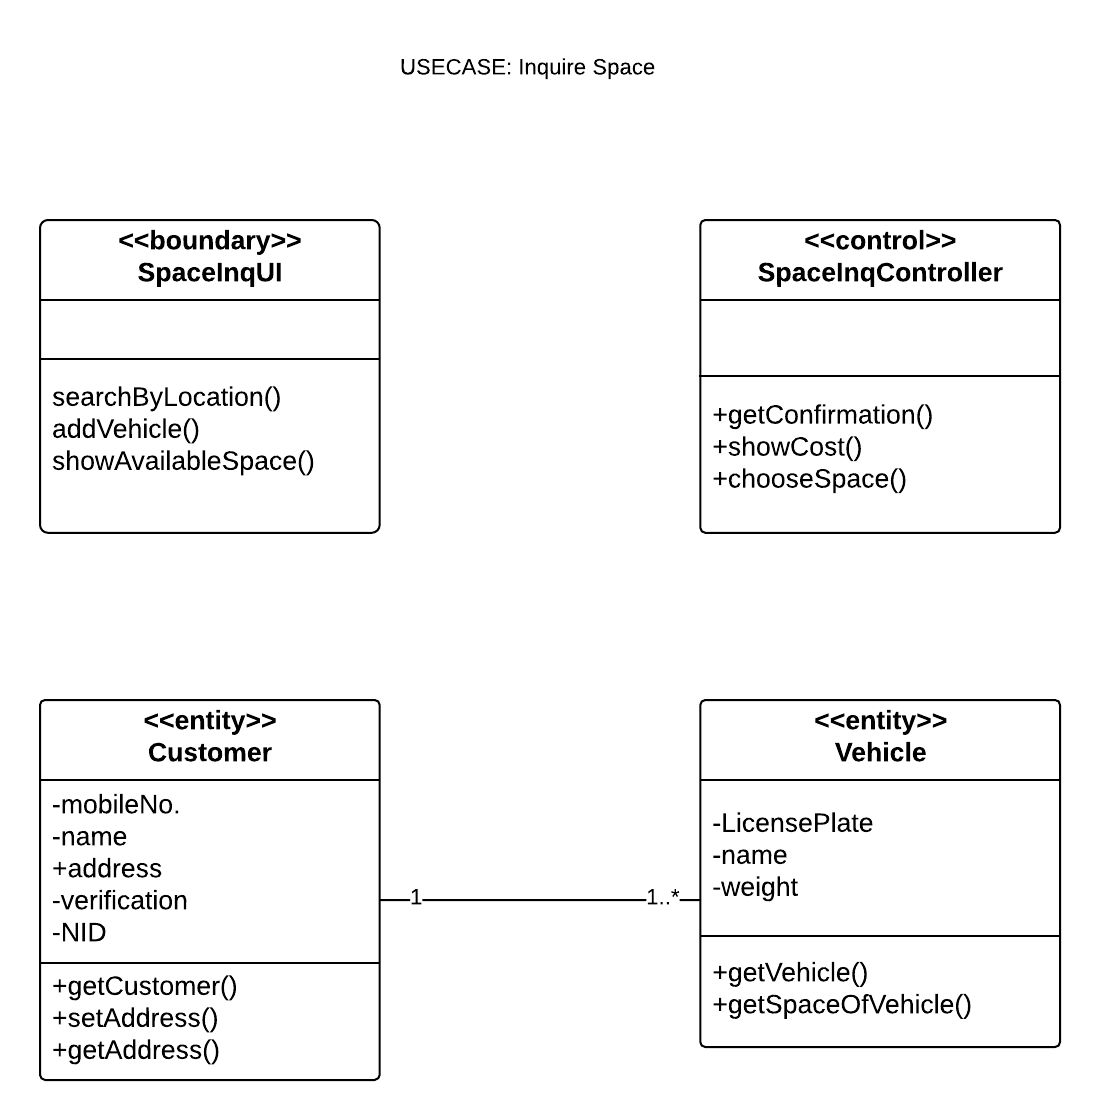
\includegraphics[width=.6\textwidth]{class_inq.png}
                \caption{Class Diagram for Inquire Space}
                \label{fig:cls_ag2}
\end{figure}
\newpage
\subsection{Sequence Diagram}
Figure \ref{fig:seq1} shows the sequence diagram for Add garage usecase.Initially a user interface is loaded and renter actor selects garage from the garage list.After selecting the garage,renter gets the details about the garage.Then, renter adds garage via an instance of Add Garage class and Garage constructor creates new instance for the newly added garage.

\begin{figure}[h!]
                \centering
                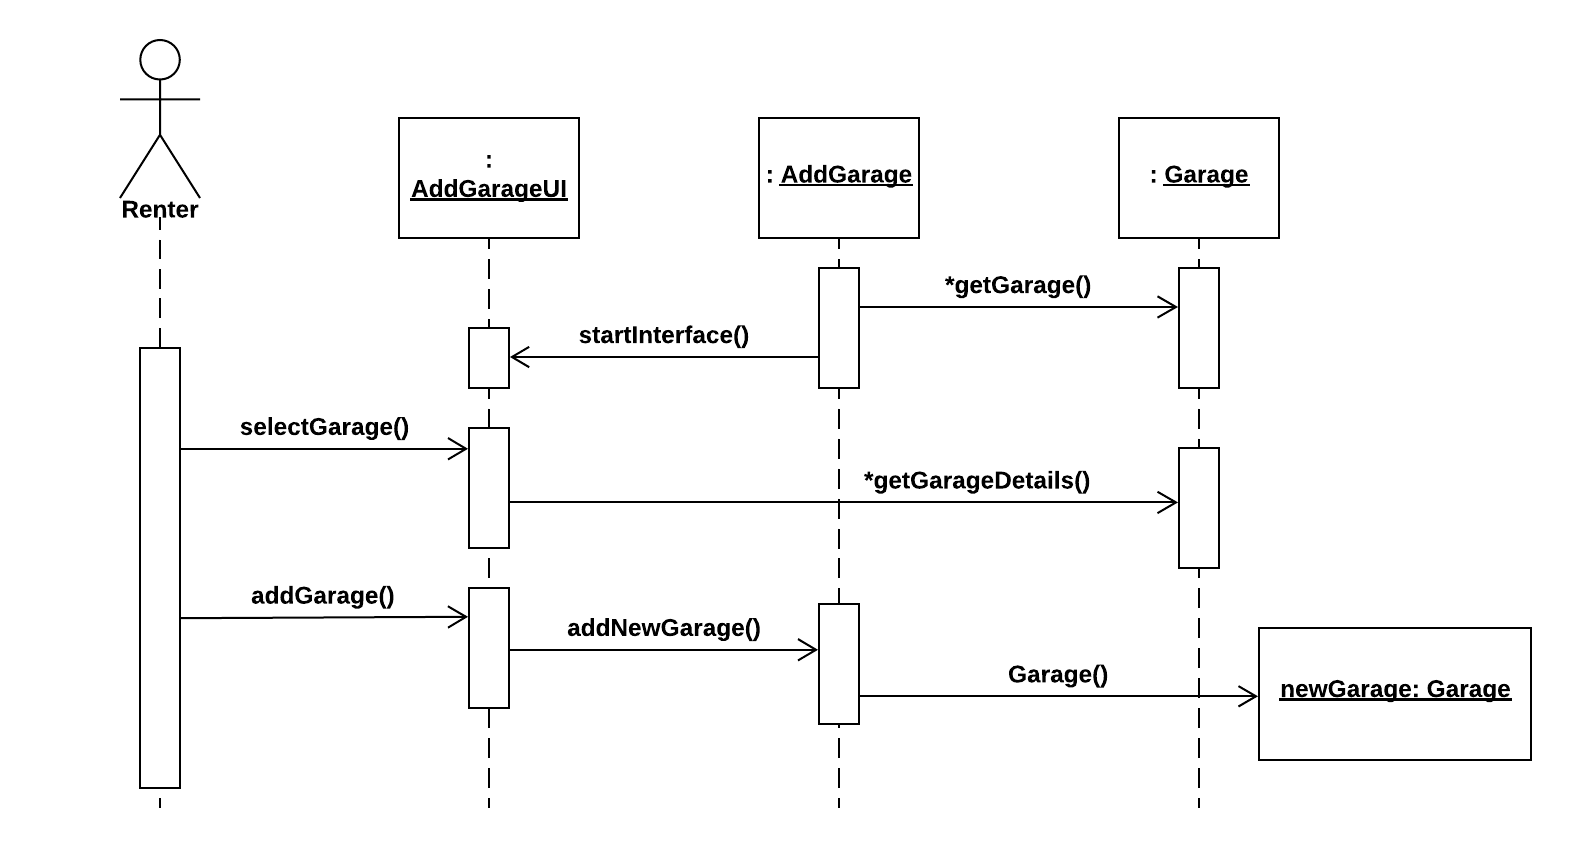
\includegraphics[width=.6\textwidth]{seq1.png}
                \caption{Sequence Diagram for Add Garage}
                \label{fig:seq1}
\end{figure}

Figure \ref{fig:seq2} shows the sequence diagram for Inquire Space Subsystem.At first, customer shows a map with nearest locations with available spaces and choose this space while getSpace method shows the details about the space.Now, customer choose the space to rent if it is available.He/She also adds vehicle via selecting from the vehicle list and confirms the space to rent.
\begin{figure}[h!]
                \centering
                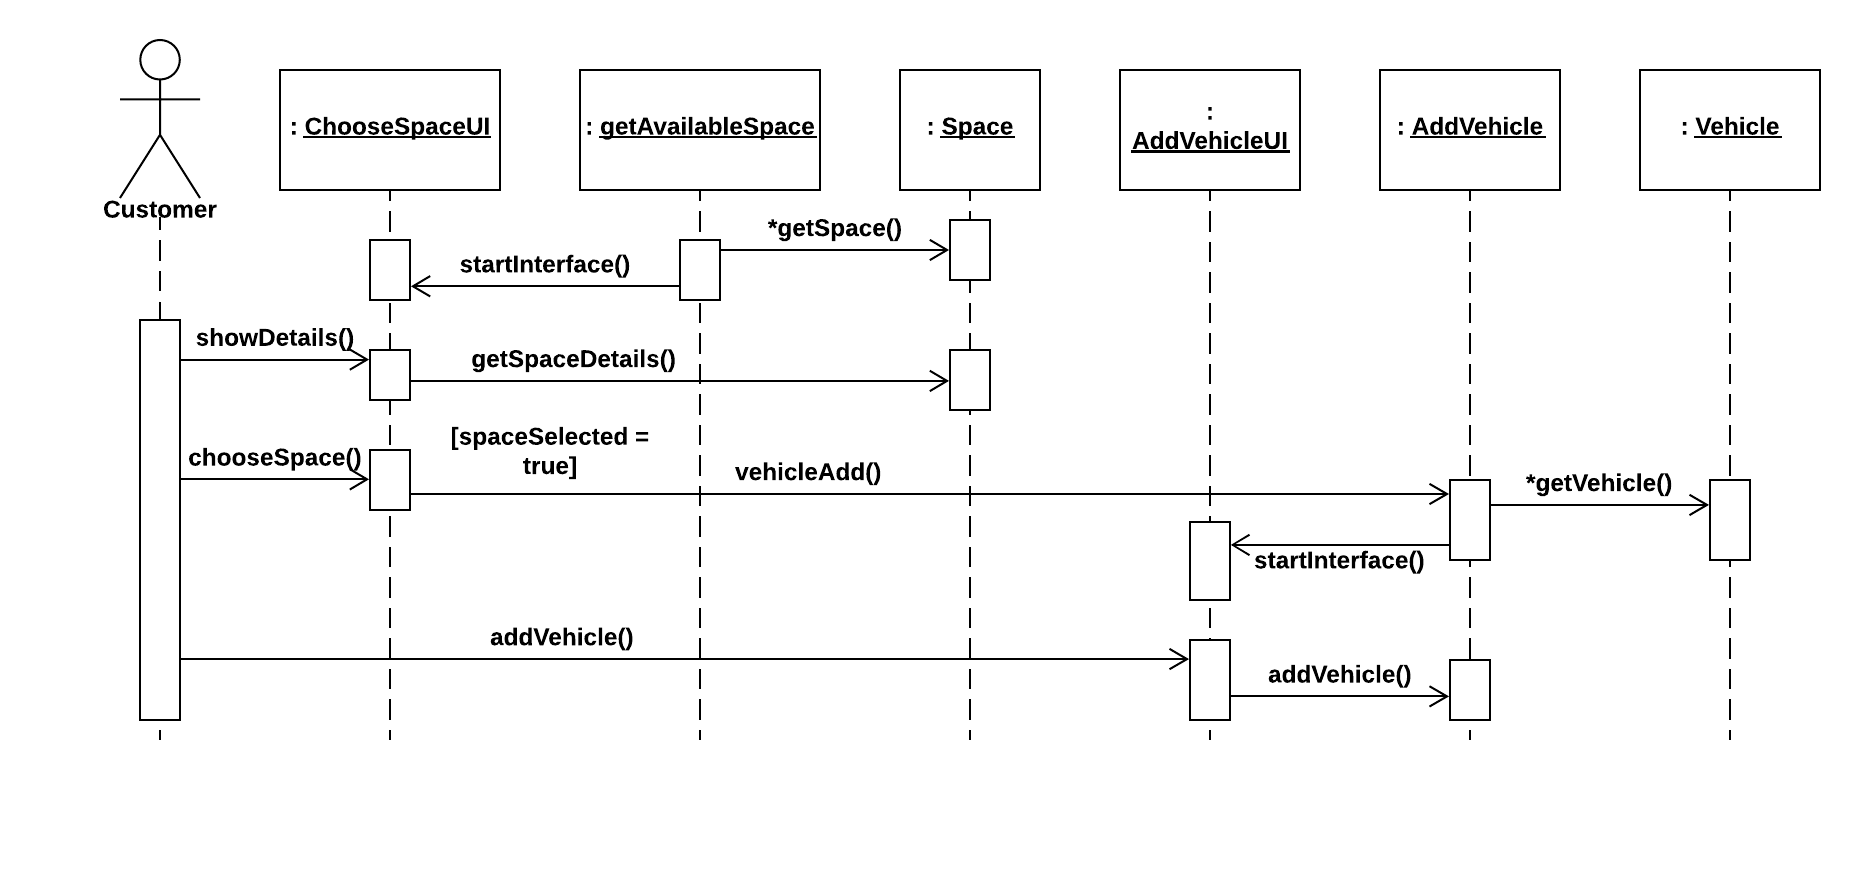
\includegraphics[width=.6\textwidth]{seq2.png}
                \caption{Sequence Diagram for Inquire Space } 
                \label{fig:seq2}
\end{figure}
\newpage

\section{User Guide/Implementation}
\subsection{Client Side}
%In Client side each subsection will contain multiple snapshots and some information how to process..More subsection may be added 
\subsubsection{Starting the Application}
The user needs to install the “ParkIn” application on his Android based device. After installation, the icon of the app will feature on the Home Screen of the user’s device. “ParkIn” Home screen will be flashed to the user on opening the application.
\subsubsection{Registration}
Initially, the user has to register his details with the application for the first time. This is a one-time registration. The user has to enter details like mobile no. as username,name, email-id,address,birthdate etc.All this data will be stored on server and confidentiality will be ensured.
User can then book slot and also rent garage slot using same registered account.We use Google's firebase authentatication system to send verification emails and verify.

\begin{figure}[h!]
    \centering
    \begin{subfigure}[t]{0.4\textwidth}
    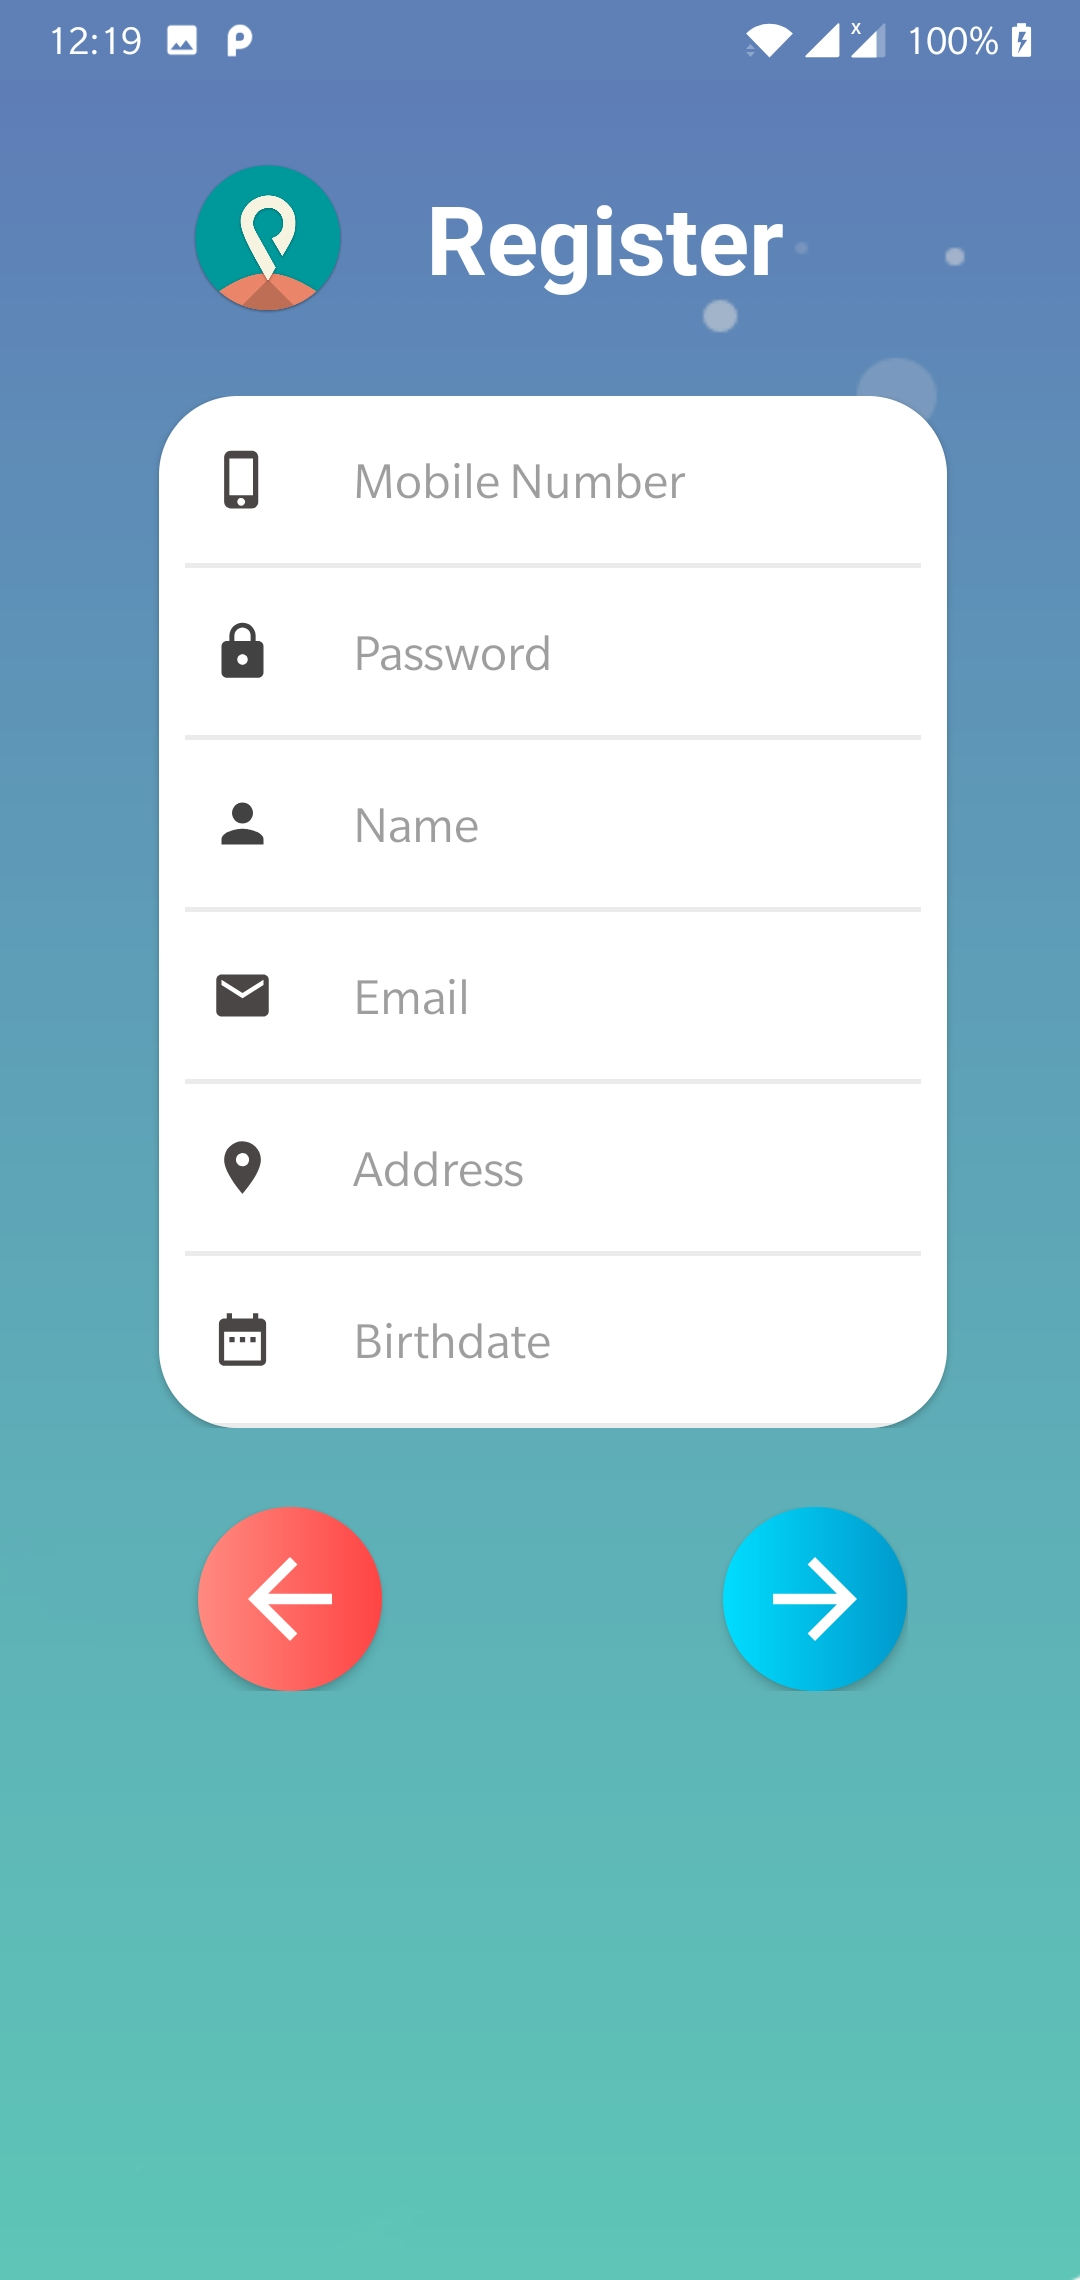
\includegraphics[width=\linewidth]{Account_Creation/CreateAccountActivity.jpg}
     \caption{Account Creation Window}
    \end{subfigure}
    \begin{subfigure}[t]{0.4\textwidth}
    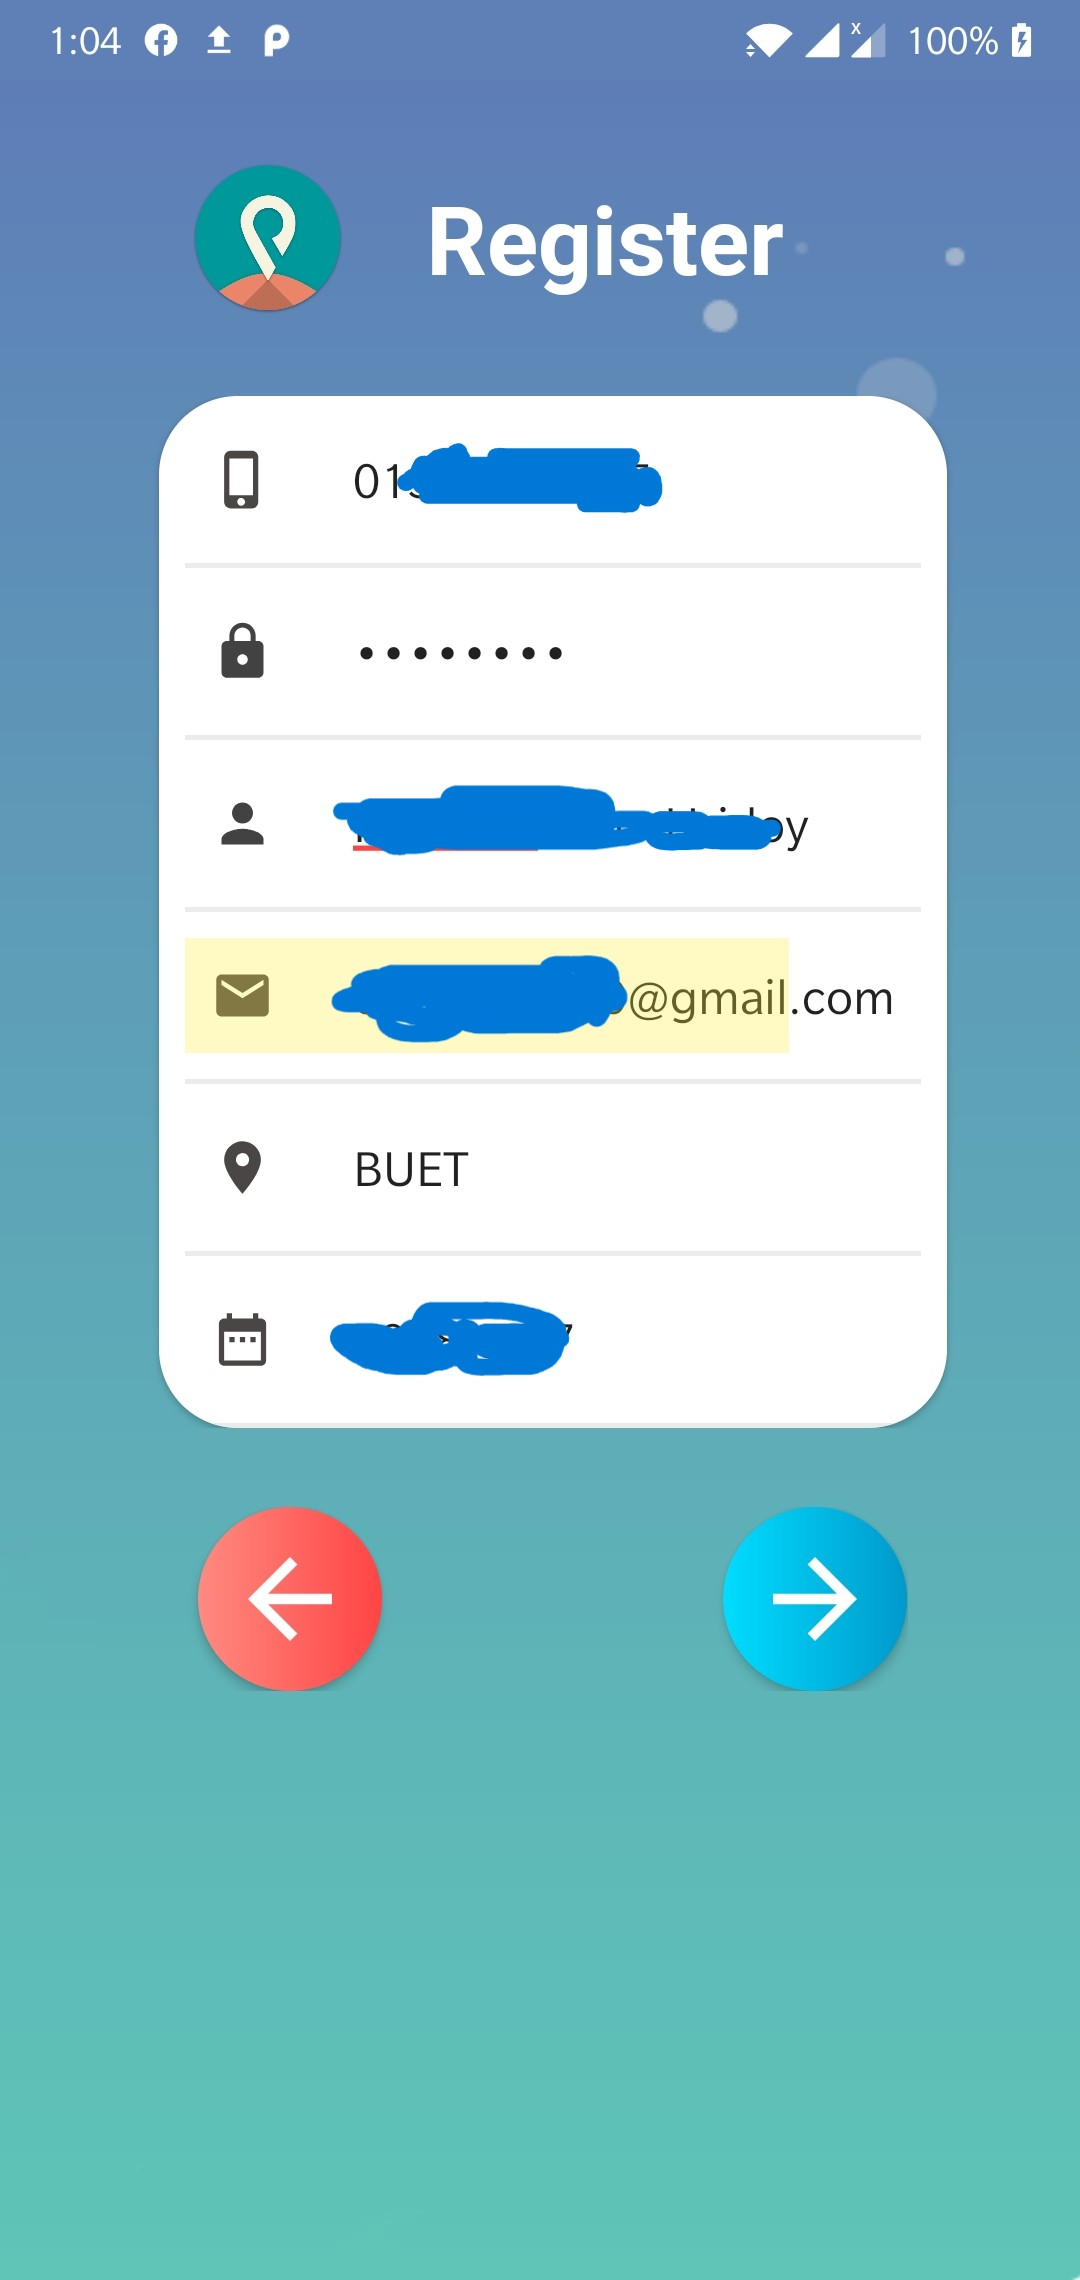
\includegraphics[width=\linewidth]{Account_Creation/CreateAccountActivity_when_details_given.jpg}
    \caption{Account Creation Window with details}
    \end{subfigure}
    \label{fig:arp_os}
\end{figure}


% \begin{figure}[h!]
%         \begin{minipage}[t]{1\linewidth}
%         \centering
%         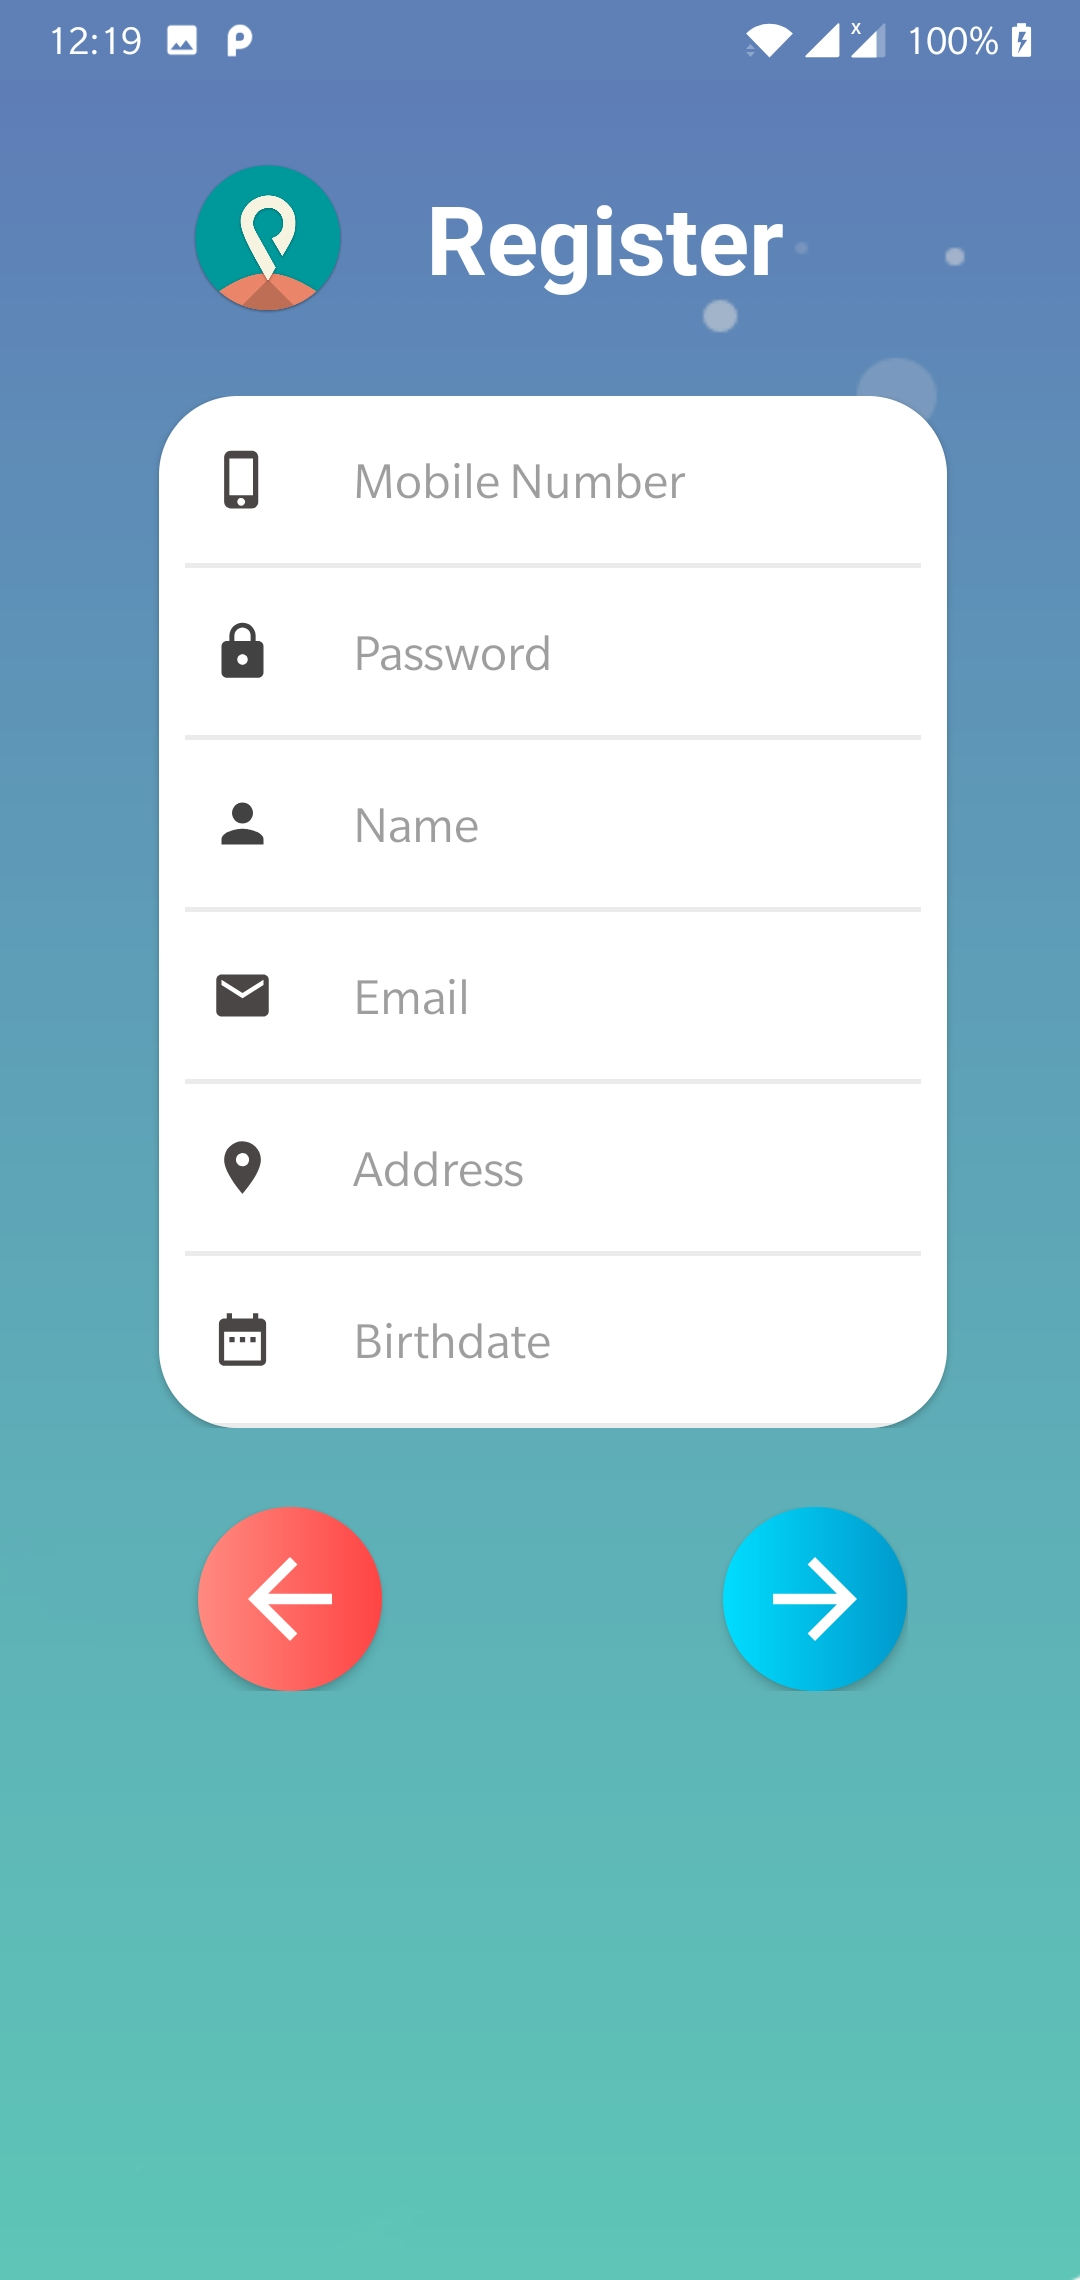
\includegraphics[width=6cm]{Account_Creation/CreateAccountActivity.jpg}
%         \label{arch1}
%         \caption{Account Creation Window}
%         \end{minipage}
% \end{figure}
% \begin{figure}[h!]
%         \begin{minipage}[t]{1\linewidth}
%         \centering
%         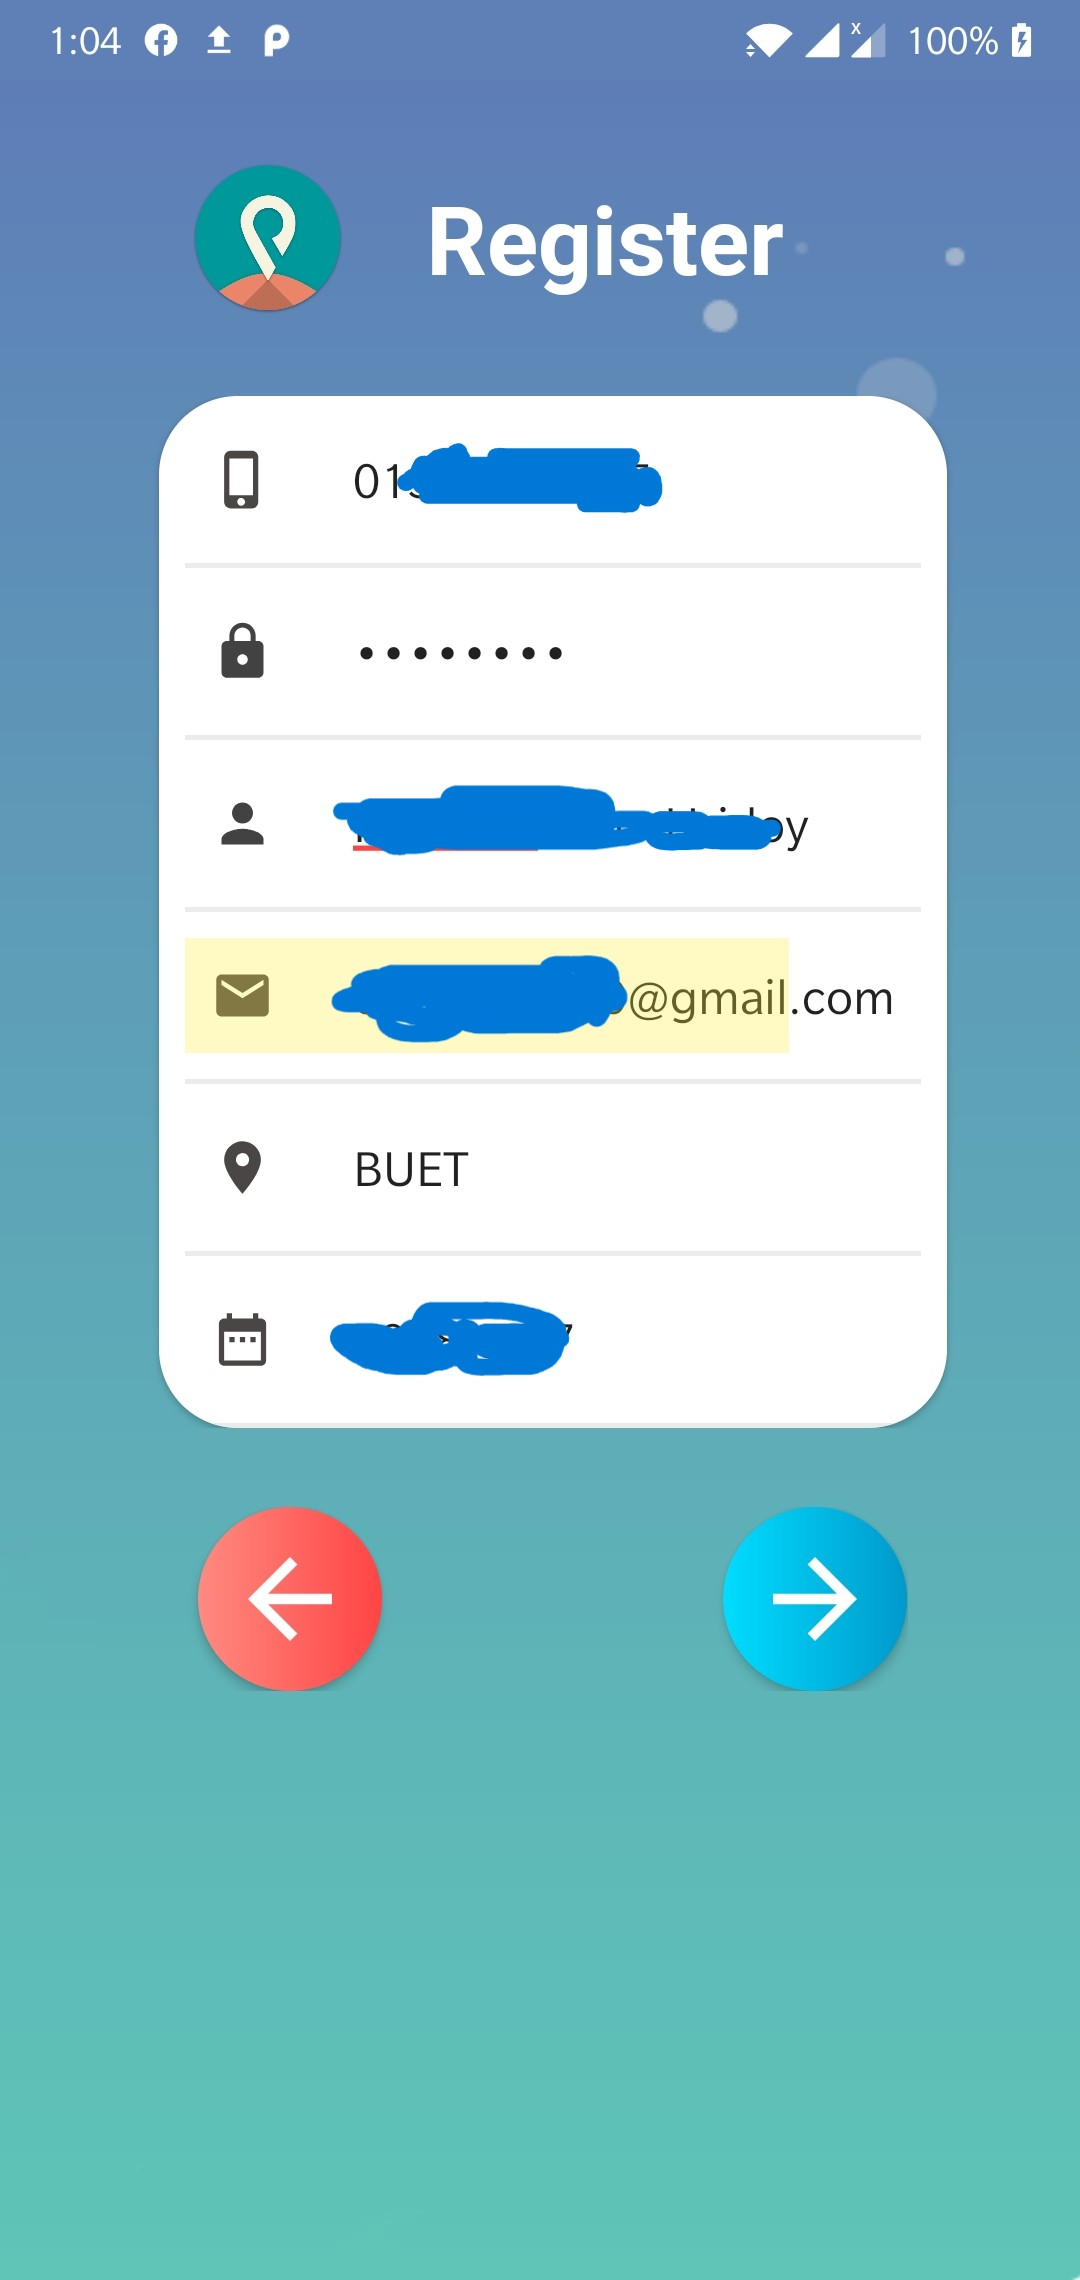
\includegraphics[width=6cm]{Account_Creation/CreateAccountActivity_when_details_given.jpg}
%         \label{arch2}
%         \caption{Account Creation Window with details}
%         \end{minipage}
% \end{figure}


\begin{figure}[h!]
    \centering
    \begin{subfigure}[t]{0.4\textwidth}
    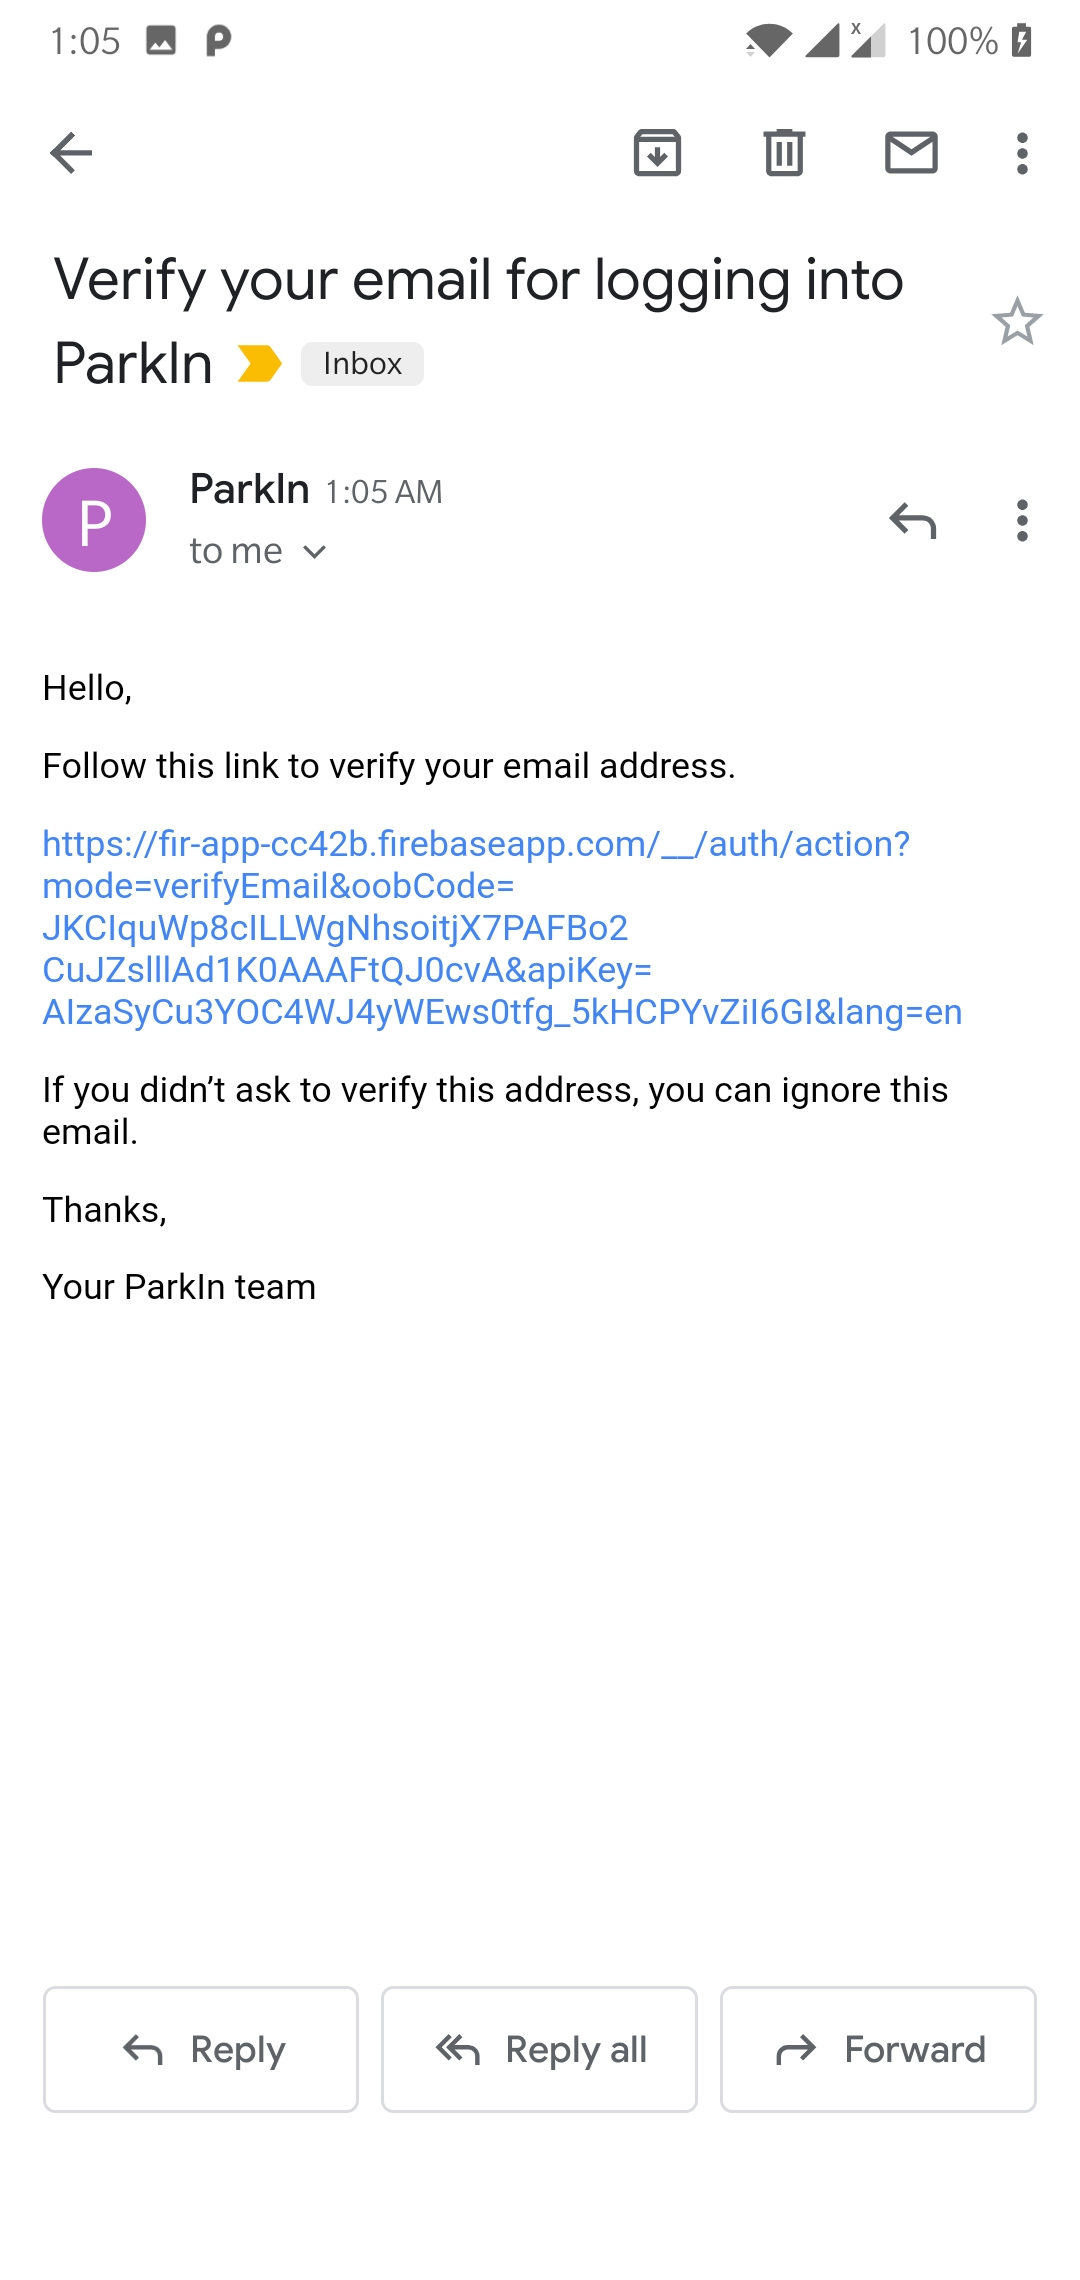
\includegraphics[width=\linewidth]{Account_Creation/Verificationemailsenttoemailaddress.jpg}
     \caption{Verification Email Sent}
    \end{subfigure}
    \begin{subfigure}[t]{0.4\textwidth}
    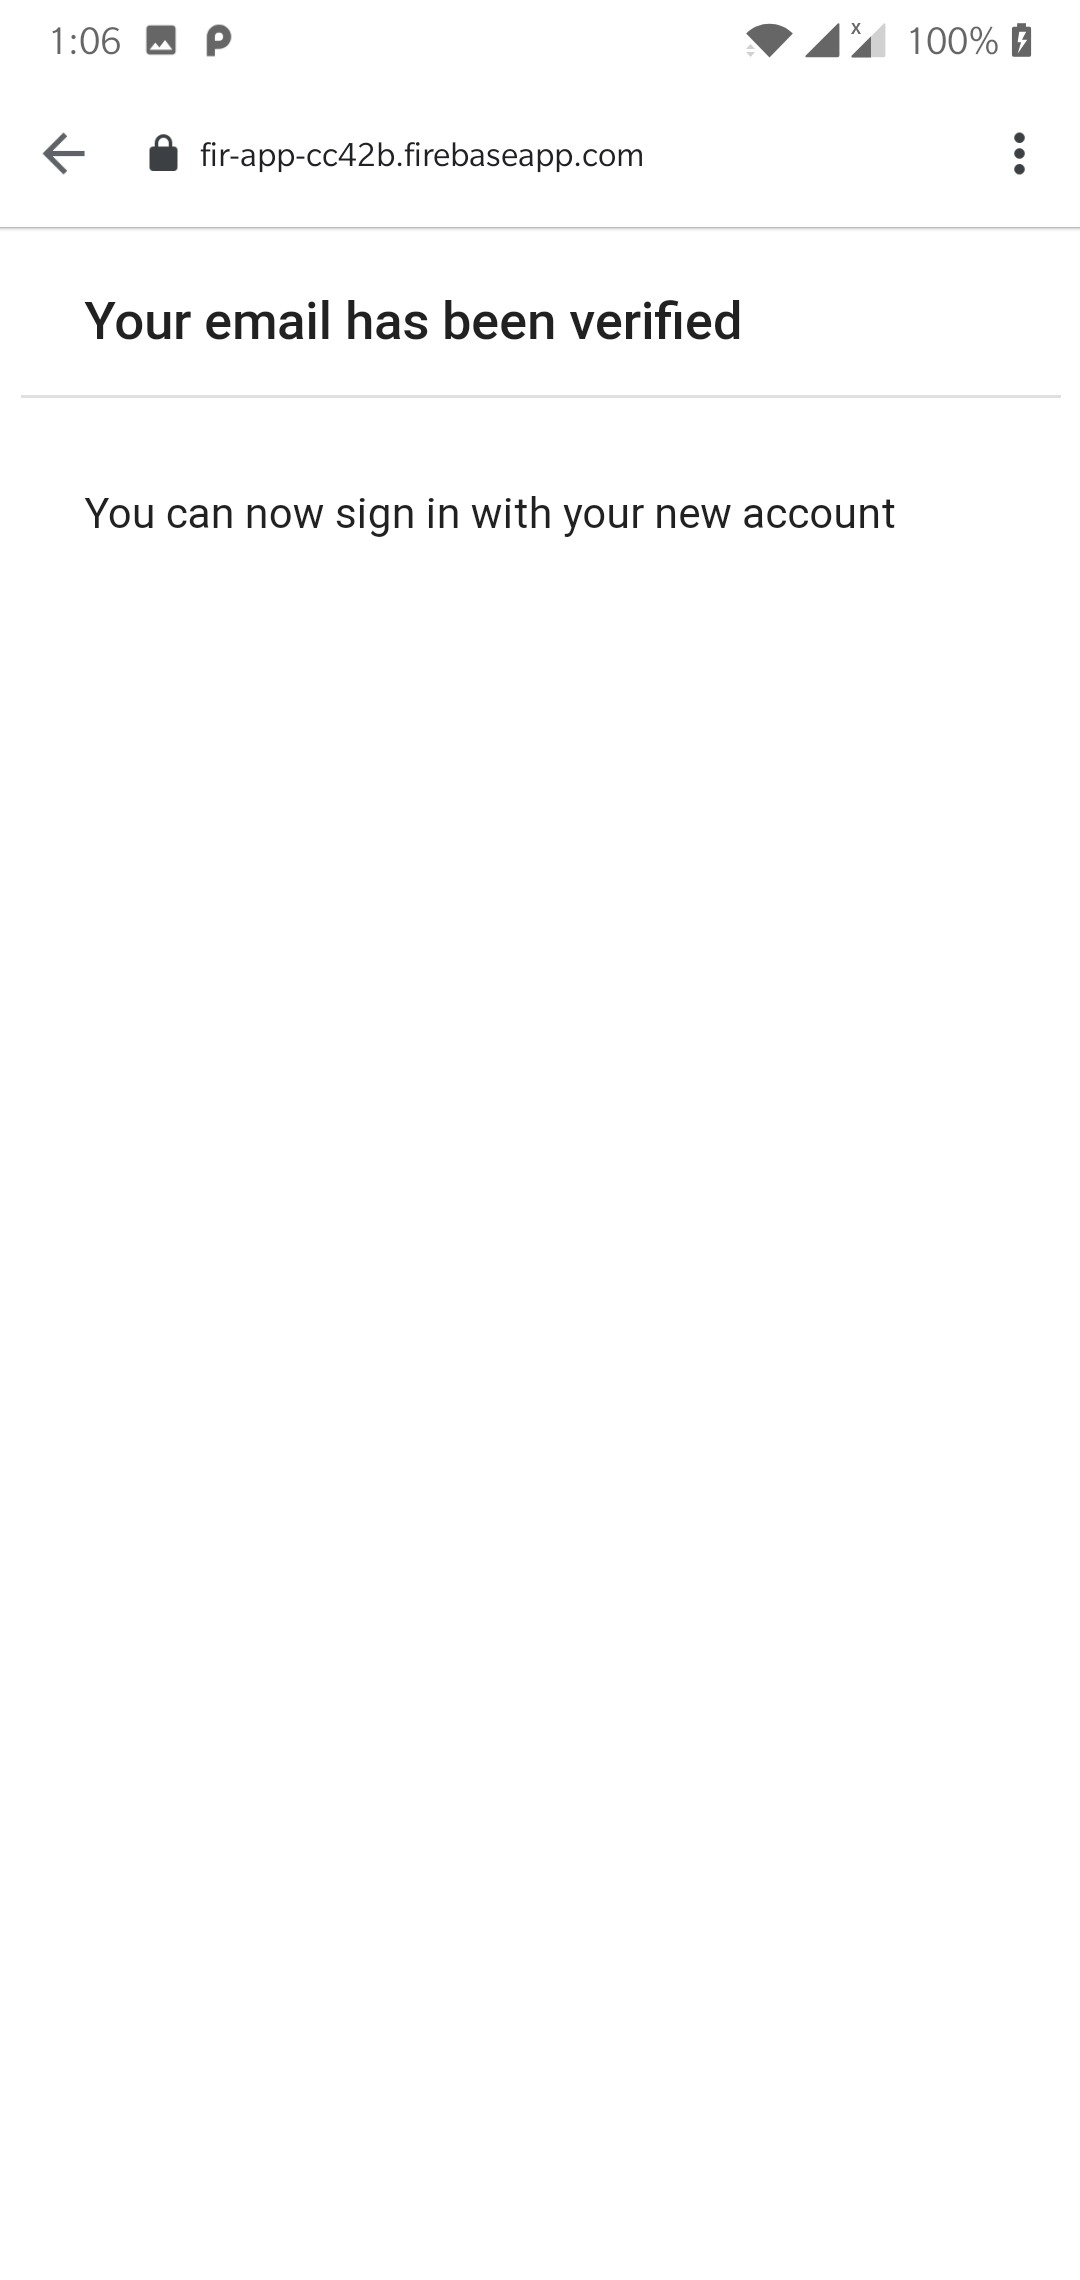
\includegraphics[width=\linewidth]{Account_Creation/email_verified_window.jpg}
        \caption{Email Verified}
    \end{subfigure}
    \label{fig:arp_os}
\end{figure}


% \begin{figure}[h!]
%         \begin{minipage}[b]{1\linewidth}
%         \centering
%         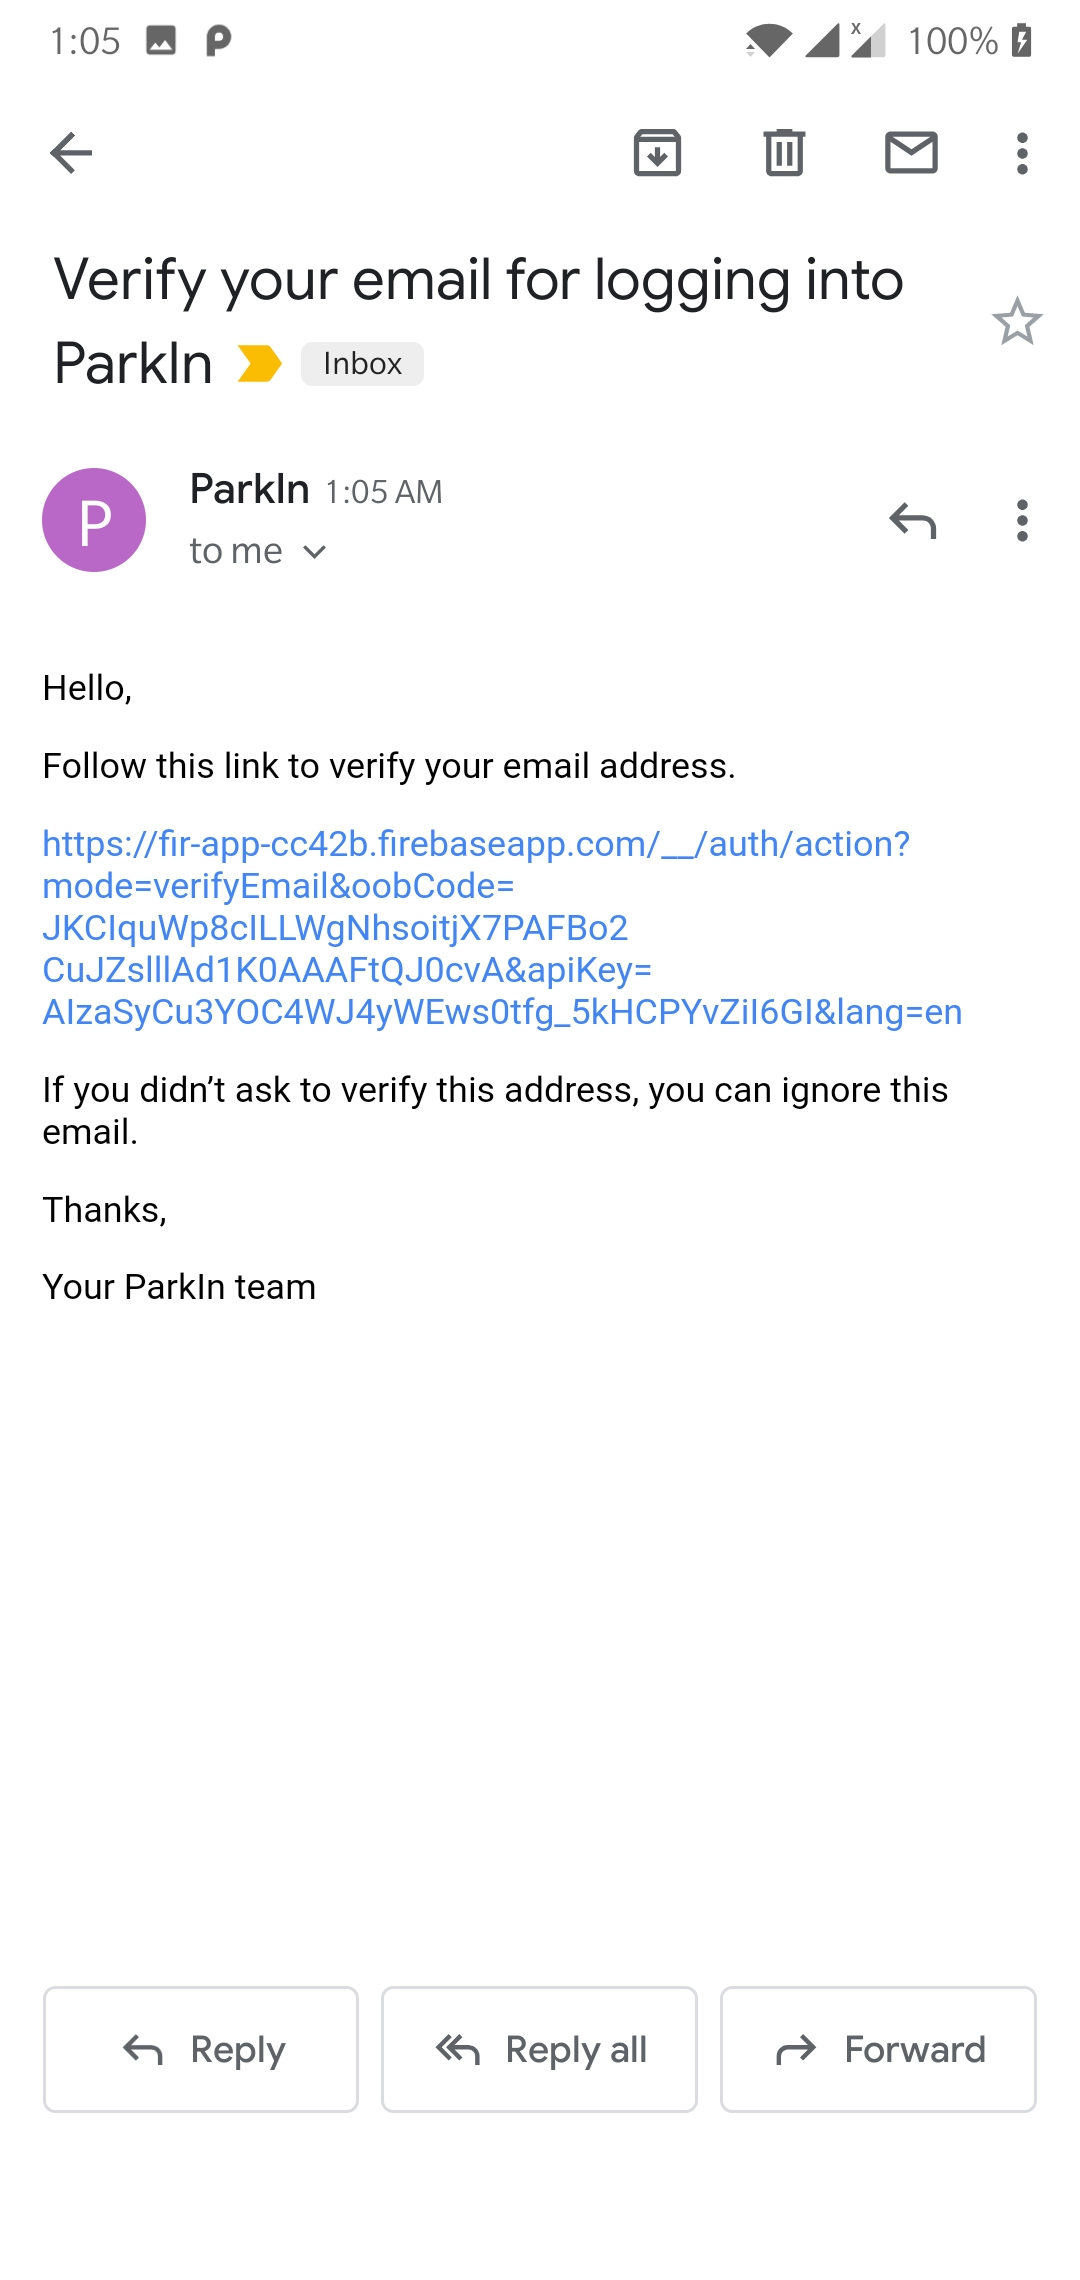
\includegraphics[width=4cm]{Account_Creation/Verificationemailsenttoemailaddress.jpg}
%         \label{arch3}
%         \caption{Email Verified}
%         \end{minipage}
% \end{figure}
% \begin{figure}[h!]
%         \begin{minipage}[b]{1\linewidth}
%         \centering
%         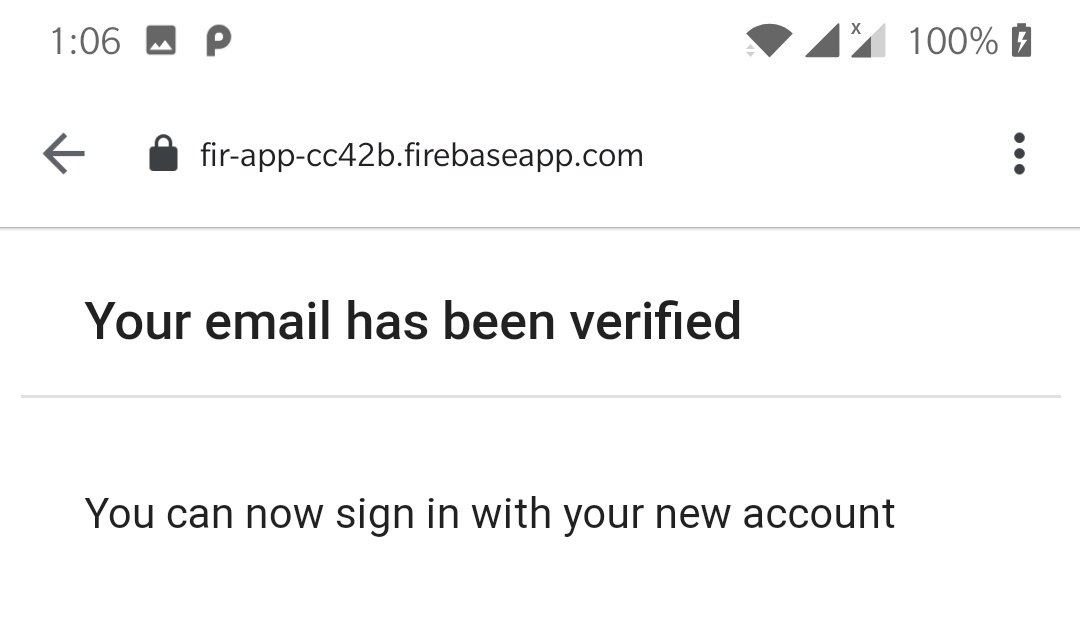
\includegraphics[width=6cm]{Account_Creation/email_verified.jpg}
%         \label{arch4}
%         \caption{Email Verified}
%         \end{minipage}
% \end{figure}


\subsubsection{LogIn}
Once the user registers, he can use his mobile number to login in future. This authenticates the user.After login he can see his profile,history,available garages,vehicles information etc.
\newpage
% \begin{figure}[h!]
%         \begin{minipage}[b]{1\linewidth}
%         \centering
%         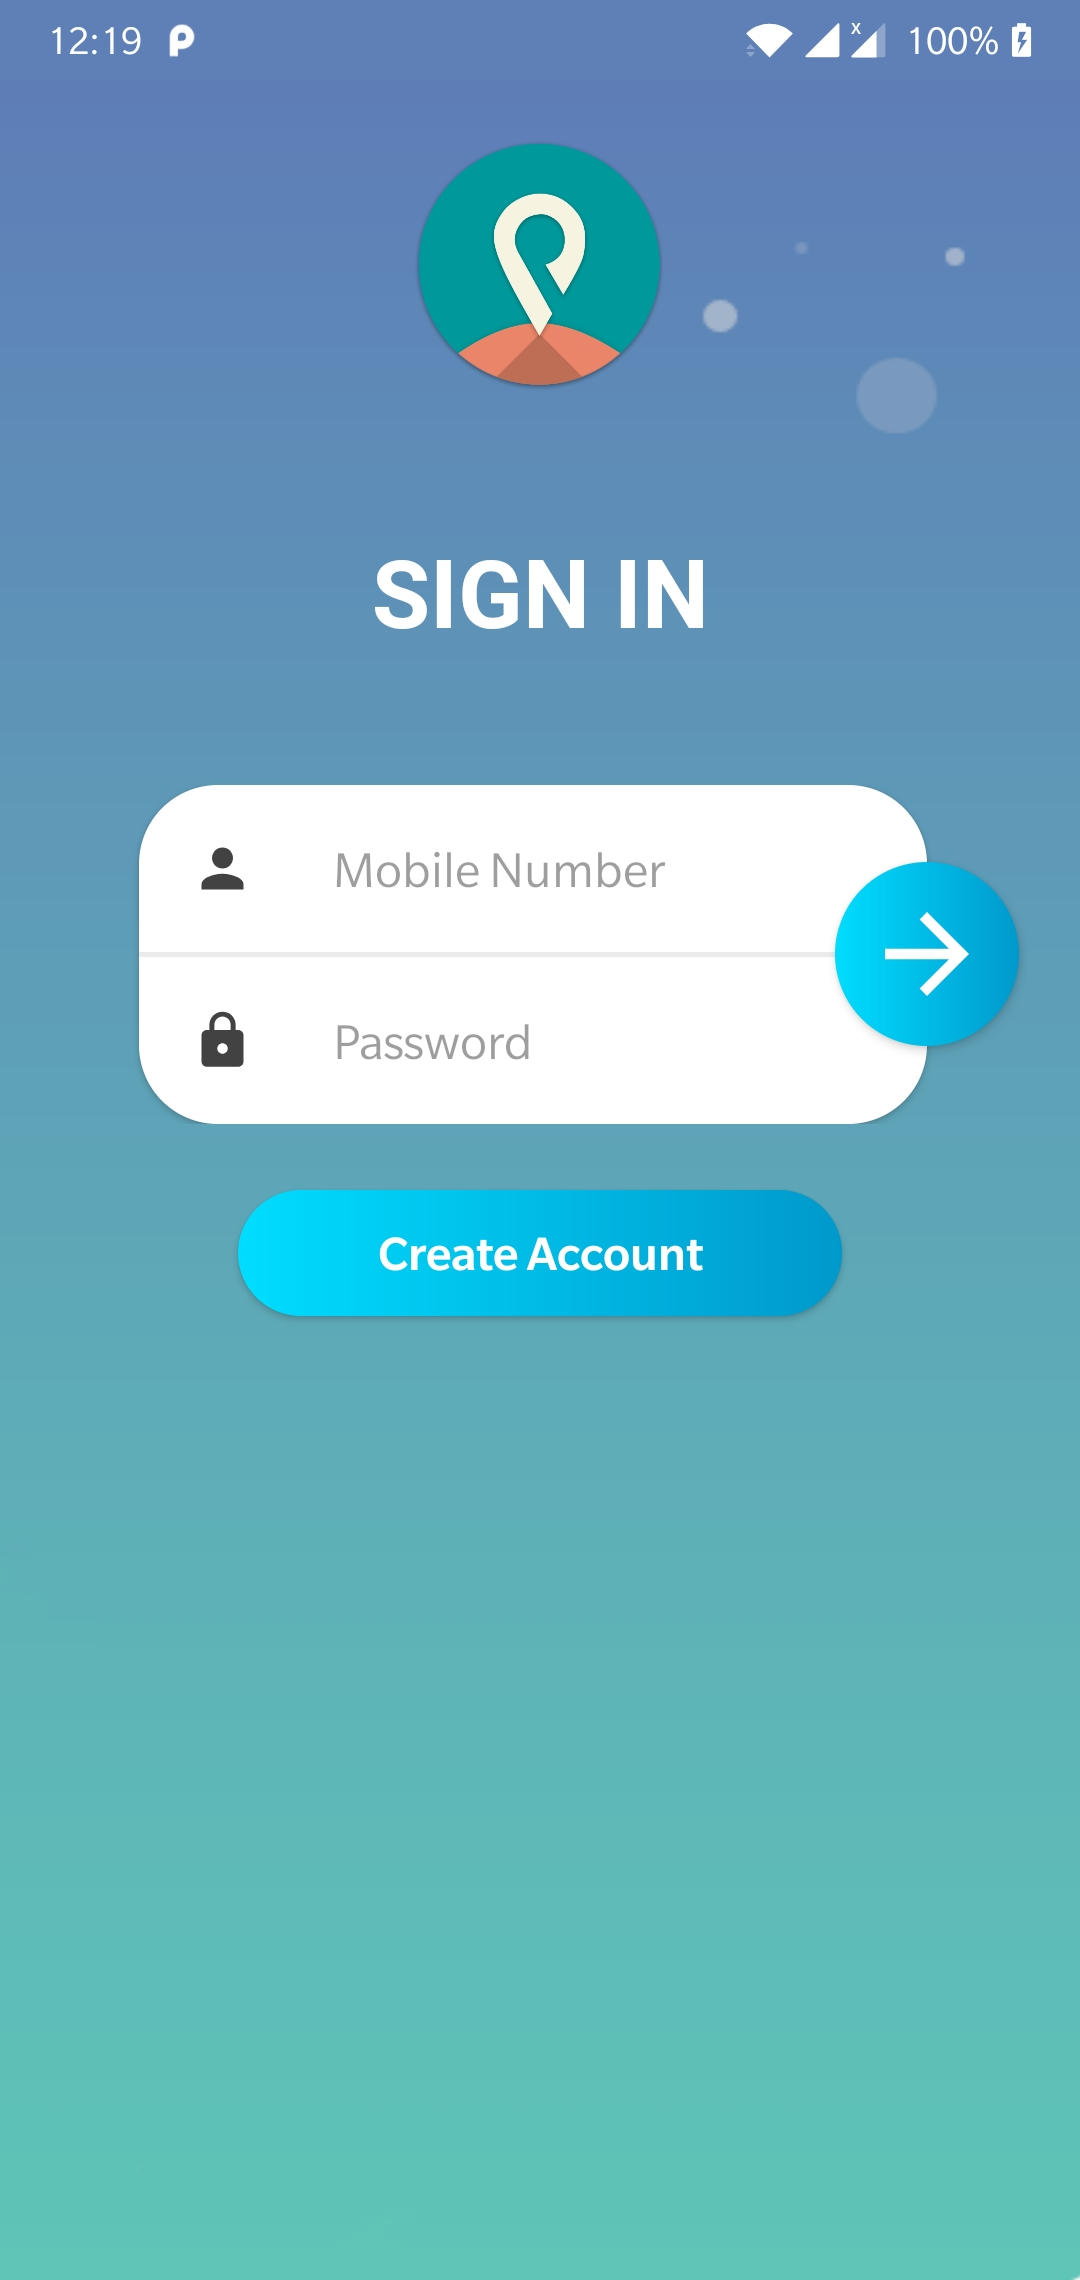
\includegraphics[width=4cm]{LogIn/LoginActivity.jpg}
%         \label{arch5}
%         \caption{Login Window}
%         \end{minipage}
% \end{figure}
\subsection{Home}
From this window user can go to add garage,vehicle or search for parking location,see ongoing status,notifications and logout.
\newpage
% \begin{figure}[h!]
%         \begin{minipage}[b]{1\linewidth}
%         \centering
%         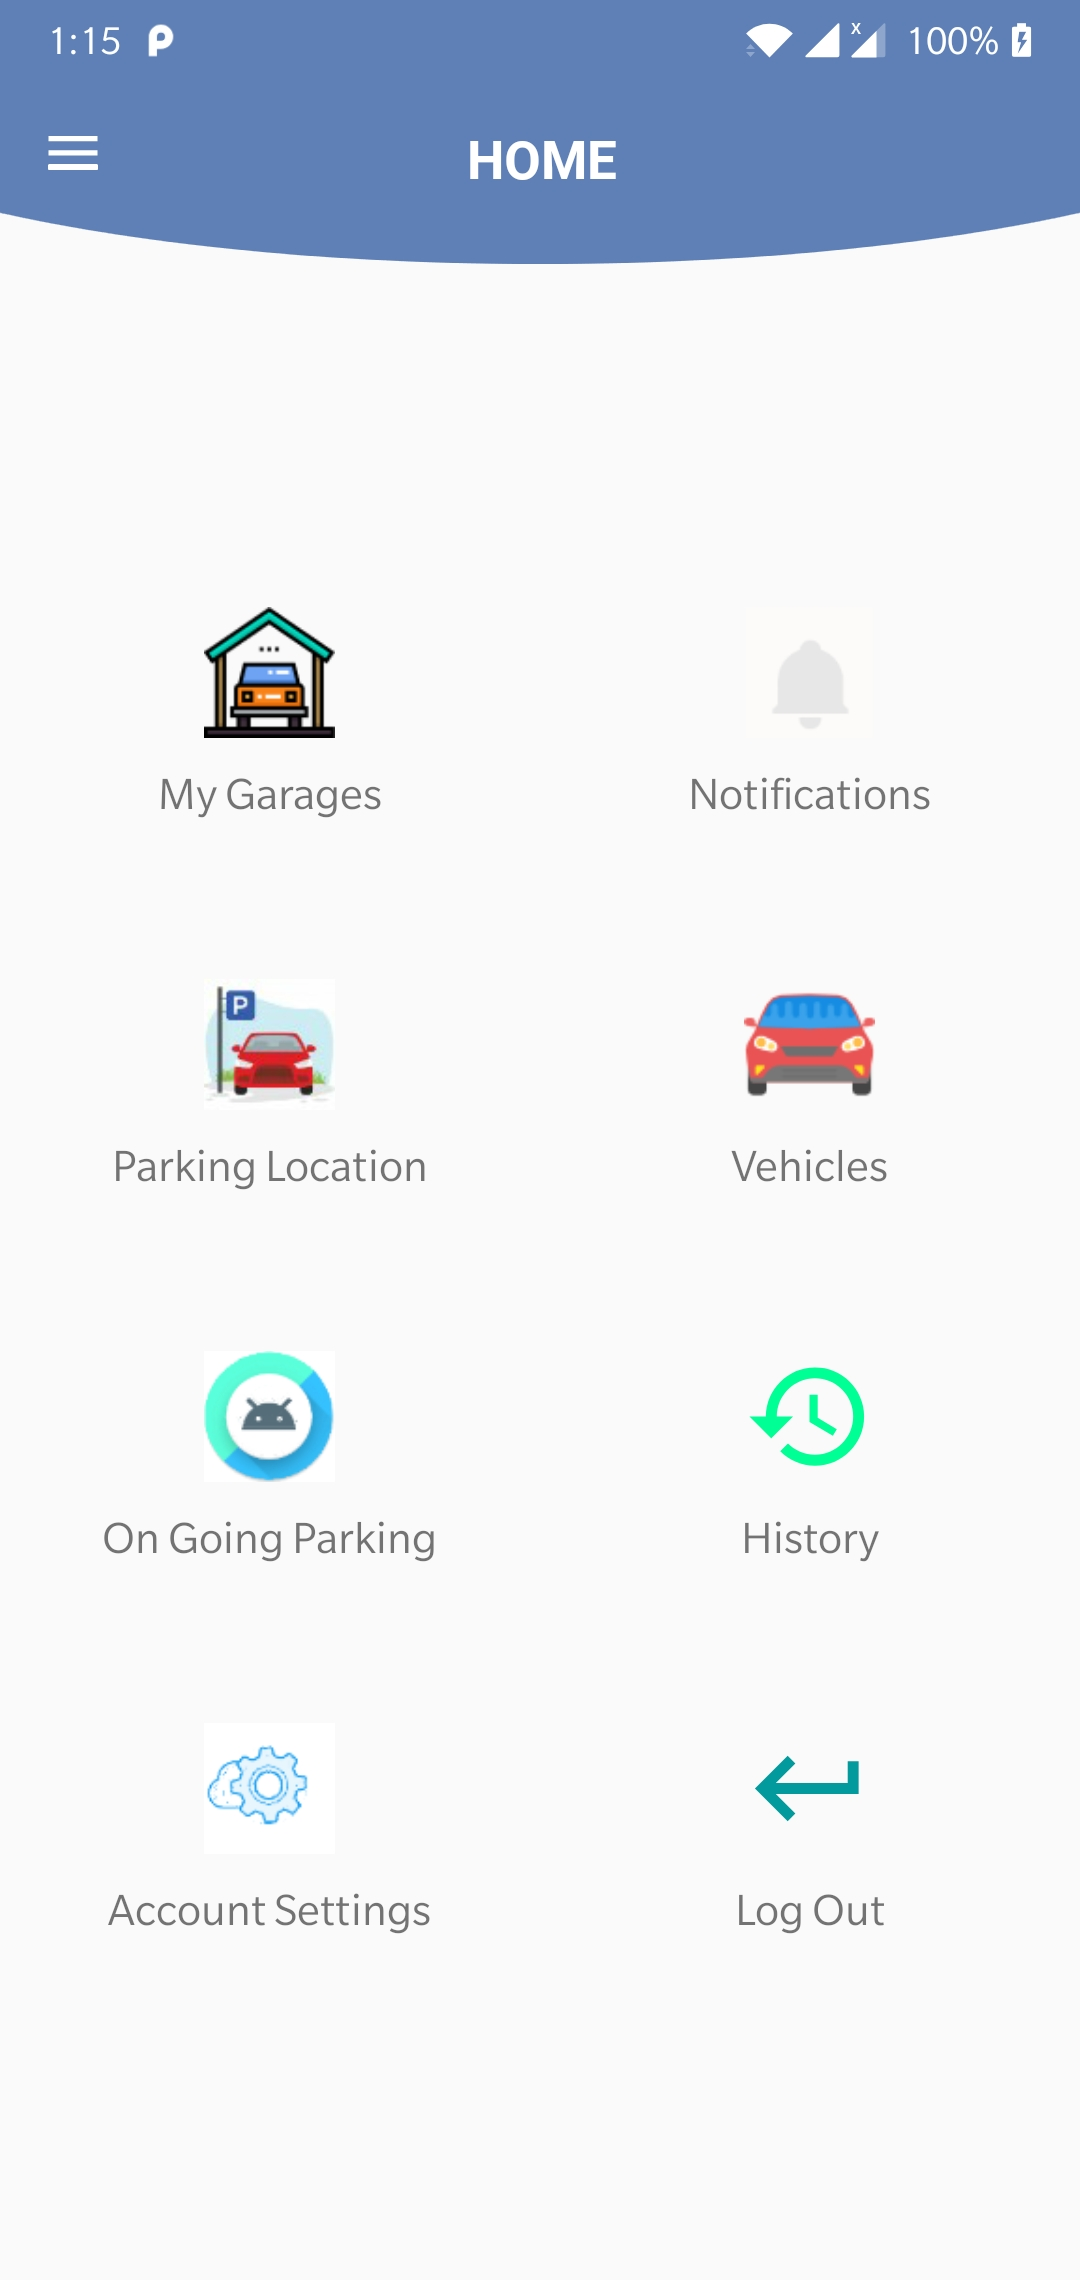
\includegraphics[width=4cm]{HomeActivity.jpg}
%         \label{arch50}
%         \caption{Home window}
%         \end{minipage}
% \end{figure}

\begin{figure}[h!]
    \centering
    \begin{subfigure}[t]{0.4\textwidth}
    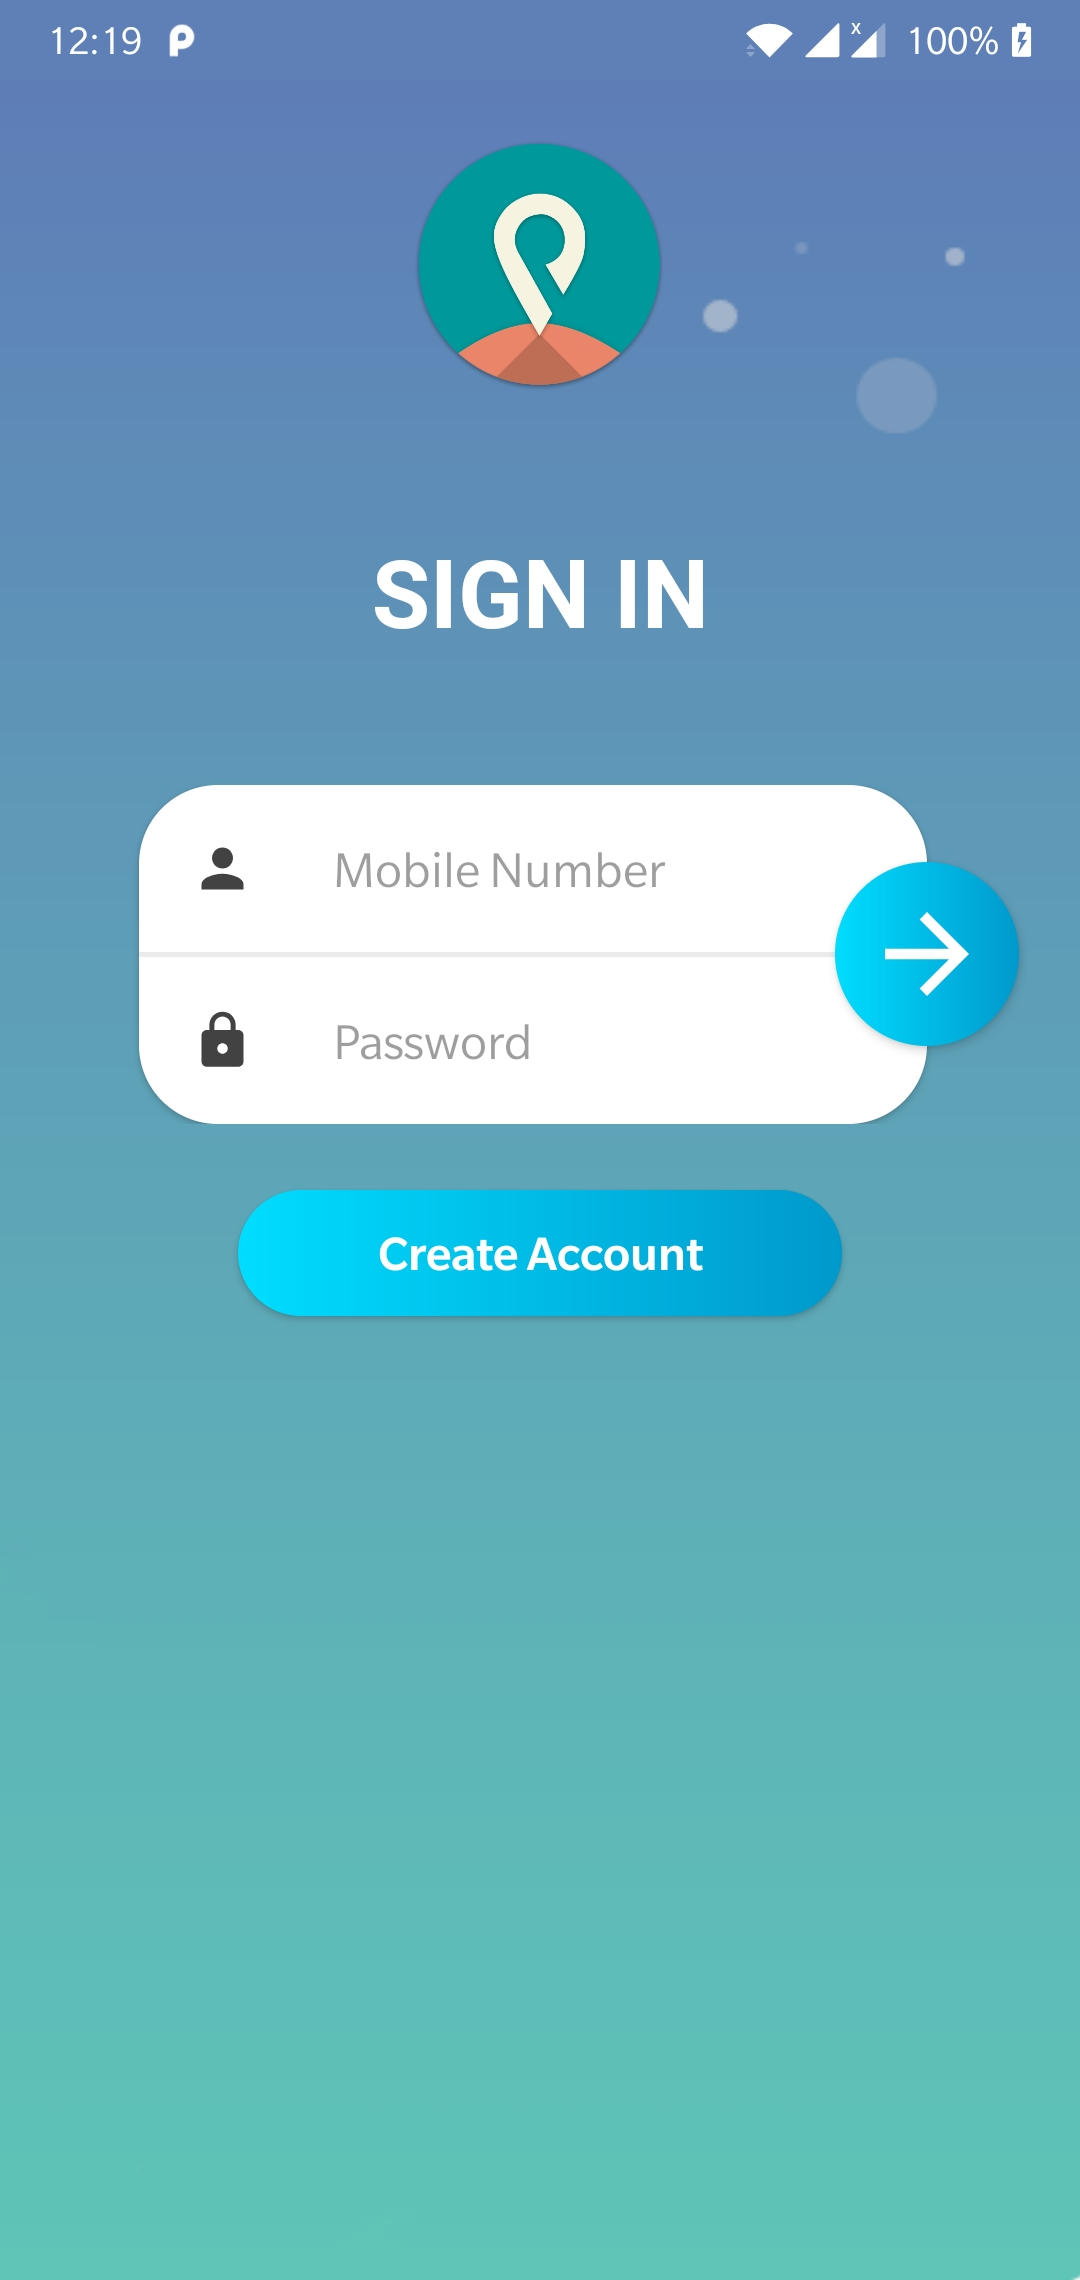
\includegraphics[width=\linewidth]{LogIn/LoginActivity.jpg}
        \label{arch5}
        \caption{Login Window}
    \end{subfigure}
    \begin{subfigure}[t]{0.4\textwidth}
    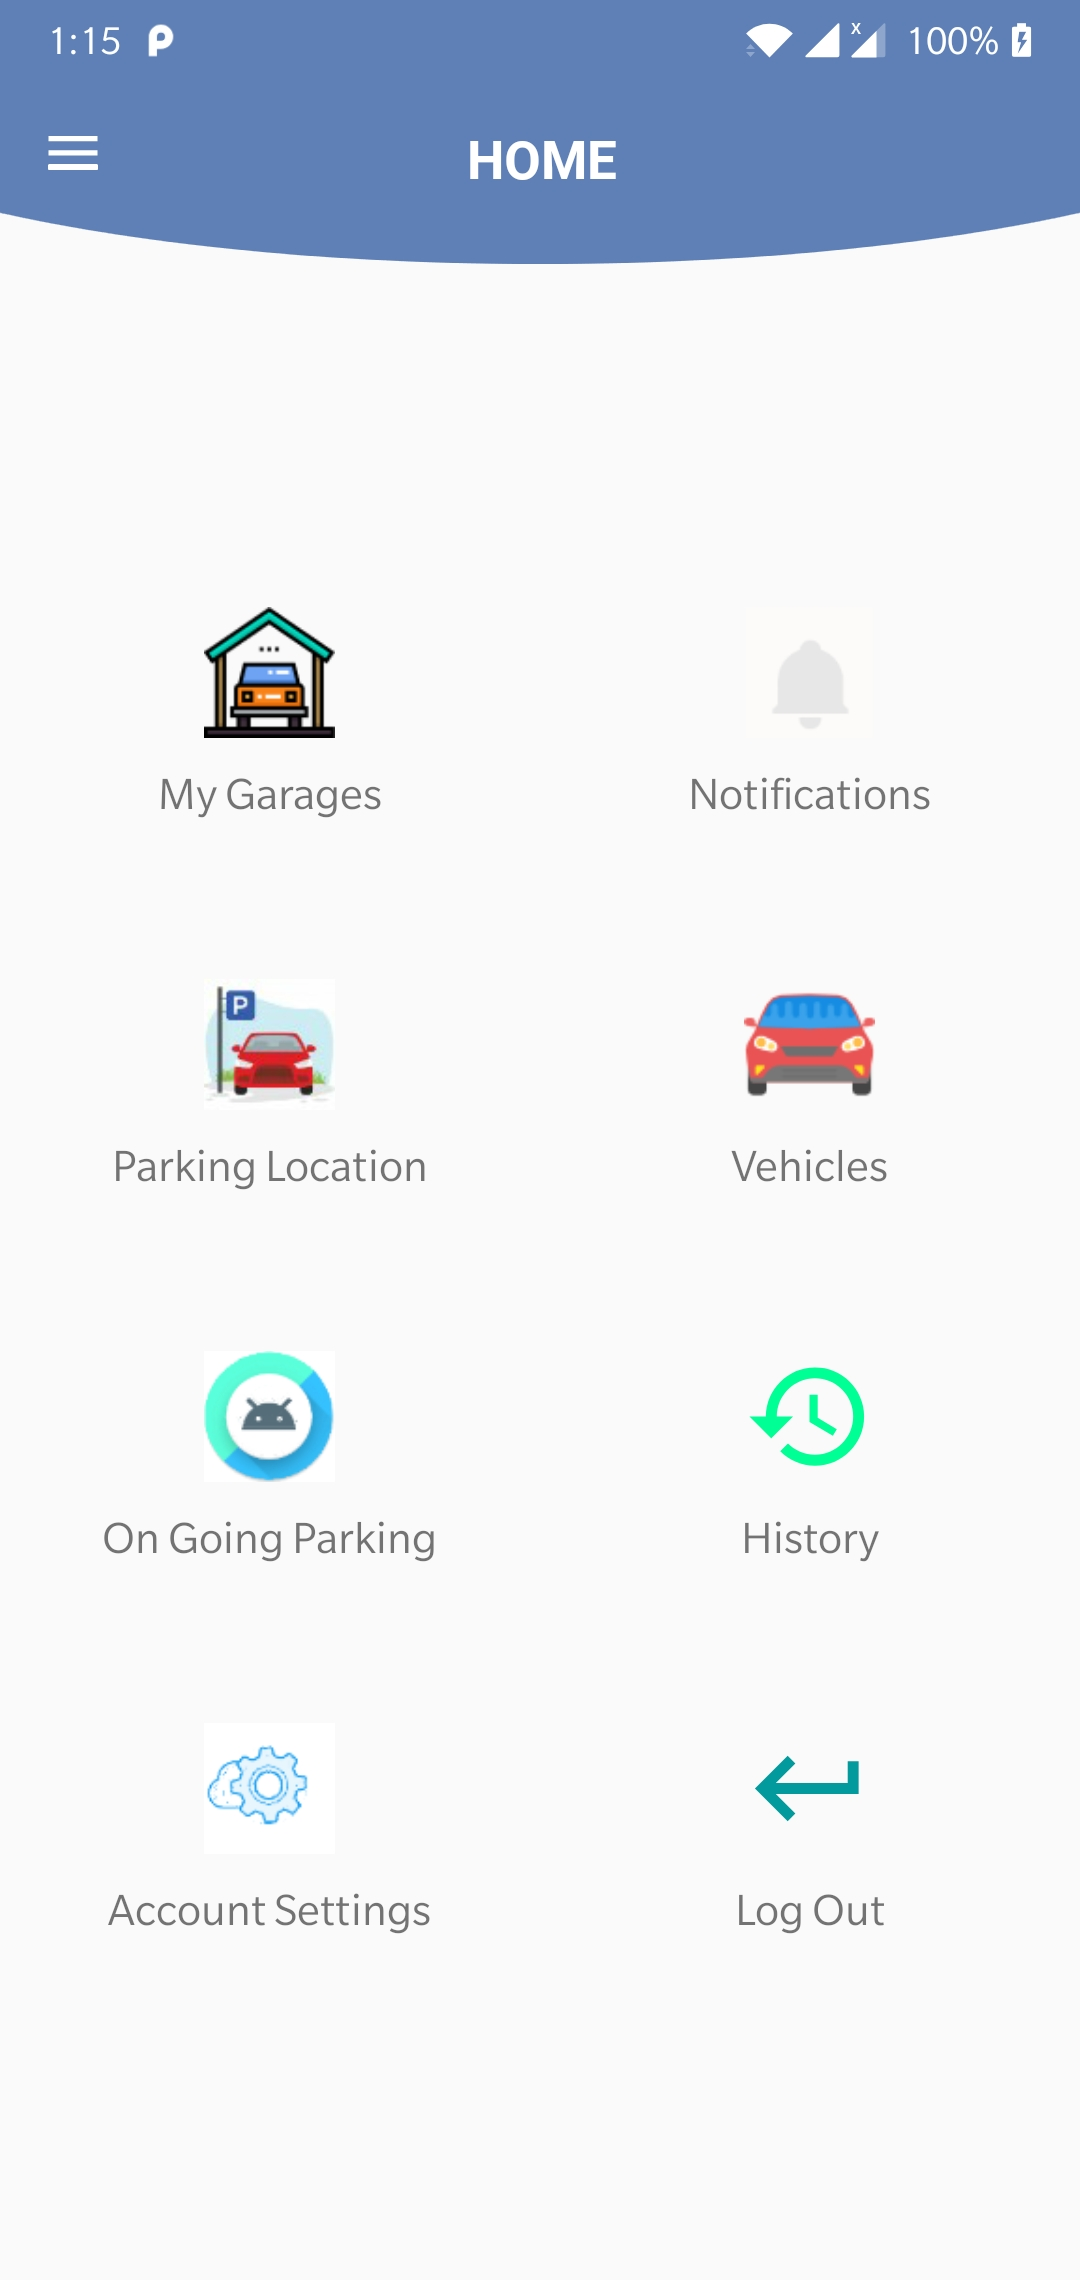
\includegraphics[width=\linewidth]{HomeActivity.jpg}
        \label{arch50}
        \caption{Home window}
    \end{subfigure}
    \label{fig:arp_os}
\end{figure}

\subsubsection{Vehicle Details}
A user can enter vehicles he wishes to park in vehicle window.
\begin{figure}[h!]
        \begin{minipage}[b]{1\linewidth}
        \centering
        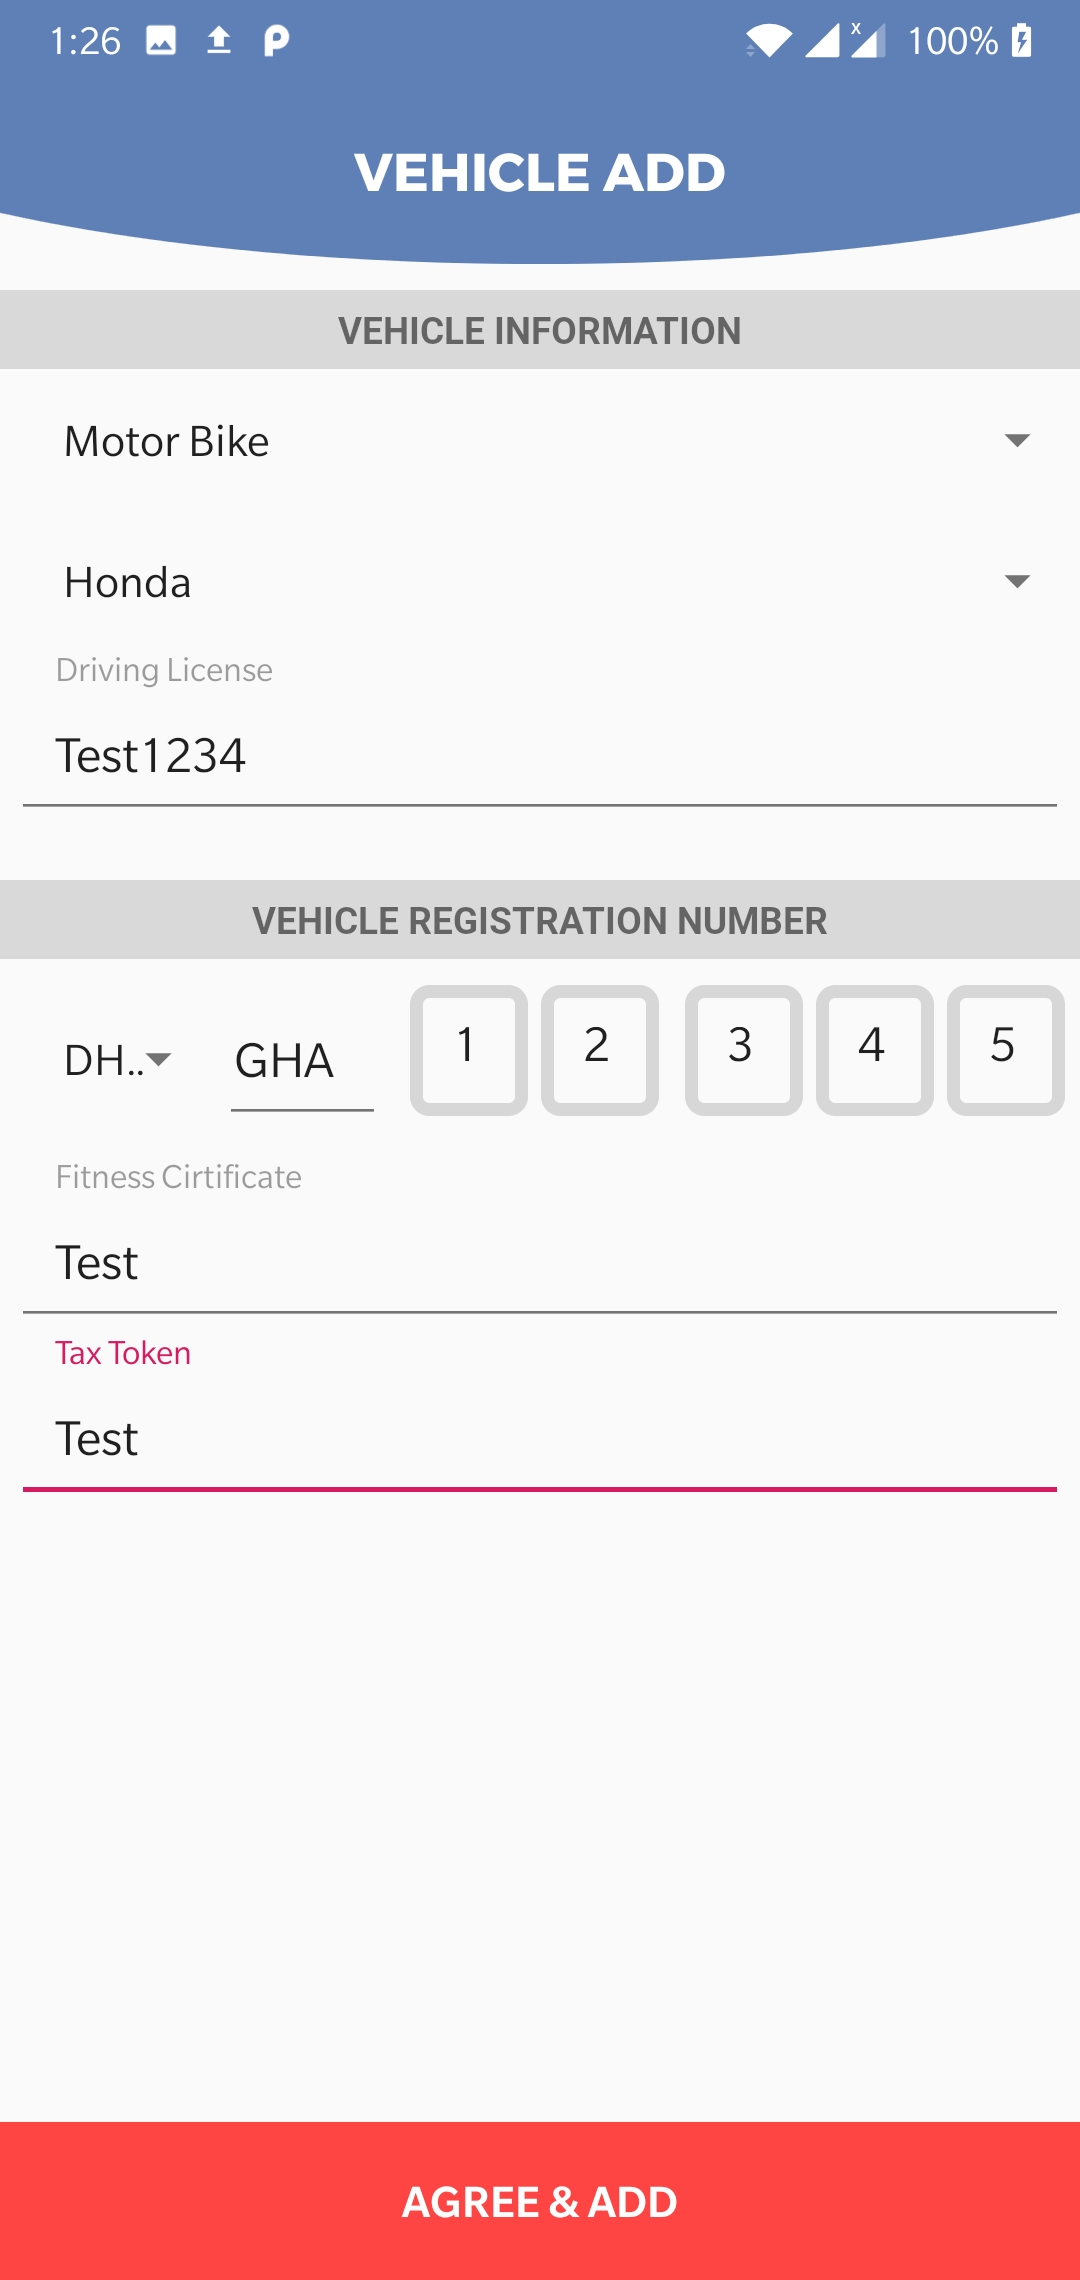
\includegraphics[width=6cm]{Vehicle/VehicleEditActivity_used_for_adding_vehicle.jpg}
        \label{arch6}
        \caption{Vehicle Add Window}
        \end{minipage}
\end{figure}
\begin{figure}[h!]
        \begin{minipage}[b]{1\linewidth}
        \centering
        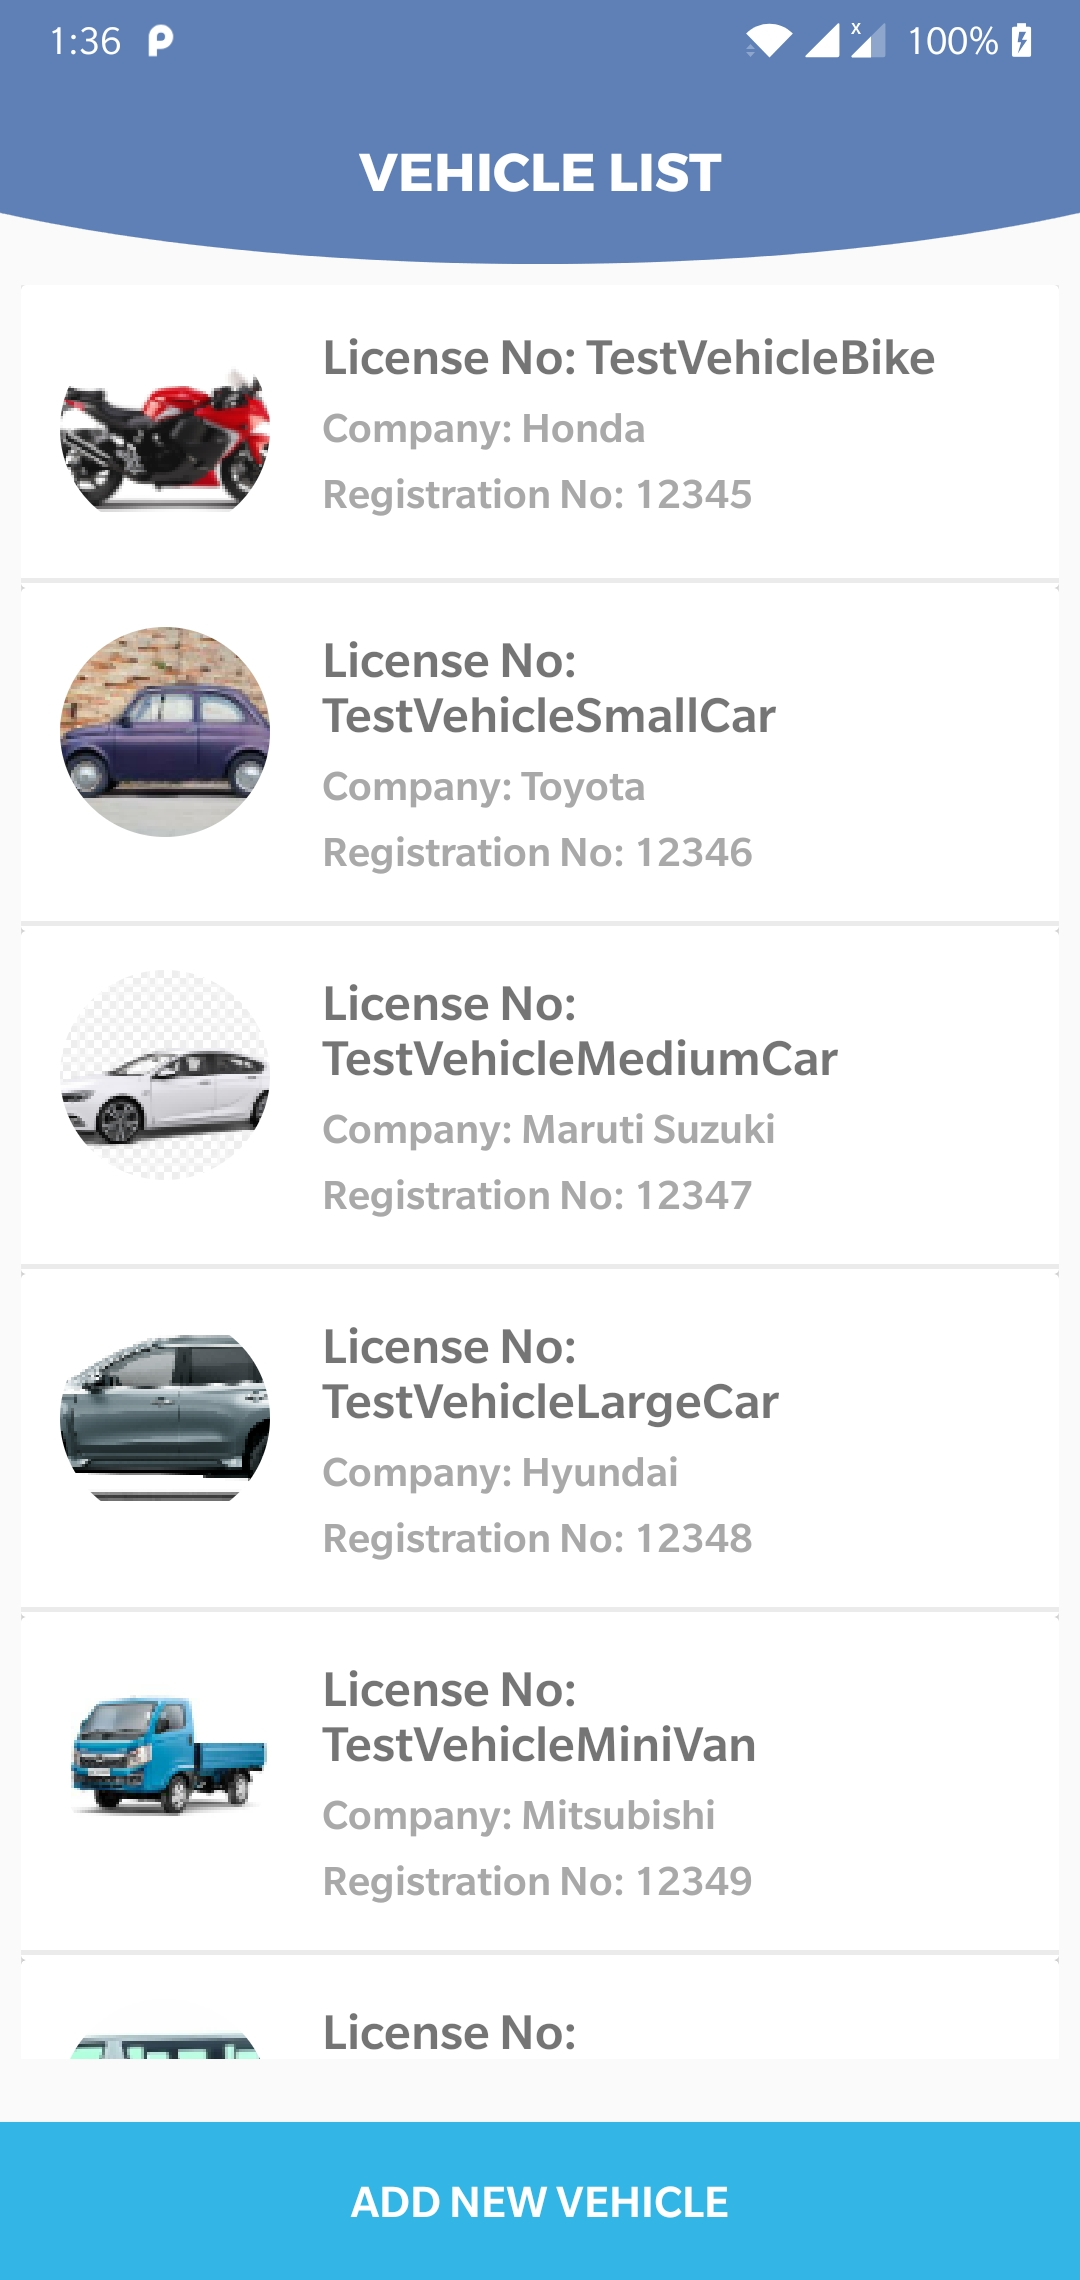
\includegraphics[width=6cm]{Vehicle/Vehicle_List_after_adding_all_types_of_vehicles.jpg}
        \label{arch5}
        \caption{Vehicle List Window}
        \end{minipage}
\end{figure}
\subsubsection{Adding Garage as Renter}
User's single registered account provides him services of both as the customer and the renter.He can add garage and provide garage spaces for rent in a specified time-interval.To rent spaces, detials of spaces have to be inserted and all records will be stored in the server side database.User can also deactivate the availabilty of his rented space for a certain period and activate then with new initialized date.While adding garage, a record for the user is created as renter and this record will be stored in the database.
\newpage
\begin{figure}[h!]
        \begin{minipage}[b]{1\linewidth}
        \centering
        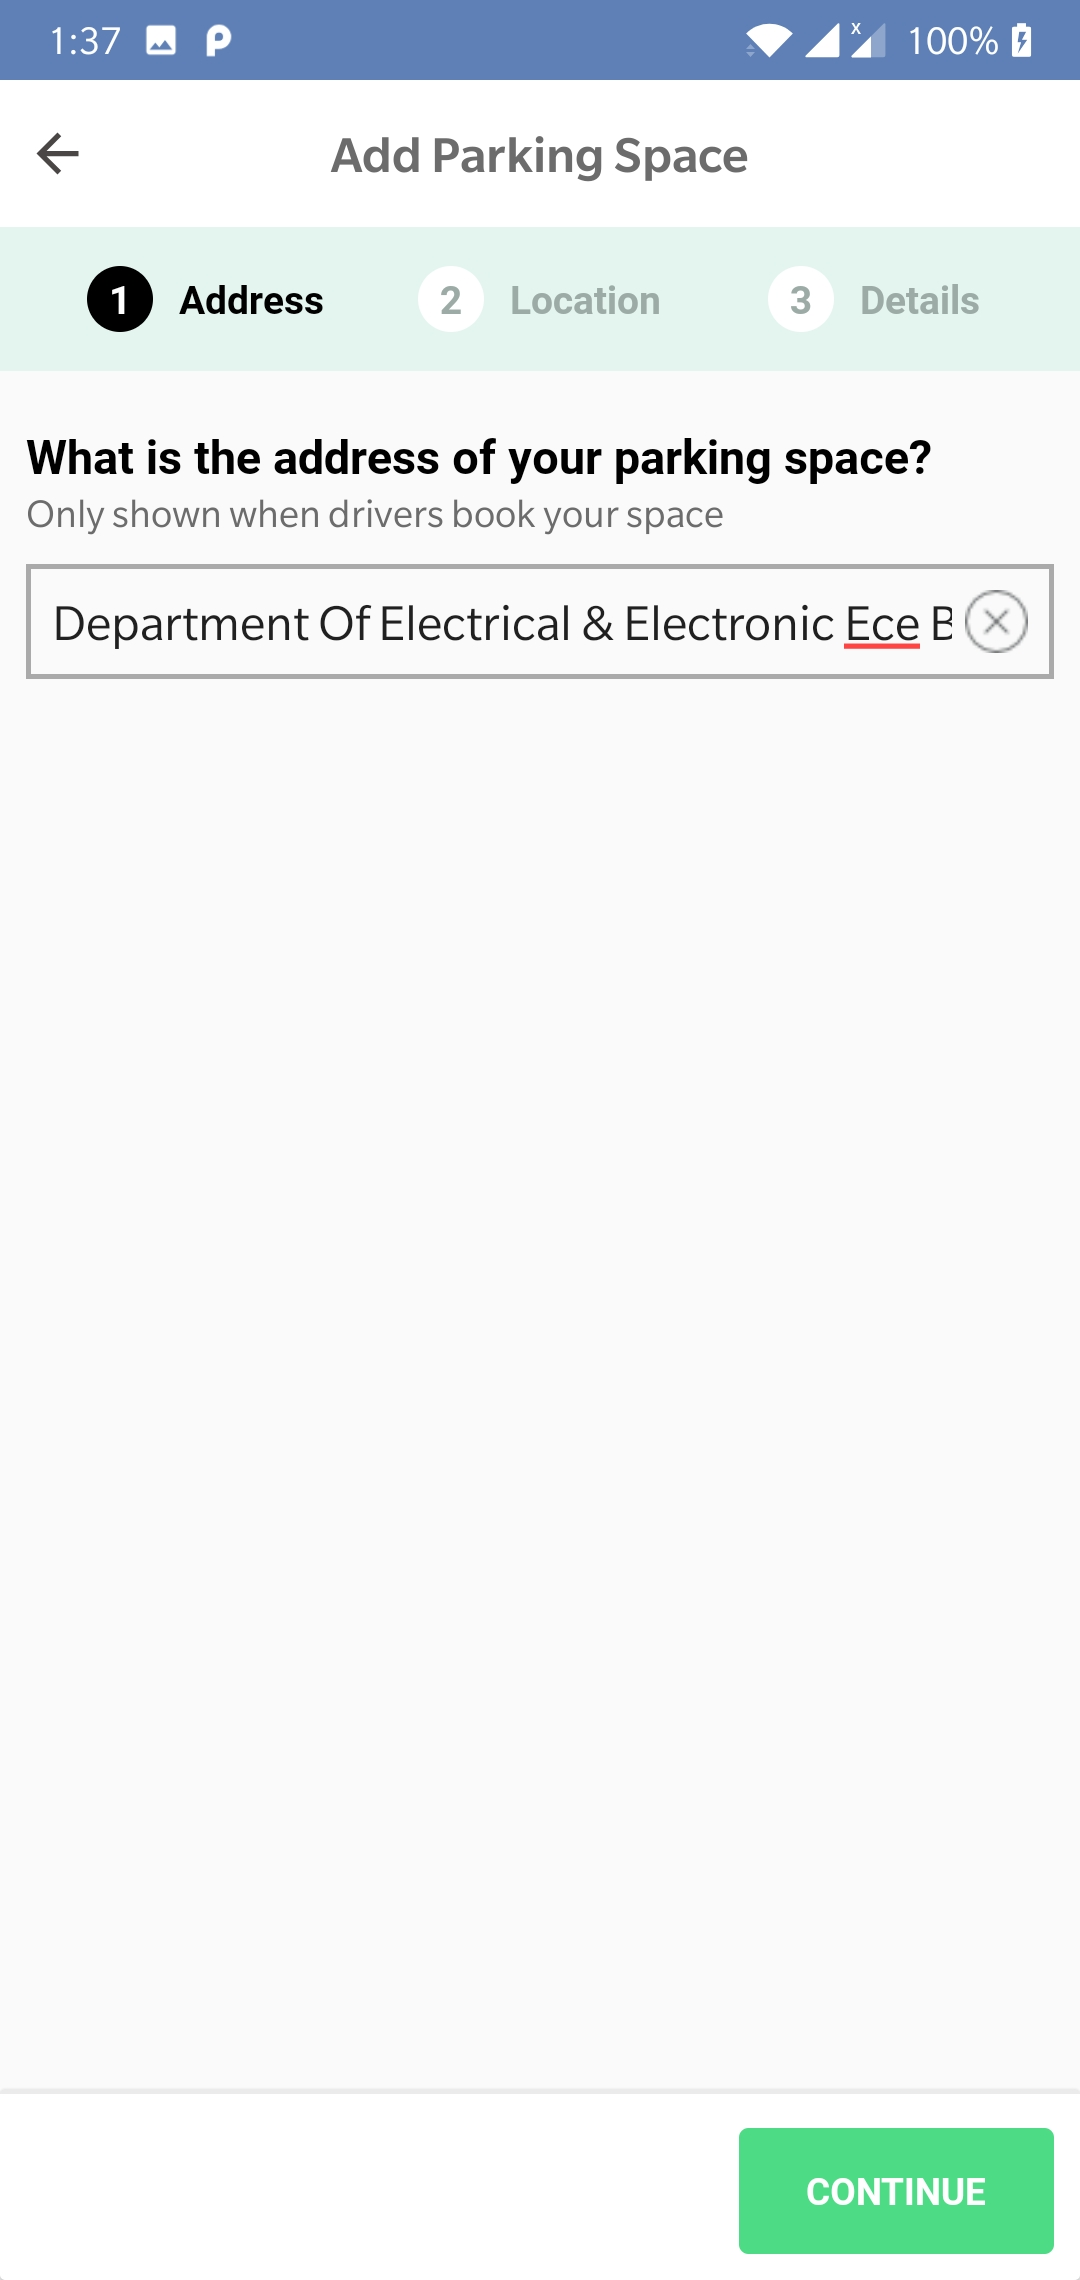
\includegraphics[width=6cm]{GarageAdd/AddressFragment1.jpg}
        \label{arch6}
        \caption{Garage Add Search}
        \end{minipage}
\end{figure}
\begin{figure}[h!]
        \begin{minipage}[b]{1\linewidth}
        \centering
        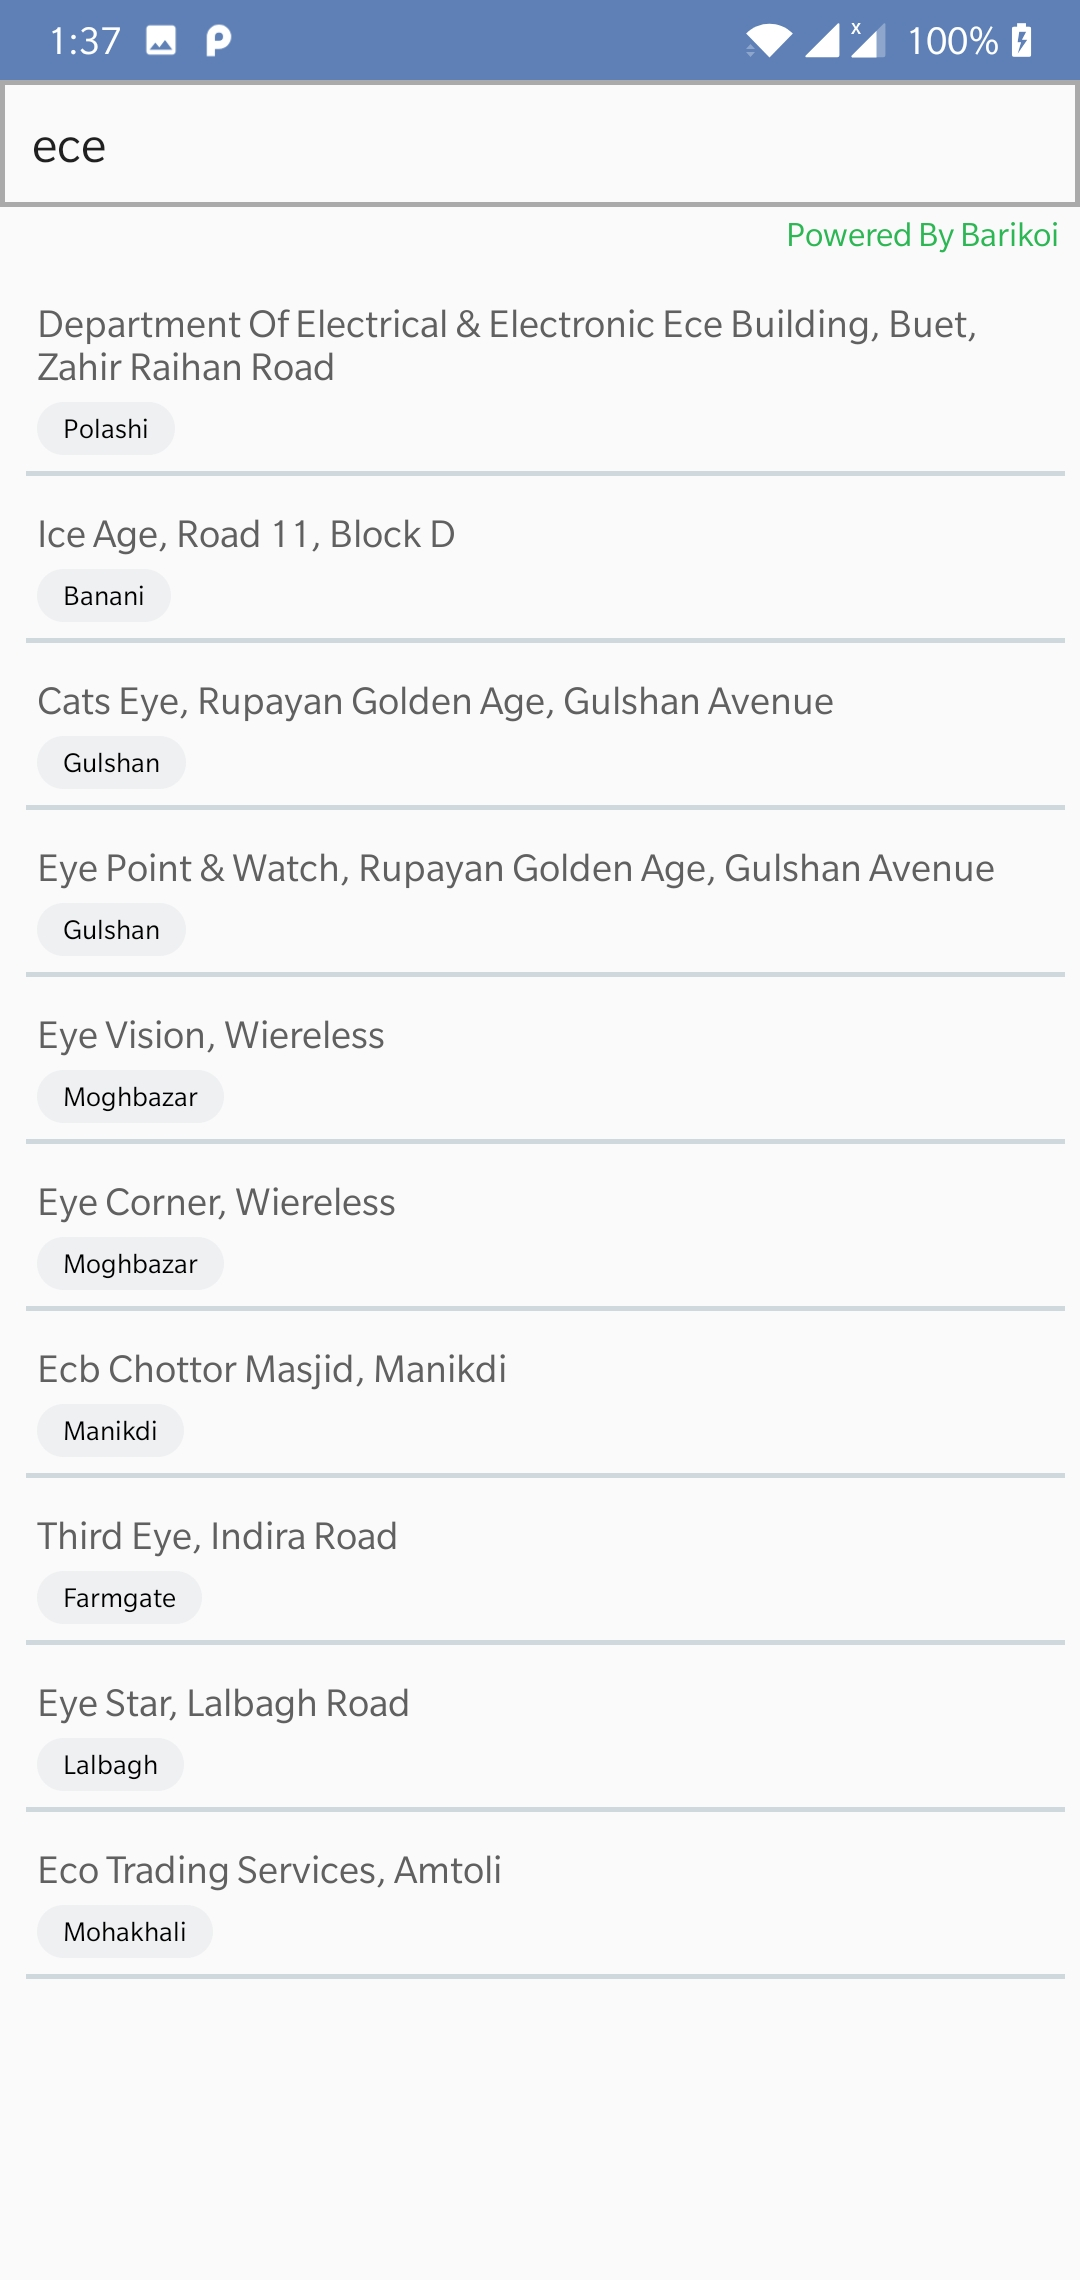
\includegraphics[width=6cm]{GarageAdd/AddressFragment2.jpg}
        \label{arch7}
        \caption{Garage Add Search Suggestions}
        \end{minipage}
\end{figure}
\newpage
\begin{figure}[h!]
        \begin{minipage}[b]{1\linewidth}
        \centering
        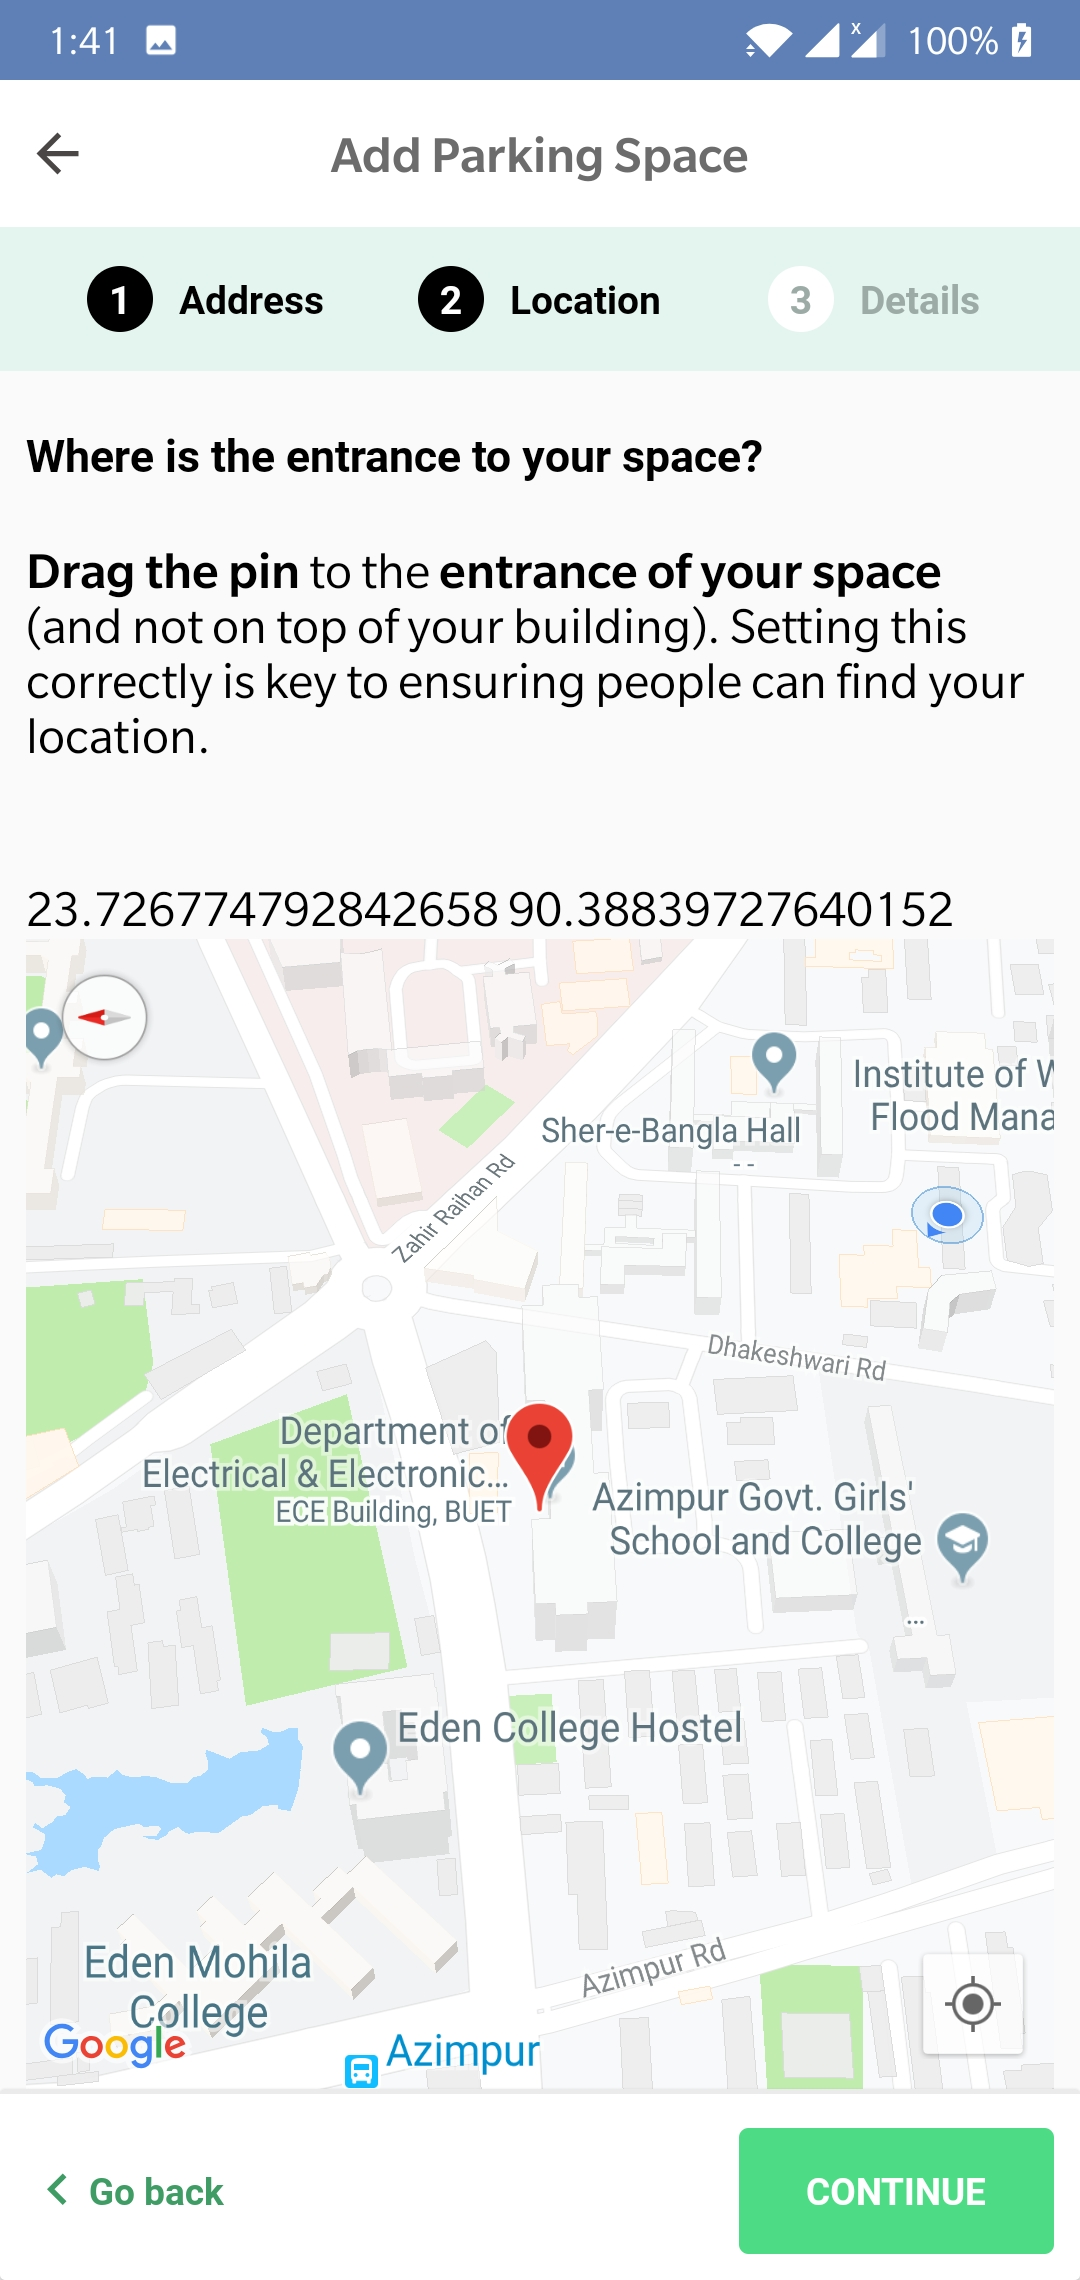
\includegraphics[width=6cm]{GarageAdd/Location.jpg}
        \label{arch8}
        \caption{Garage Add Location Map}
        \end{minipage}
\end{figure}
\begin{figure}[h!]
        \begin{minipage}[b]{1\linewidth}
        \centering
        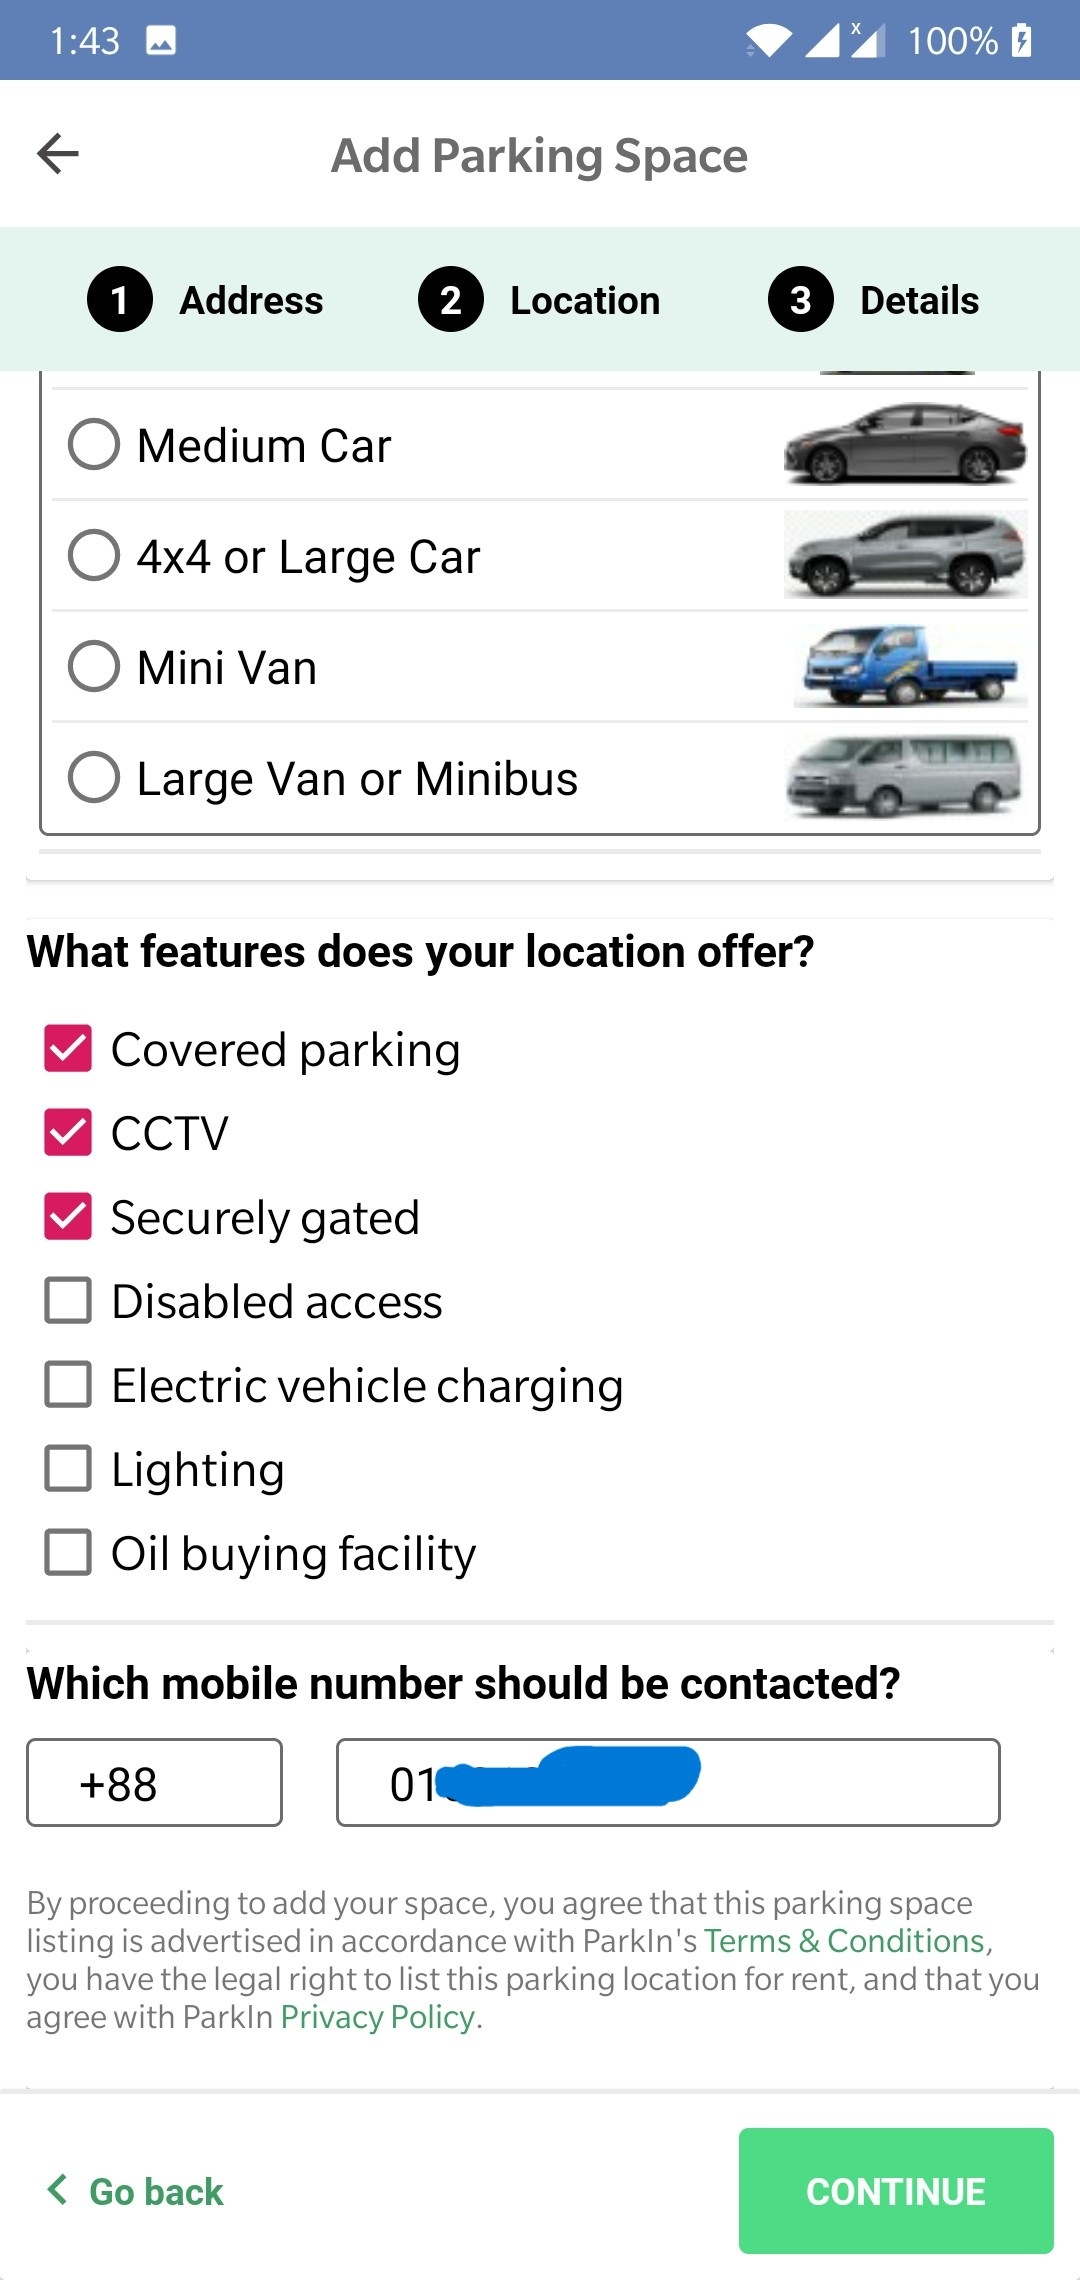
\includegraphics[width=6cm]{GarageAdd/DetailsFragment1.jpg}
        \label{arch9}
        \caption{Garage Add details Start time End time}
        \end{minipage}
\end{figure}
\begin{figure}[h!]
        \begin{minipage}[b]{1\linewidth}
        \centering
        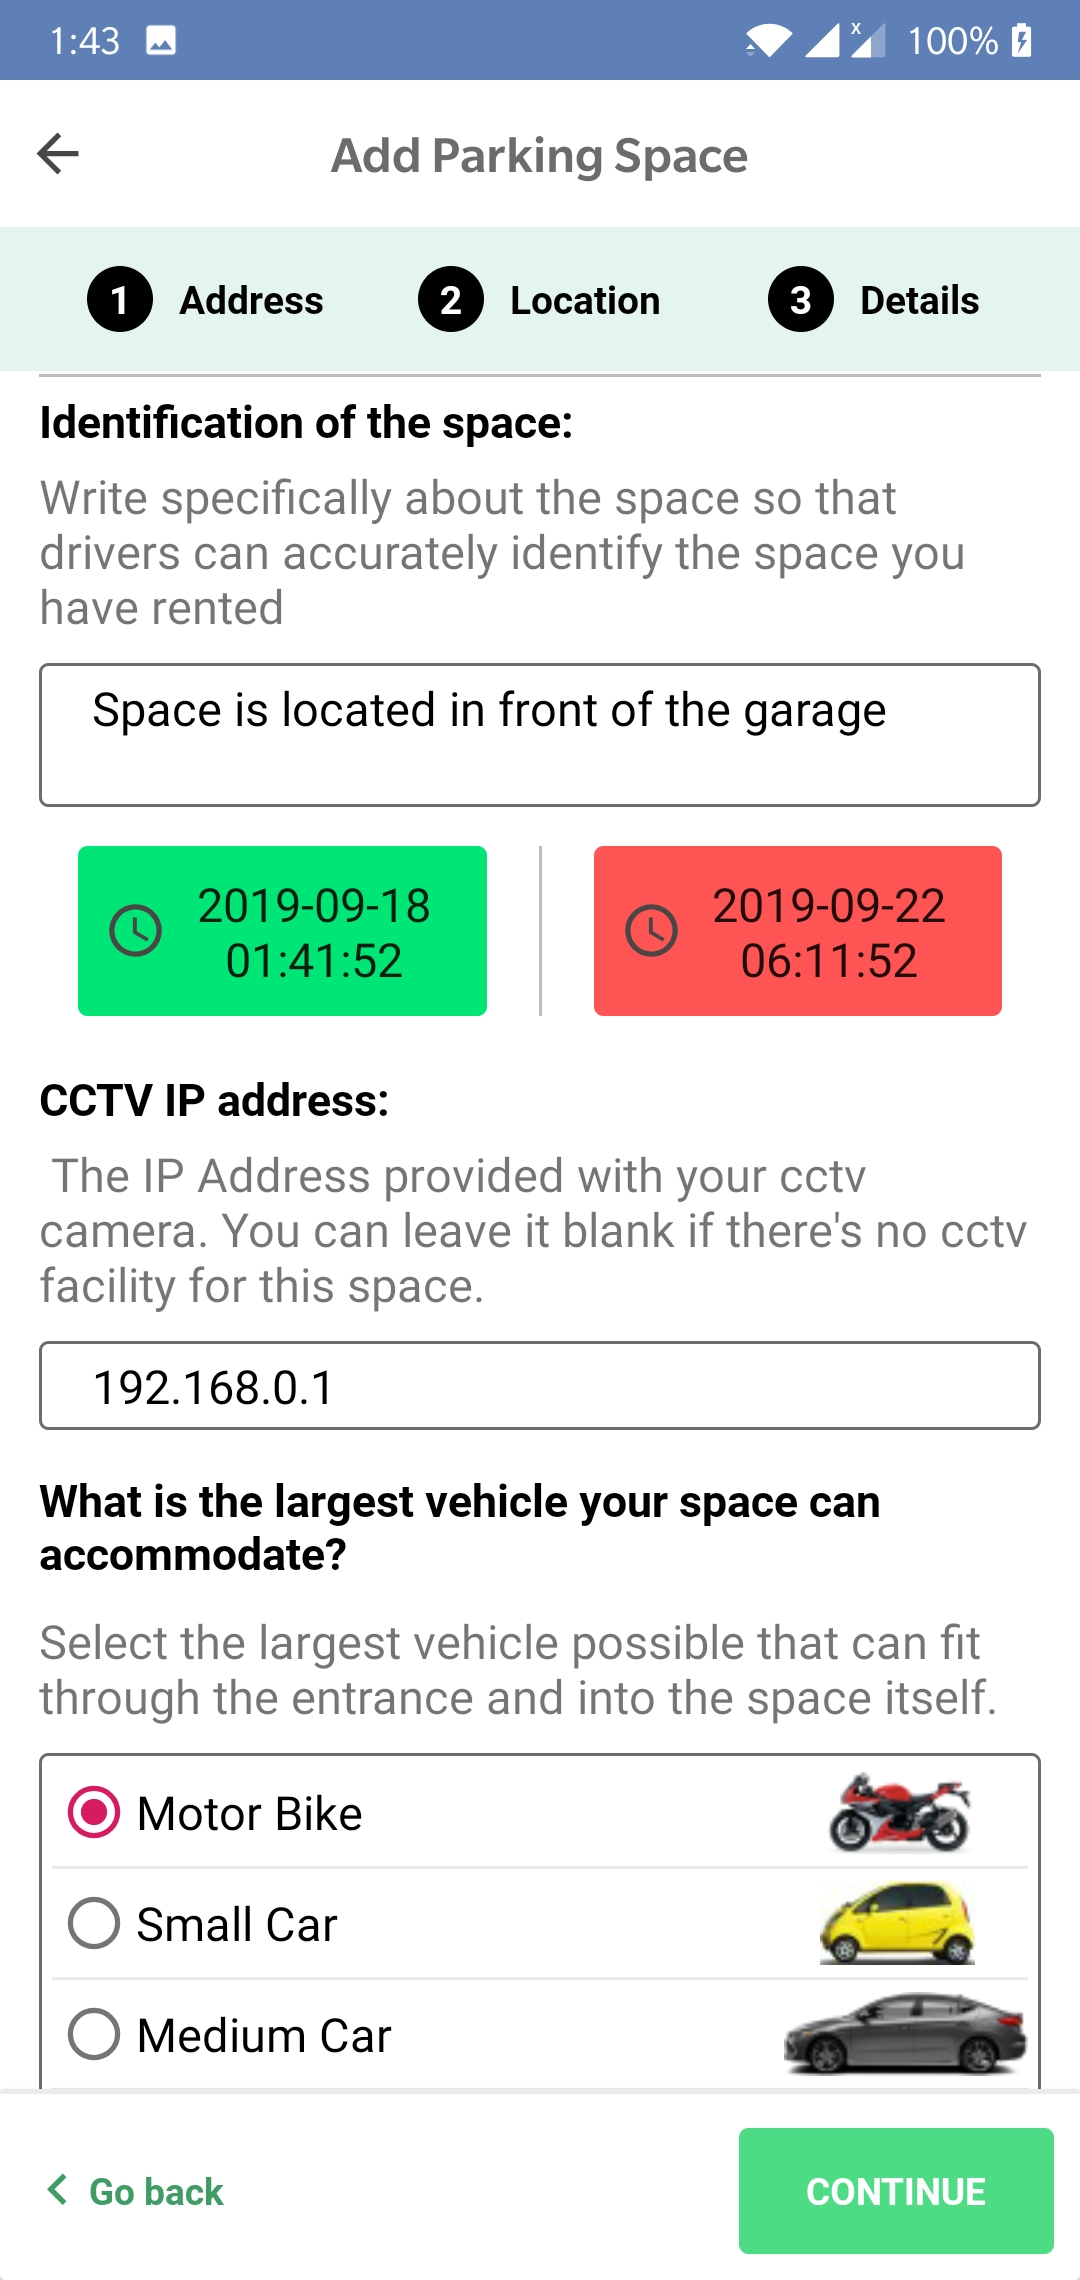
\includegraphics[width=6cm]{GarageAdd/DetailsFragment2.jpg}
        \label{arch10}
        \caption{Garage Add details Size selection}
        \end{minipage}
\end{figure}
\newpage
\subsubsection{Location Selection for Parking}
The user selects \textbf{Parking Location Icon} for getting available garages.By selecting desired garage with Arrival and Departure time along with the vehicle type, user can see multiple spaces available for him. User has to select one of the spaces provided where he desires to park the vehicle.
\newpage
\begin{figure}[h!]
    \centering
    \begin{subfigure}[t]{0.3\textwidth}
    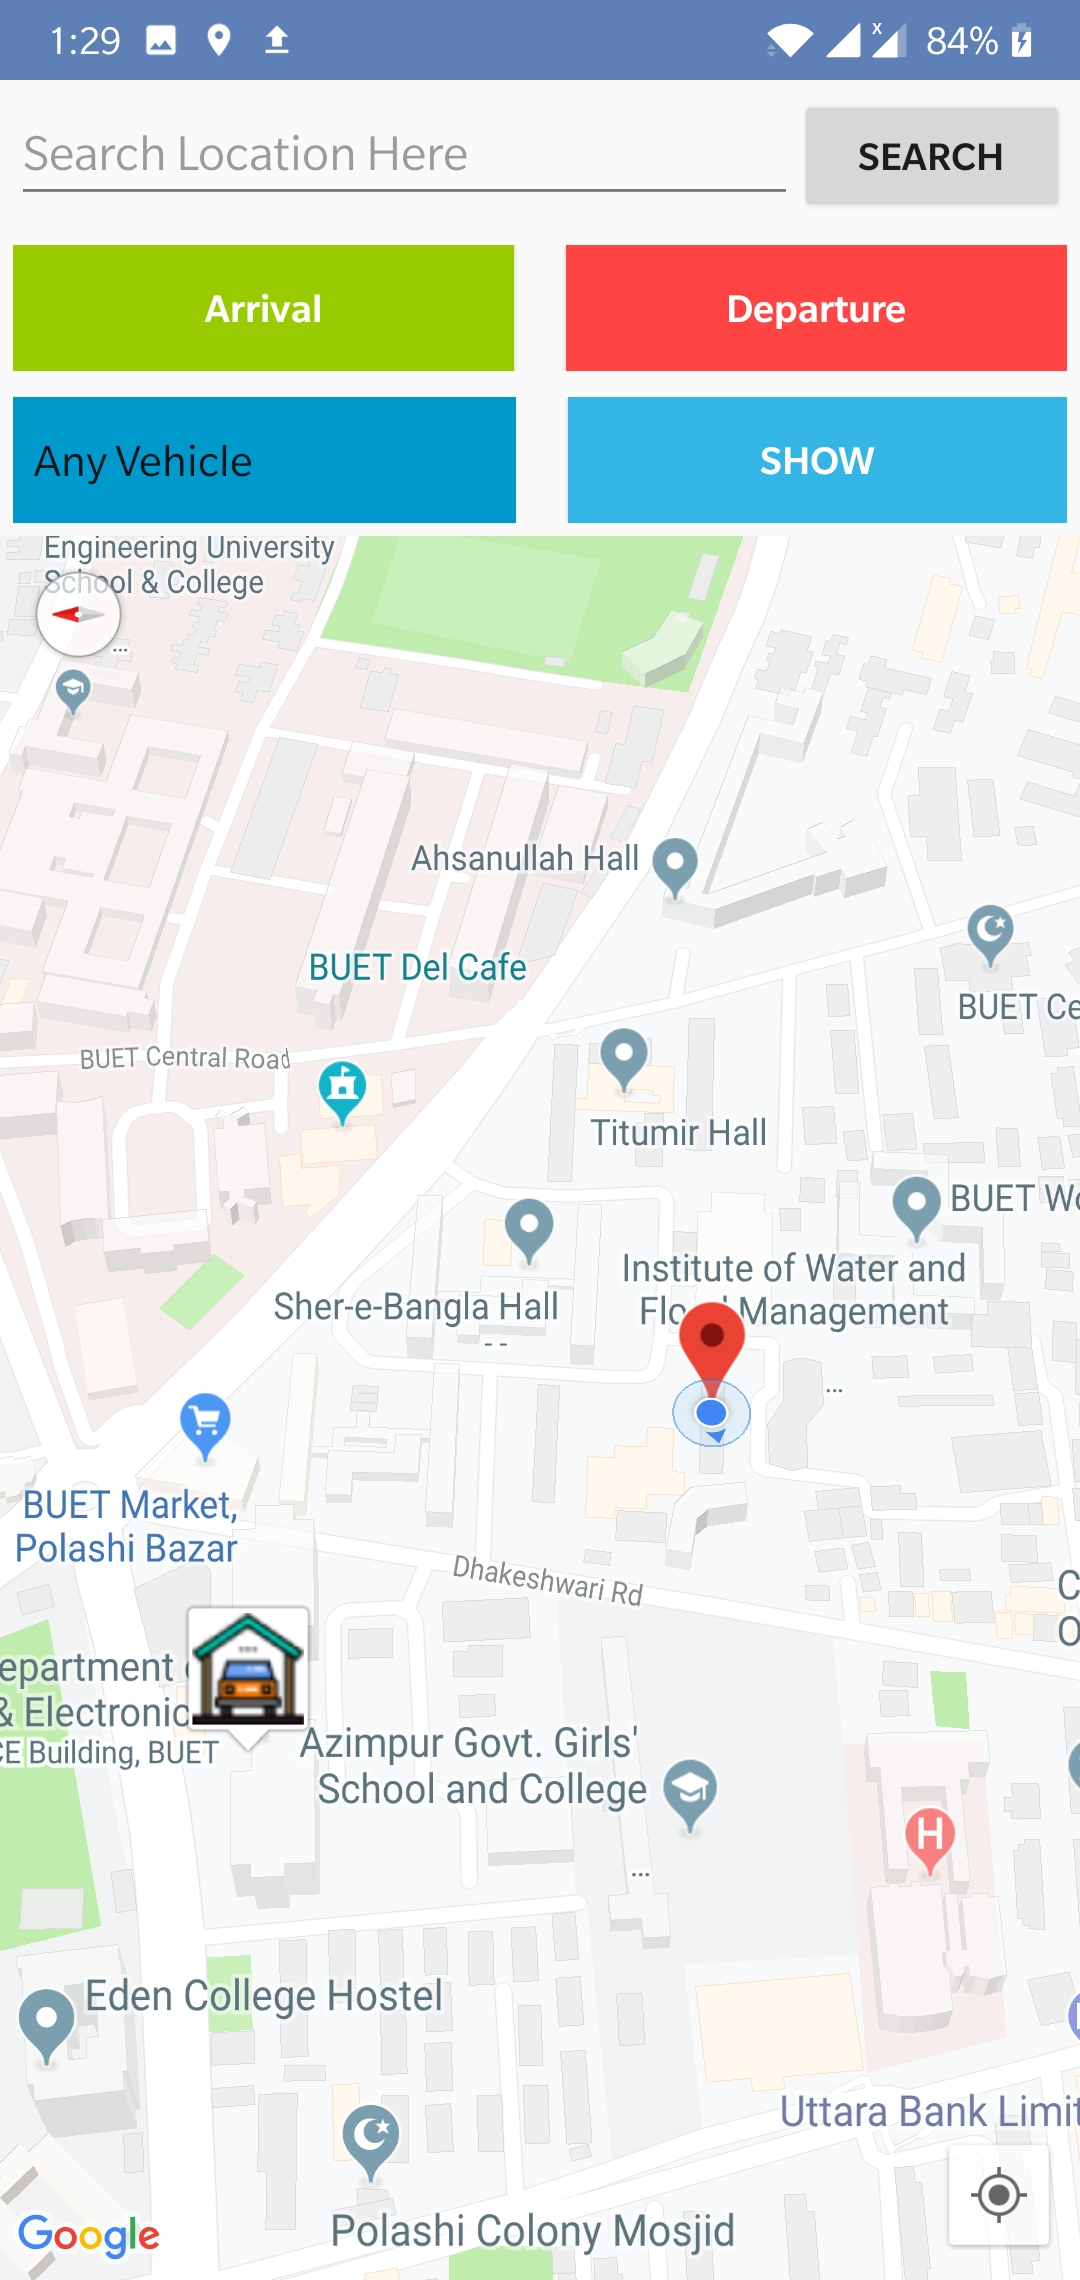
\includegraphics[width=\linewidth]{Location_Selection/search_for_parkinglocations.jpg}
        \label{arch5}
        \caption{Search Location window}
    \end{subfigure}
    \begin{subfigure}[t]{0.3\textwidth}
    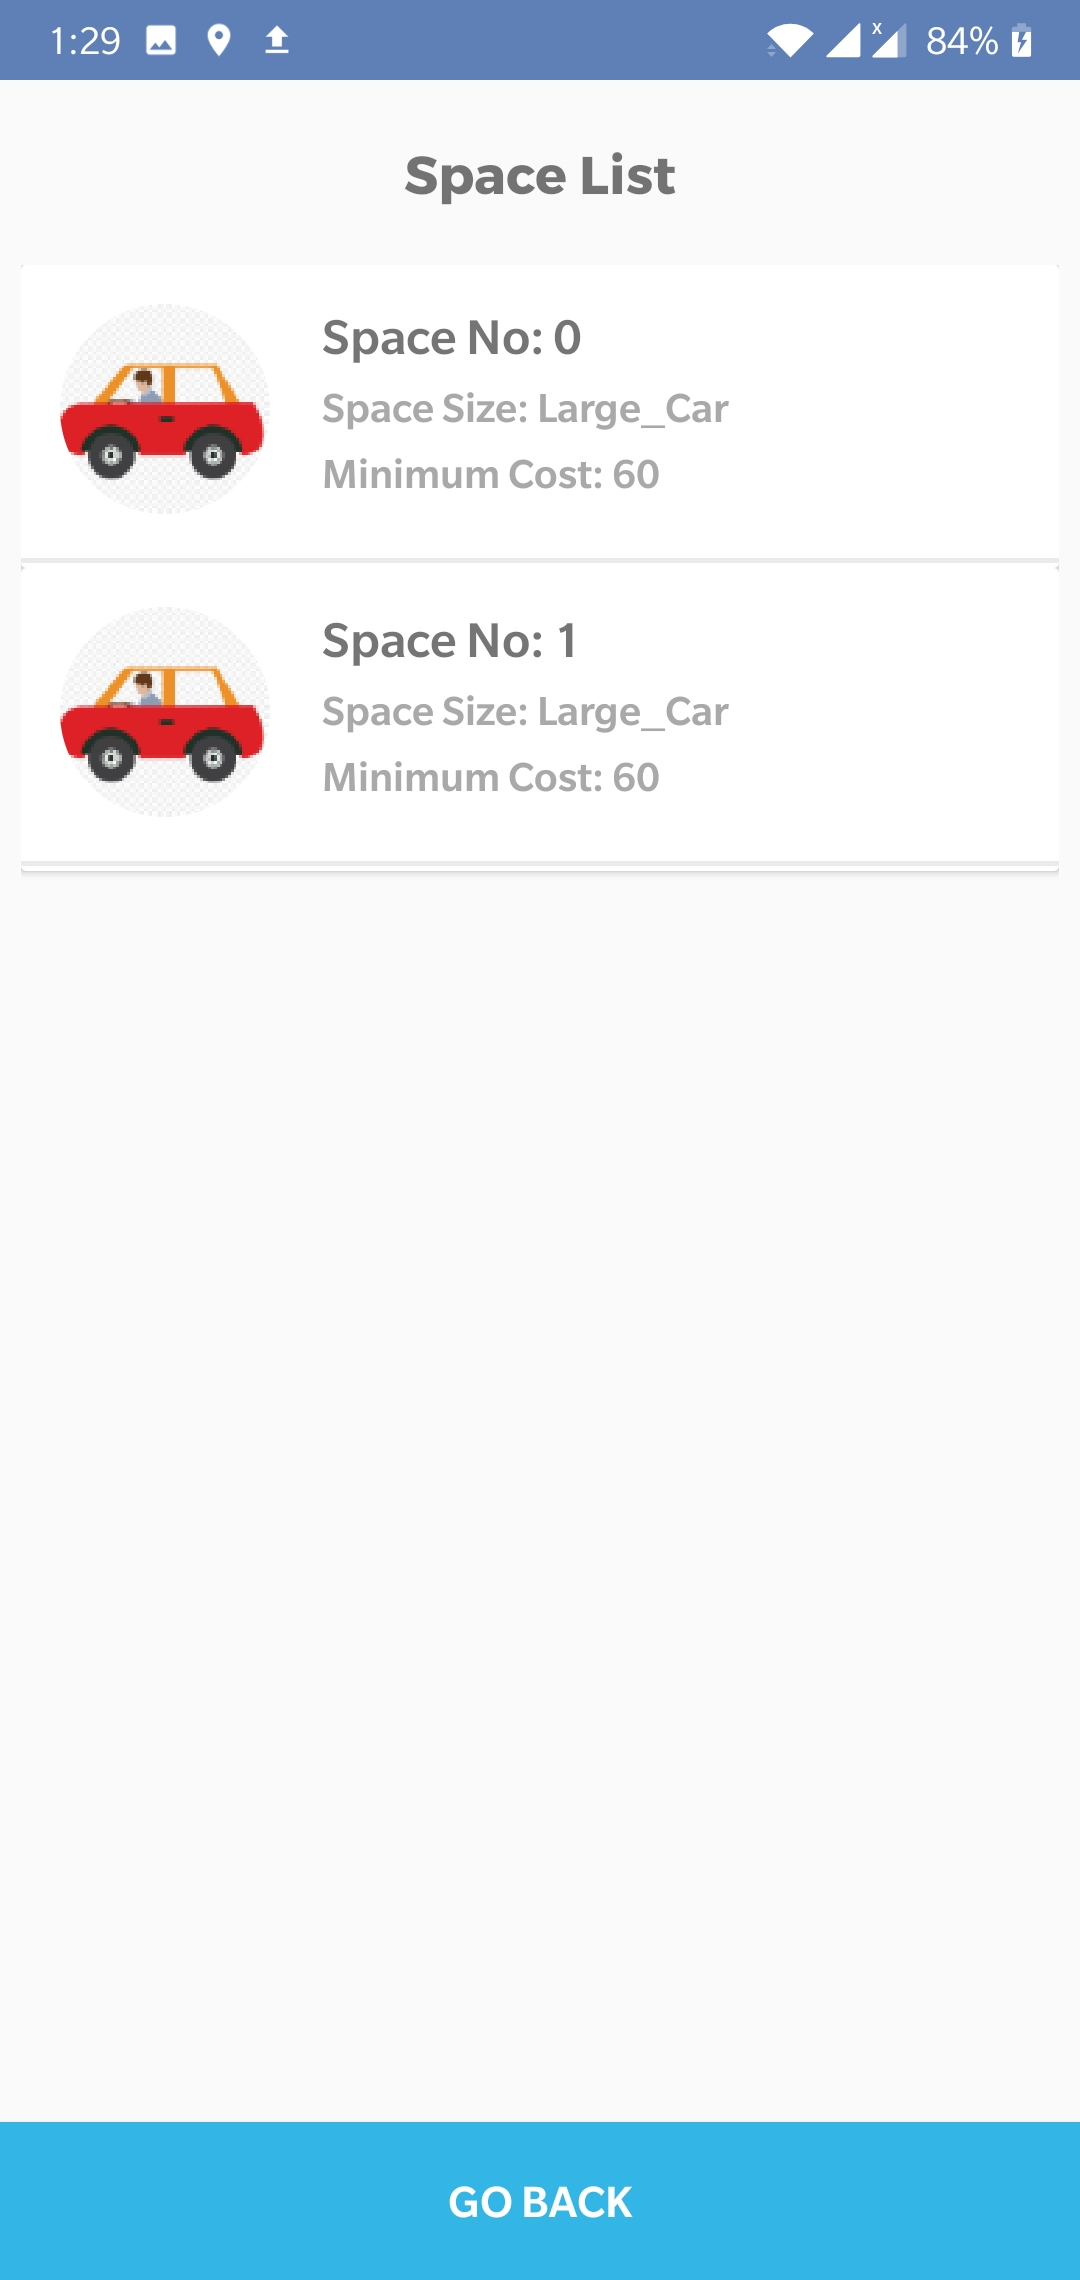
\includegraphics[width=\linewidth]{Location_Selection/showing_space_list_for_adding_vehicles.jpg}
        \label{arch50}
        \caption{Available space list}
    \end{subfigure}
    \begin{subfigure}[t]{0.3\textwidth}
    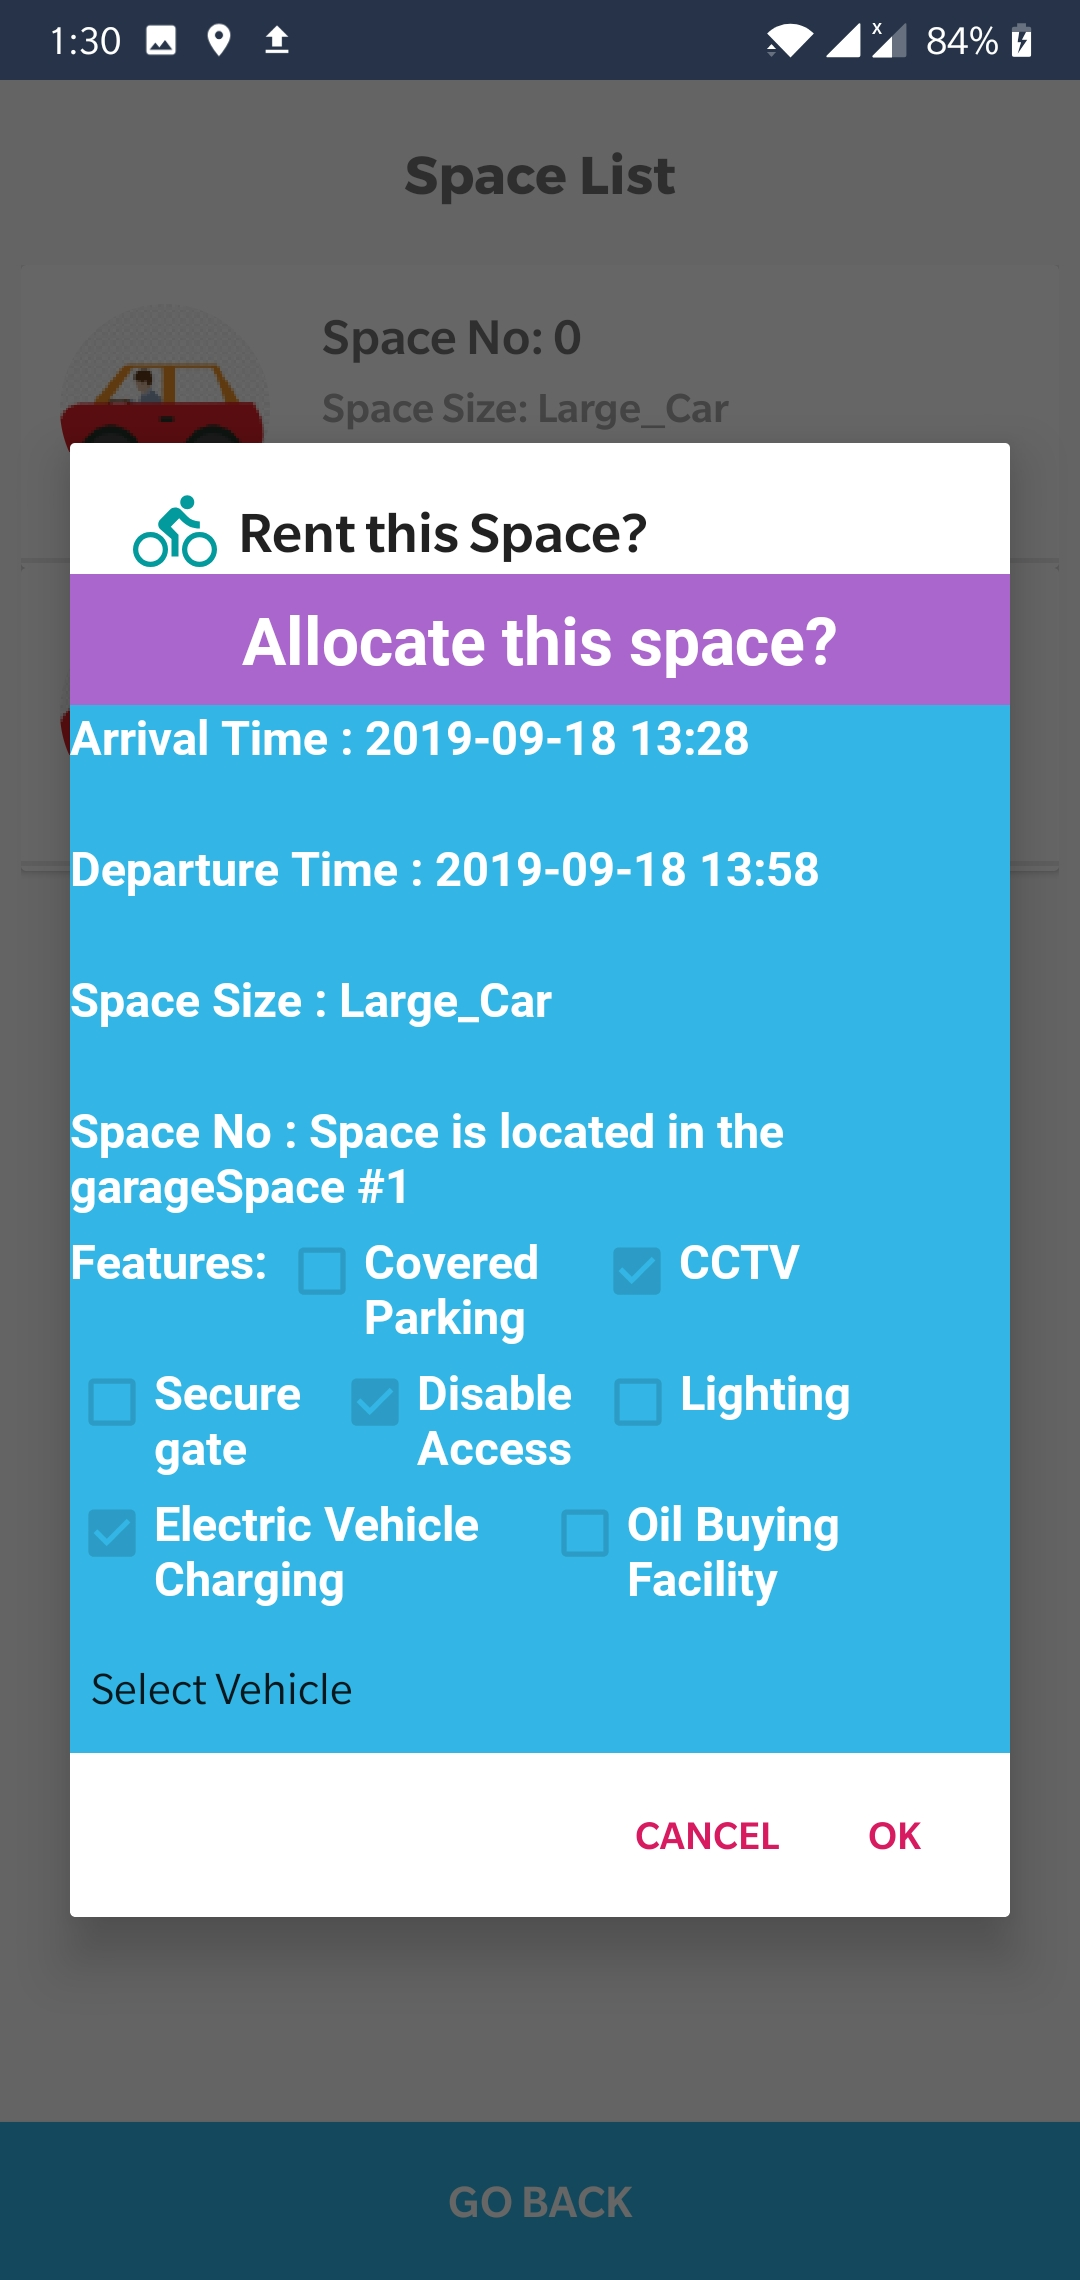
\includegraphics[width=\linewidth]{Location_Selection/select_vehicle_for_allocation.jpg}
        \label{arch50}
        \caption{Vehicle Selection}
    \end{subfigure}
    \label{fig:arp_os}
\end{figure}

\subsubsection{Notification Details}
The server sends notification to renter and client side when renting time has started and when is is over. \subsubsection{Confirmation and Payment}
When user selects slot for rent, a request is sent to the server and server responses with the confirmation status on user window.Also,Server sends notification to the user with details information about the pre-booking of slot.When user 

\begin{figure}[h!]
    \centering
    \begin{subfigure}[t]{0.4\textwidth}
    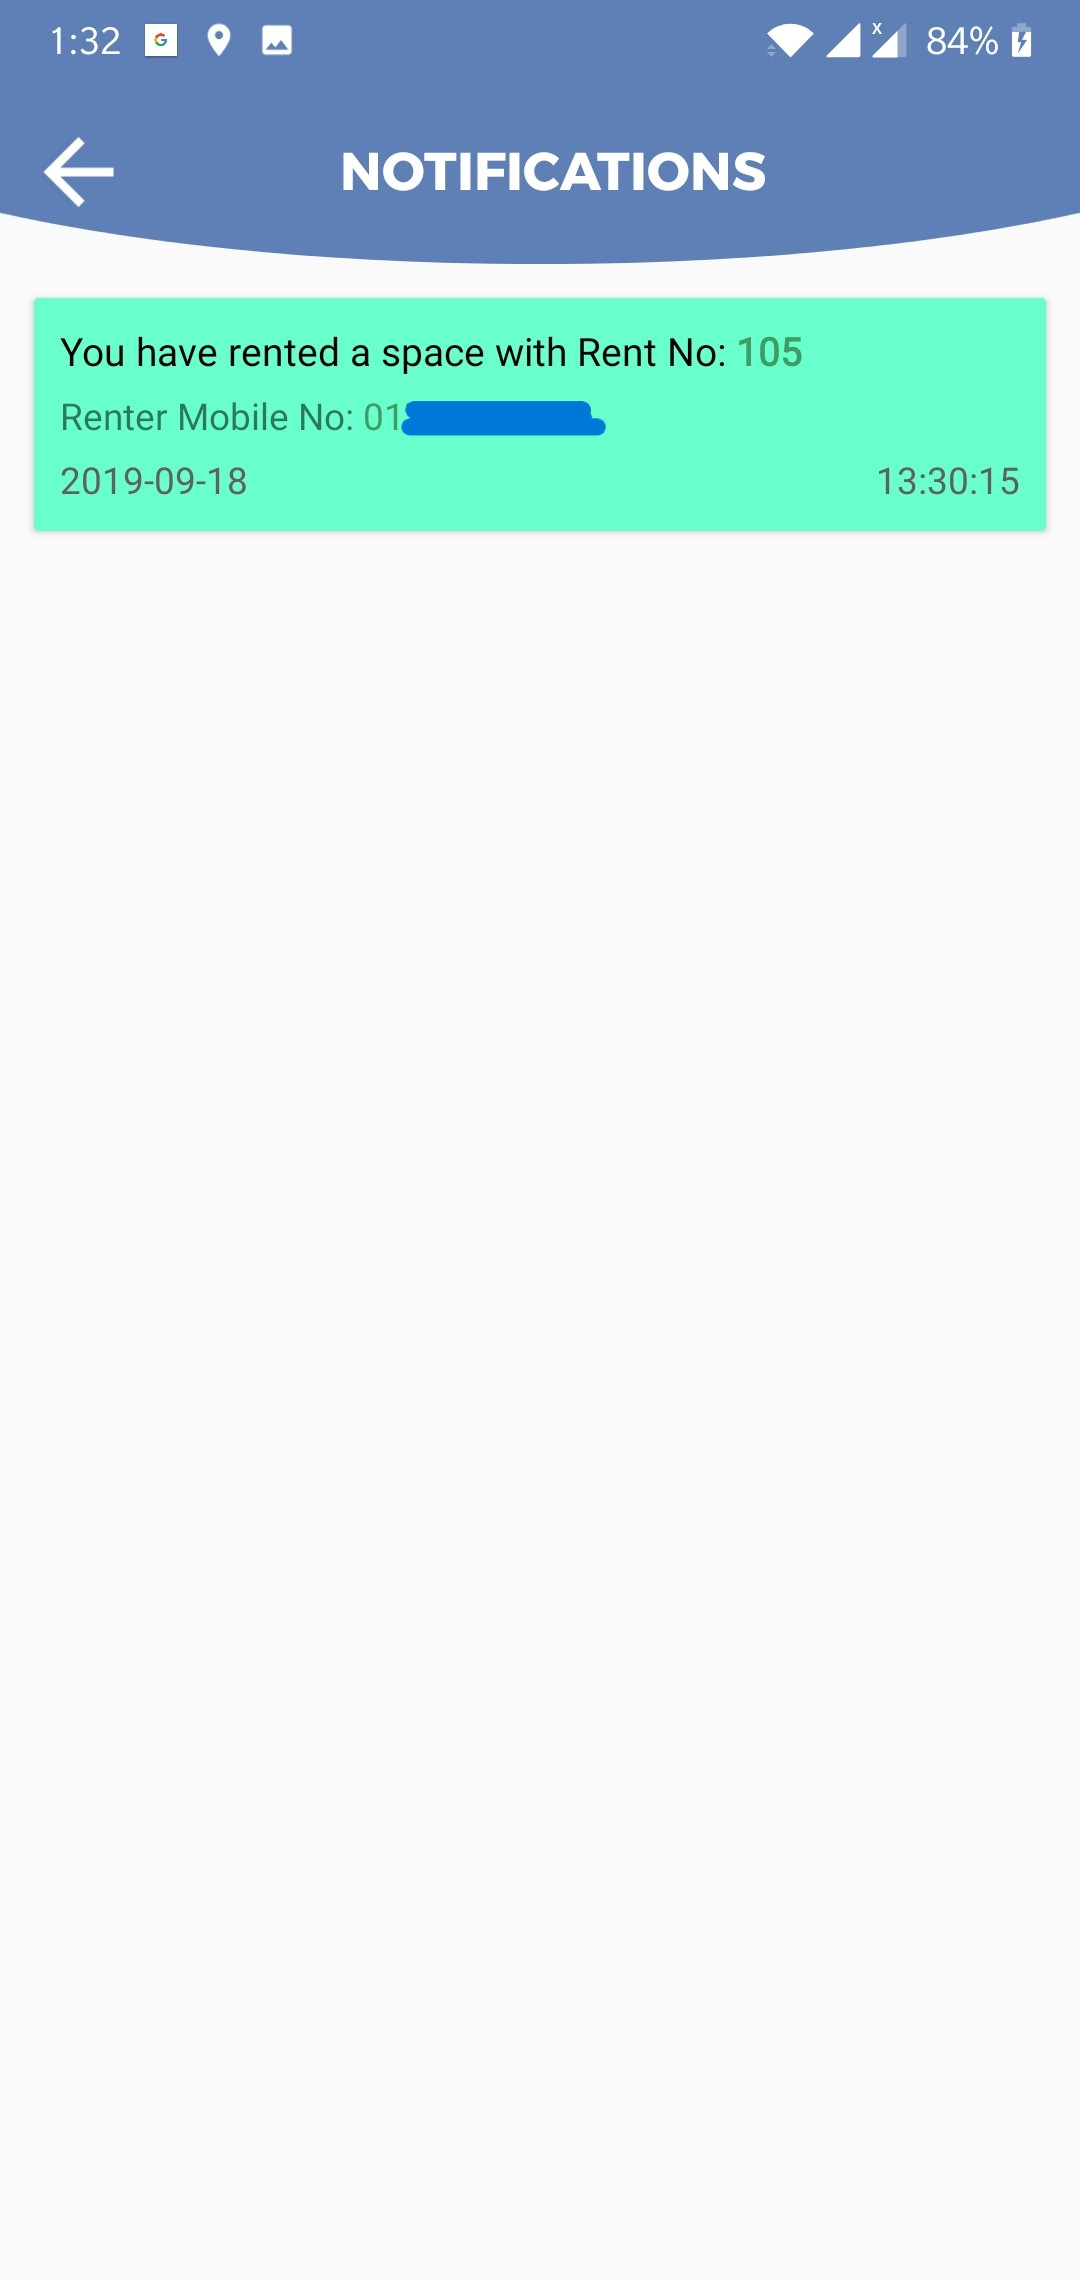
\includegraphics[width=\linewidth]{Notification/notification_showing.jpg}
        \label{arch5}
        \caption{List of Notifications}
    \end{subfigure}
    \begin{subfigure}[t]{0.4\textwidth}
    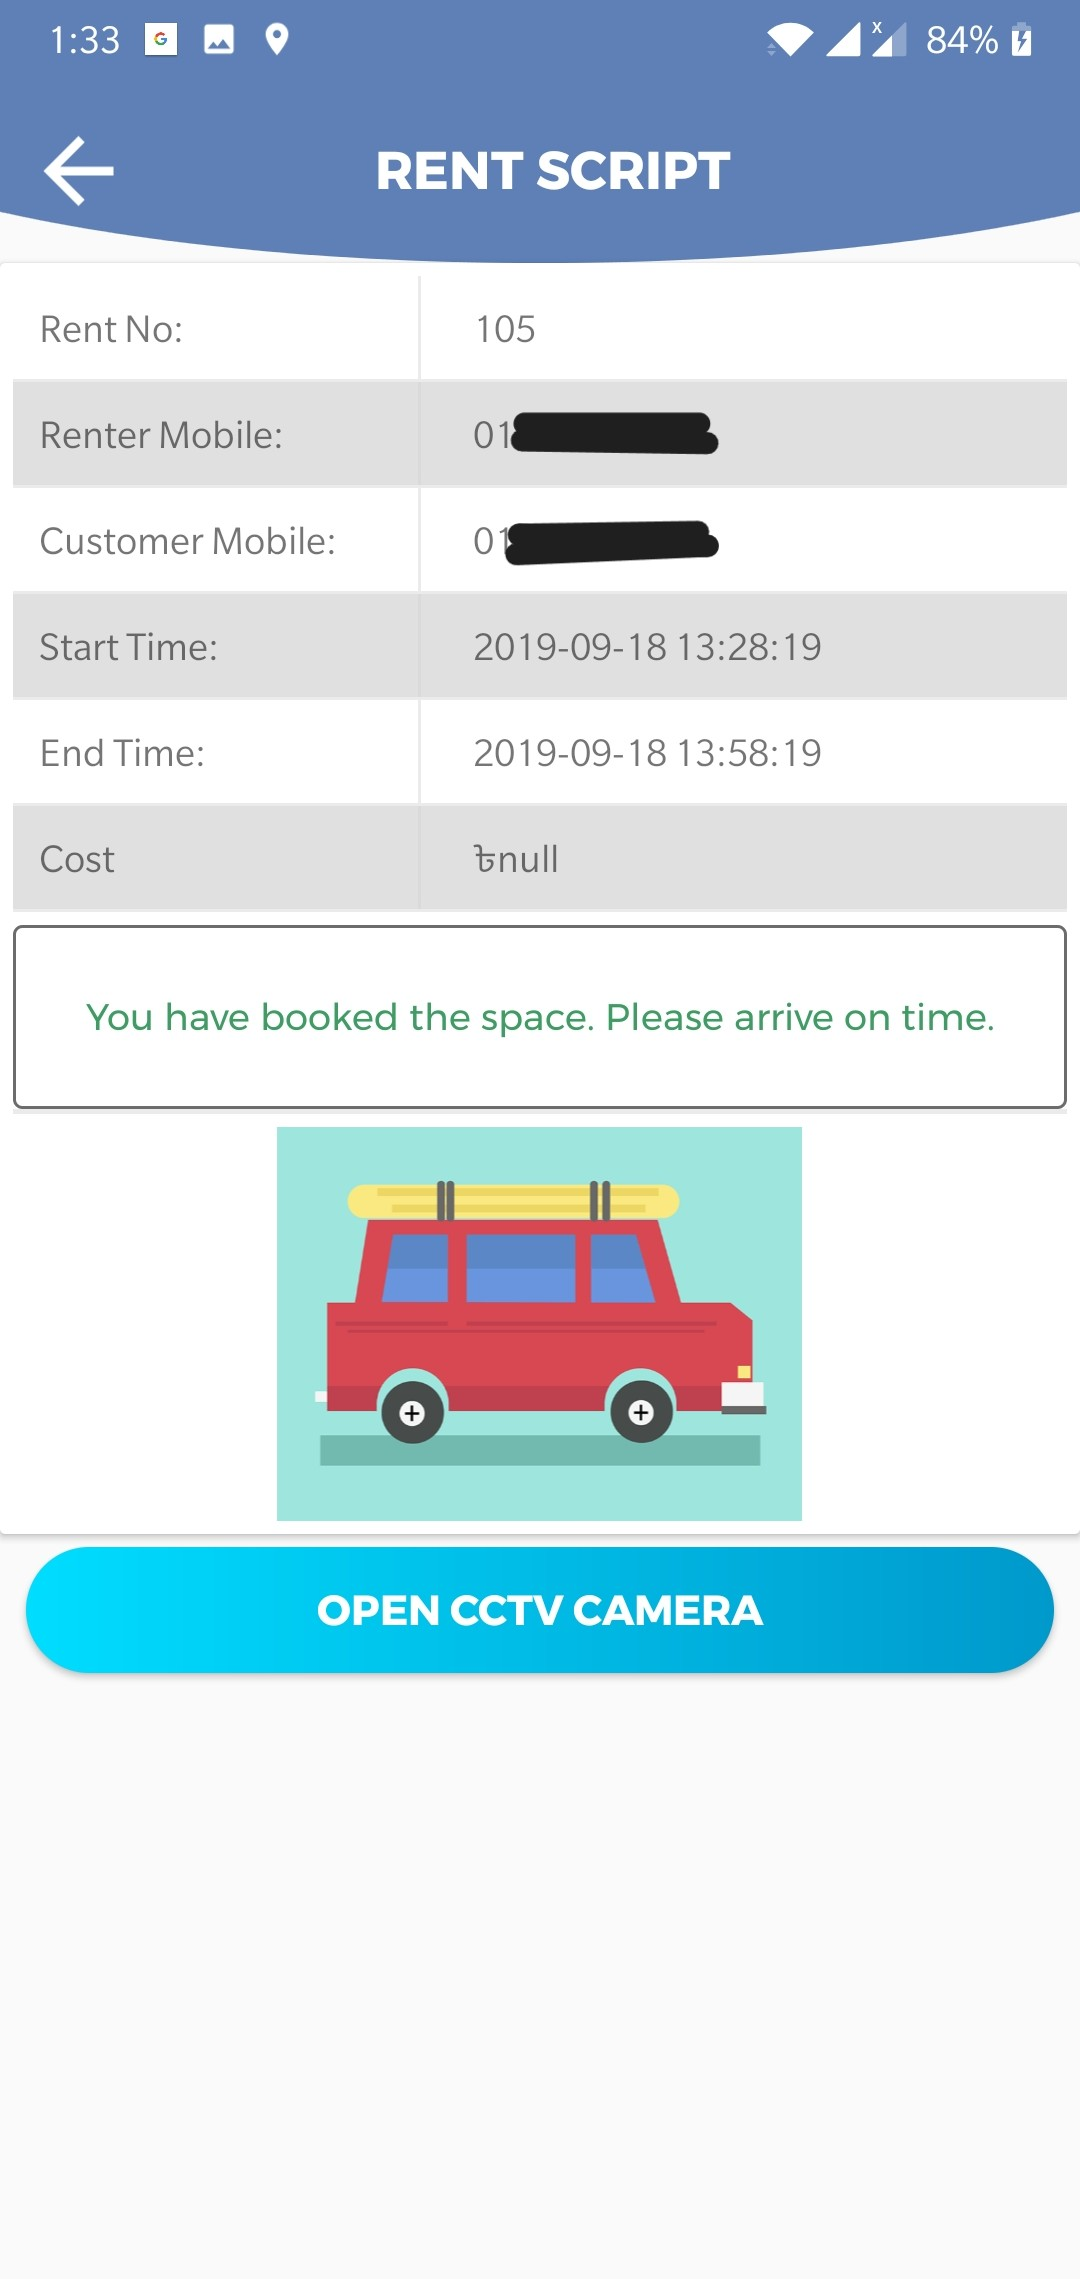
\includegraphics[width=\linewidth]{Notification/notification.jpg}
        \label{arch50}
        \caption{Single Notification Shown}
    \end{subfigure}
    \label{fig:arp_os}
\end{figure}
\subsection{Confirmation and Payment}
User will have to confirm his payment. Thus our payment window has payment methods. Then the service will be completed.
\begin{figure}[h!]
    \centering
    \begin{subfigure}[t]{0.4\textwidth}
    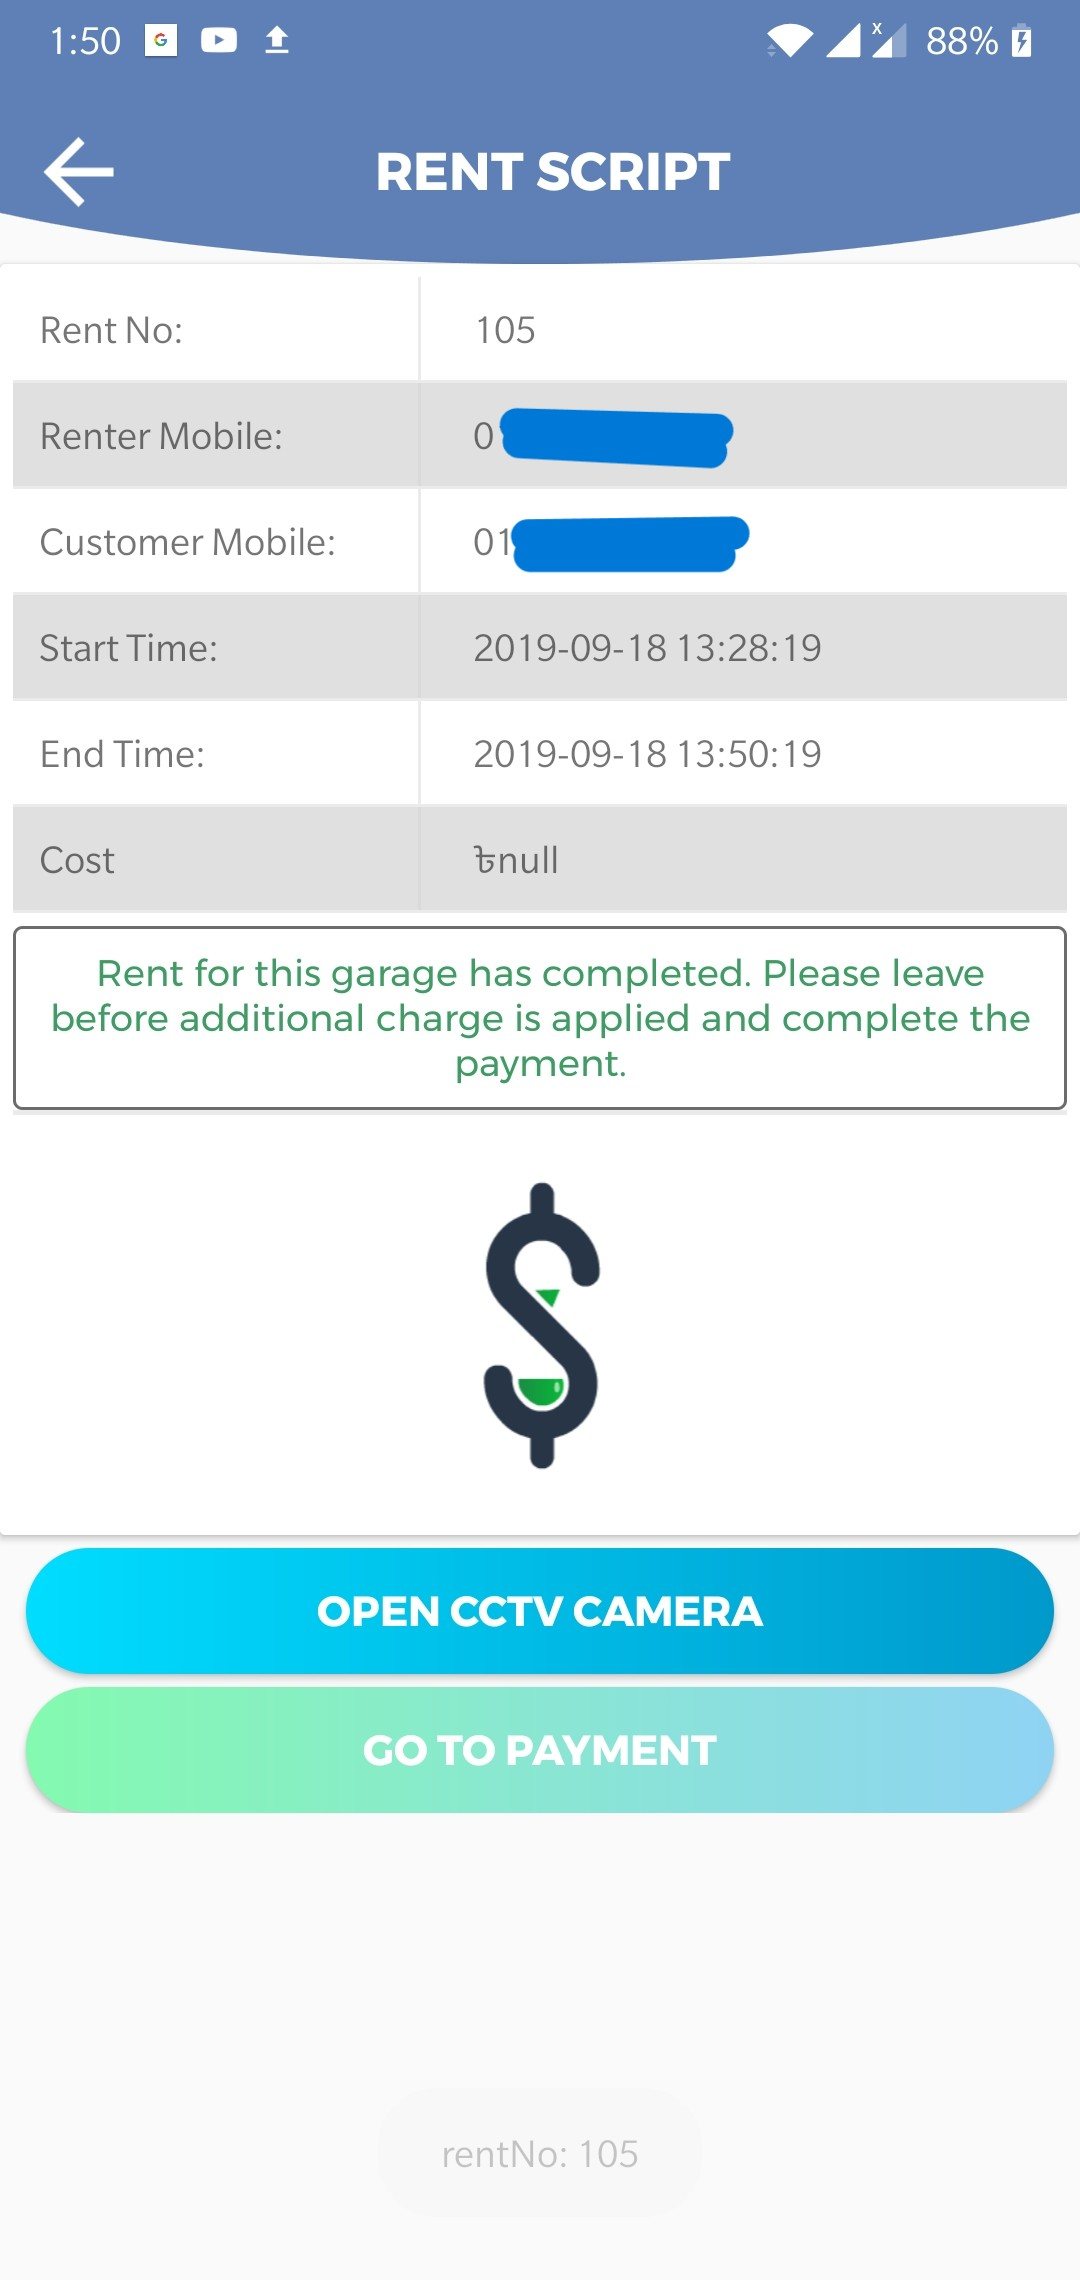
\includegraphics[width=\linewidth]{Payment/payment_notification.jpg}
        \label{arch5}
        \caption{Payment Notifications}
    \end{subfigure}
    \begin{subfigure}[t]{0.4\textwidth}
    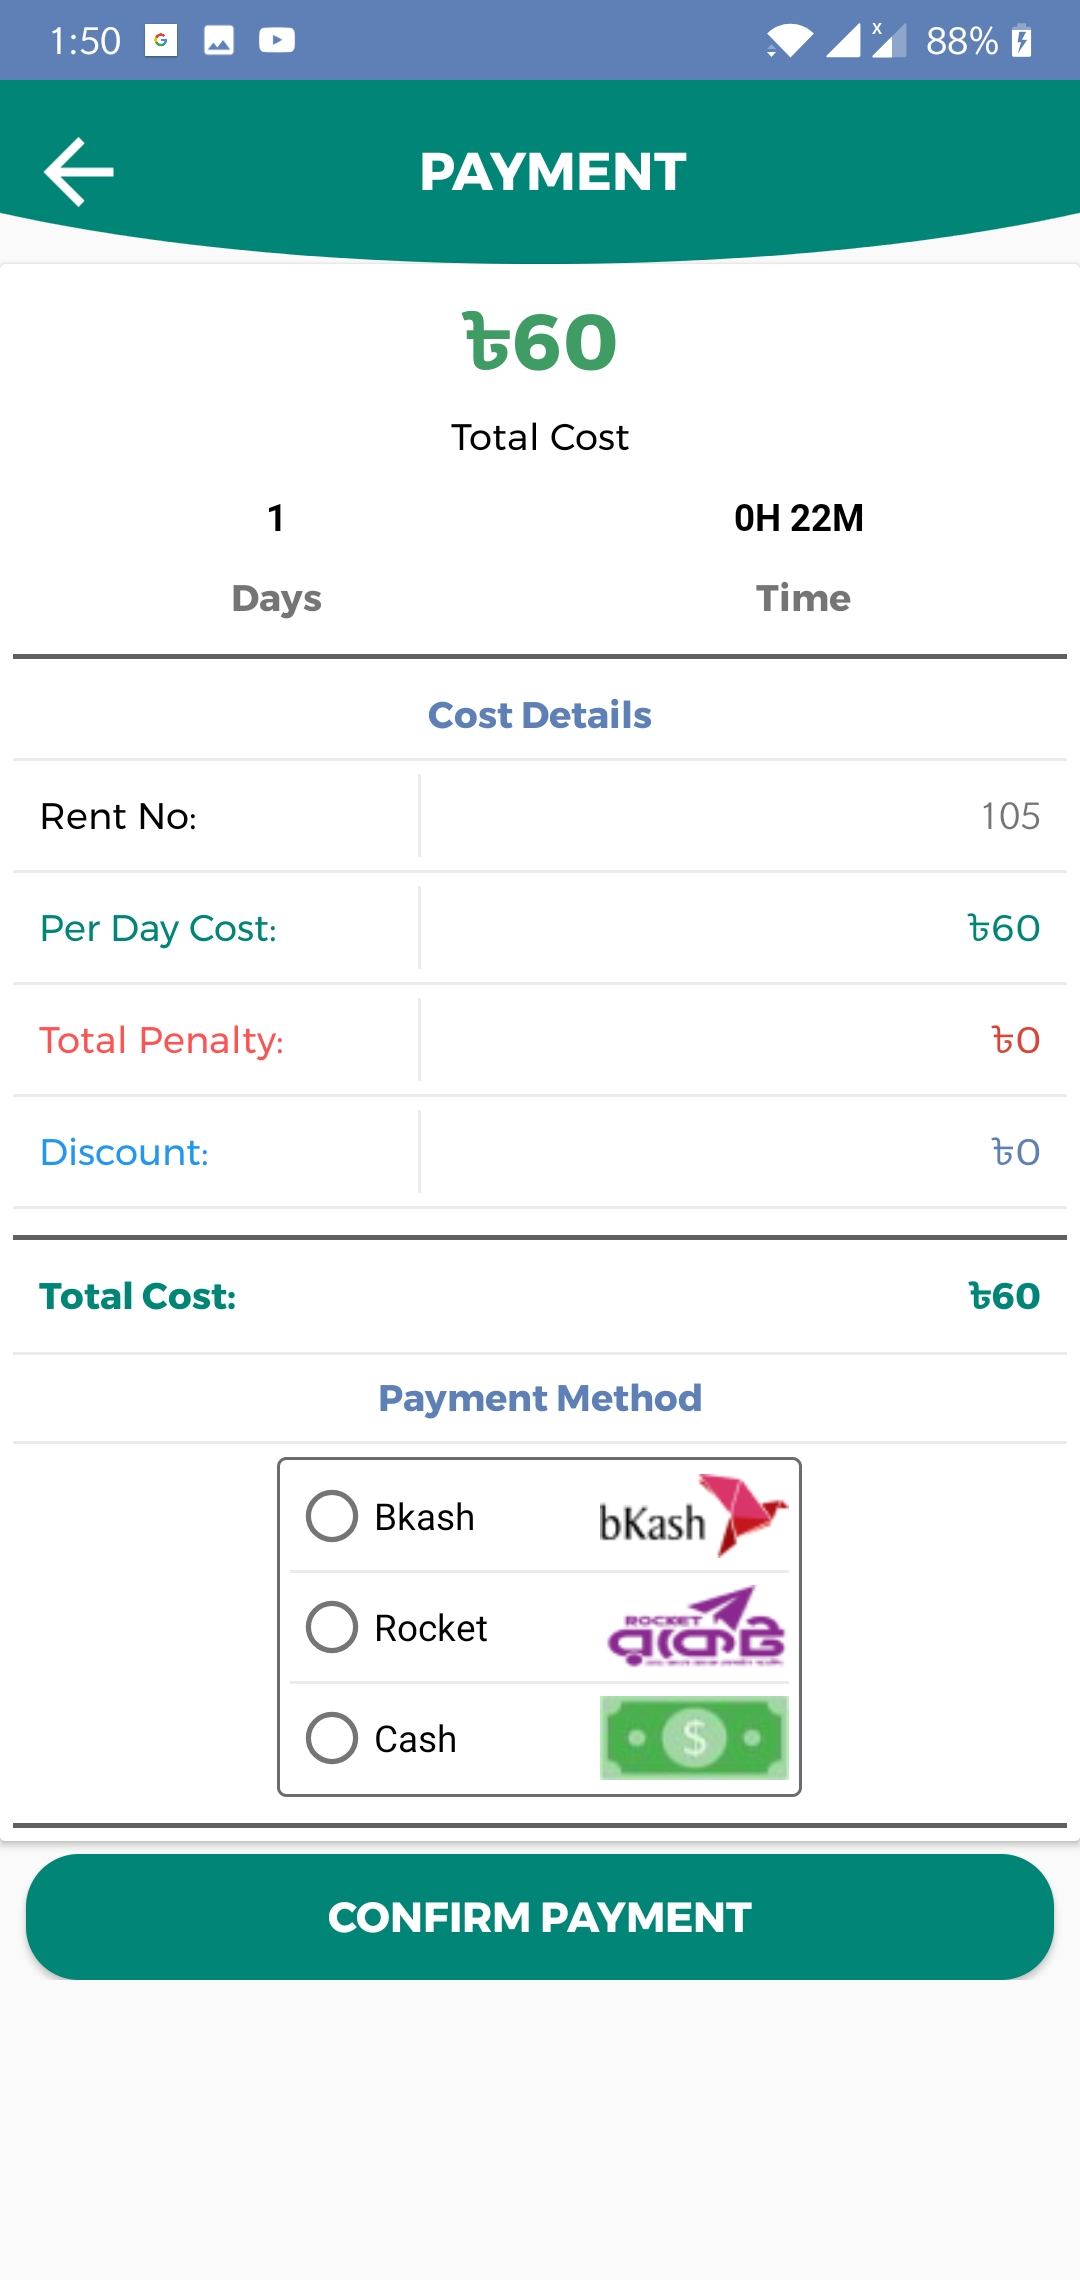
\includegraphics[width=\linewidth]{Payment/payment_window.jpg}
        \label{arch50}
        \caption{Payment Window}
    \end{subfigure}
    \label{fig:arp_os}
\end{figure}
\subsection{Server Side}
%In server side, I am not clear about it.Use necessary snapshots and necessary info.(kotha-barta)
The server side processing will be enabled using PHP and MySQL. The administrator has to control the server side. Whenever a new user registers with the app, the record will be stored in the server side database. When the registered user selects the location and vehicle type, immediately server receives the client’s request. After receiving the request for the desired location, server processes the related information and responds accordingly. Furthermore, the administrator has direct option to view user details and slot details stored on the server direct via the application.There will also be a ongoing server written in java which will run threads to see if rent time is starting for a customer or ending and thus sending proper notifications.
\begin{figure}[h!]
        \begin{minipage}[b]{1\linewidth}
        \centering
        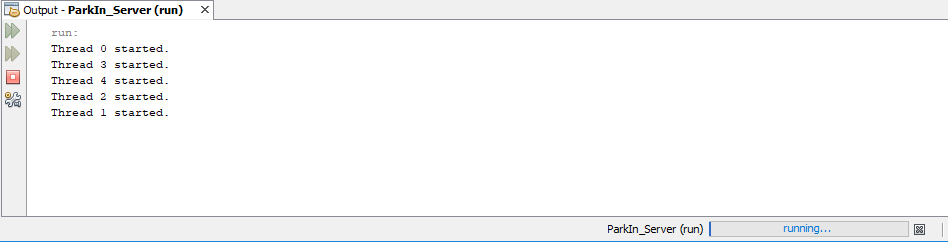
\includegraphics[width=10cm]{parkin_server.png}
        \label{arch40}
        \caption{Server Running}
        \end{minipage}
\end{figure}
\section{Future Scope}
There are some future scope for this project.At this moment,the software does not allow customers to share a space if it is big enough.Although it allows concurrency in different timelines but not during same time.The payment method can be implemented using paid apis like bkash or rocket which is absent from the app at the moment.There is in app communication system between users at the moment which can be added.Also the app doesnot allow extra time allocation at the moment which can be added fairly easily.
\section{Conclusion}
All in all, we think parkin app brings the features which are necessary for a country like us where there is a significant shortage of parking space.Also it allows some users to earn some money through renting their space.We hope that we can continue to make improvement to this project.
\end{document}